\documentclass[10pt]{article}
% Layout of a NeurIPS/ICML submission: single column, 10pt Times, 5.5in x 9in text block.
% Swapping in a venue's style file is a one-line change.
\usepackage[letterpaper,textwidth=5.5in,textheight=9in,top=1in,headsep=0pt,headheight=0pt,footskip=30pt]{geometry}
\usepackage[T1]{fontenc}
\usepackage{times}
\usepackage{microtype}
\usepackage{amsmath,amssymb,amsthm,mathtools}
\usepackage{thm-restate}
\usepackage{booktabs,array}
\usepackage{placeins}
\usepackage{graphicx}
\usepackage[font=small,labelfont=bf]{caption}
\usepackage{tikz}
\usepackage{framed}
\usepackage{needspace}
\usetikzlibrary{positioning,arrows.meta,calc}
\usepackage[round,sort]{natbib}
\renewcommand{\bibfont}{\small\raggedright}
\renewcommand{\bibsection}{\section*{References}\addcontentsline{toc}{section}{References}}
\usepackage[colorlinks,linkcolor=blue!45!black,citecolor=blue!45!black,urlcolor=blue!45!black]{hyperref}
\usepackage[capitalise,noabbrev,nameinlink]{cleveref}
\usepackage{enumitem}
\setlist{nosep,leftmargin=1.4em}
\setlength{\textfloatsep}{10pt plus 2pt minus 2pt}
\renewcommand{\topfraction}{0.85}
\renewcommand{\textfraction}{0.1}

% TeX Live 2026 (LaTeX 2026-06-01) makes a theorem that shares a counter an alias of it (\newcounteralias),
% and thmtools, loaded by thm-restate, would make the same alias again, an error. Leave the alias to LaTeX;
% on older TeX Live, without \newcounteralias, nothing changes.
\makeatletter
\@ifundefined{newcounteralias}{}{%
  \renewcommand\thmt@autorefsetup{\@xa\def\csname\thmt@envname autorefname\@xa\endcsname\@xa{\thmt@thmname}}%
}
\makeatother
\newtheorem{theorem}{Theorem}[section]
\newtheorem{proposition}[theorem]{Proposition}
\newtheorem{corollary}[theorem]{Corollary}
\newtheorem{lemma}[theorem]{Lemma}
\newtheorem{conjecture}{Conjecture}
\theoremstyle{definition}
\newtheorem{definition}[theorem]{Definition}
\newtheorem*{definition*}{Definition}
\theoremstyle{remark}
\newtheorem{remark}[theorem]{Remark}
\crefname{equation}{}{}
\crefname{conjecture}{Conjecture}{Conjectures}
\Crefname{conjecture}{Conjecture}{Conjectures}

\newcommand{\R}{\mathbb{R}}
\newcommand{\Wread}{W_{\mathrm{read}}}
\newcommand{\Wwrite}{W_{\mathrm{write}}}
\newcommand{\dm}{d_{\mathrm{model}}}
\newcommand{\GL}{\mathrm{GL}}
\newcommand{\Ort}{\mathrm{O}}
\newcommand{\CO}{\mathrm{CO}}
\newcommand{\Aff}{\mathrm{Aff}}
% The Frechet derivative, upright to set it apart from the readout D.
\newcommand{\Der}{\mathrm{D}}
\newcommand{\G}{\mathcal{G}}
\newcommand{\norm}[1]{\lVert #1\rVert}
\newcommand{\para}[1]{\smallskip\noindent\textbf{#1}\hspace{0.5em}}
% The one-sentence summary at the start of a main section.
\newcommand{\takeaway}[1]{\noindent\textit{#1}\par\smallskip}
% A link from a result in the main text to its proof in Appendix A.
% A link target at a part of a statement, and references that link name, number and part to it.
\newcommand{\ptlabel}[1]{\phantomsection\label{#1}}
\DeclareRobustCommand{\cpref}[2]{\hyperref[#1:#2]{\cref*{#1}(#2)}}
\DeclareRobustCommand{\Cpref}[2]{\hyperref[#1:#2]{\Cref*{#1}(#2)}}
\DeclareRobustCommand{\rpref}[2]{\hyperref[#1:#2]{\ref*{#1}(#2)}}
\DeclareRobustCommand{\ptlink}[2]{\hyperref[#1:#2]{(#2)}}
\newcommand{\proofin}[1]{\par\vspace{-0.4\baselineskip}\noindent\hfill{\small\itshape Proof in \cref{#1}.}\par\smallskip}
% A main-text result that is a special case of, or follows from, a result in the appendix.
\newcommand{\specialof}[2]{\par\vspace{-0.4\baselineskip}\noindent\hfill{\small\itshape A special case of \cref{#1}, proved in \cref{#2}.}\par\smallskip}
\newcommand{\followsfrom}[2]{\par\vspace{-0.4\baselineskip}\noindent\hfill{\small\itshape Follows from \cref{#1}, proved in \cref{#2}.}\par\smallskip}
% A part of a statement: a link target (if a label is given), a bold number in parentheses and an optional bold name.
\newcommand{\stpart}[3]{\ifx\relax#1\relax\else\ptlabel{#1:#2}\fi{\upshape\bfseries\boldmath(#2)\ifx\relax#3\relax\else\ #3.\fi}}
% A lemma and its proof inside another proof: indented, with a thin gray rule on the left.
\newenvironment{nested}{\par\nopagebreak\def\FrameCommand{\hspace{0.5em}{\color{black!30}\vrule width 0.6pt}\hspace{1em}}\MakeFramed{\advance\hsize-\width\FrameRestore}}{\endMakeFramed}


\title{\Large\bfseries\boldmath Skip Connections Unlock $\dm^2$ Parameters per Layer}

\newif\ifanon \anonfalse
\ifanon
\author{Anonymous authors}
\else
\author{Marko Karbevski$^{*\dagger}$\\ In Simplicity Technologies\\ {\small\texttt{markokarbevski@insimplicity.tech}}\\ {\small\texttt{markokarbevski@gmail.com}}
\and Antonij Mijoski$^{*}$\\ IRMA, Universit\'e de Strasbourg\\ {\small\texttt{antonij.mijoski@unistra.fr}}\\ {\small\texttt{antonijmijo@gmail.com}}}
\fi
\date{}

\begin{document}
\maketitle
\suppressfloats[t]
\ifanon\else
{\renewcommand{\thefootnote}{$*$}%
\footnotetext{\emph{Author contributions.} Marko Karbevski (MK) conceived and led the study, proved the results at depth (\cref{thm:classes,thm:resdepth,thm:exactgain}), and worked on the symmetry breaking across layers and its counting, the parameter counts at model scale, the experiments and the applications. Antonij Mijoski (AM) worked on the writing. All of MK's work on the results, the proofs and the experiments was done with AI assistants.}}
{\renewcommand{\thefootnote}{$\dagger$}\footnotetext{Corresponding author.}}
\fi
\vspace{-1.5em}

\begin{abstract}
Residual and skipless networks with the same blocks have the same parameters. Do they use them alike? Here we show that skip connections unlock $\dm^2$ parameters per block, or $\dm(\dm-1)/2$ under RMSNorm, where $\dm$ is the hidden dimension. Without skips, every hidden state has a free basis: the next block undoes any change of basis. A skip adds the old hidden state to the new one, tying these bases into one. Fixing each free basis removes exactly that many parameters, $8.5$ percent of a skipless LayerNorm ViT-B. Where symmetries are the only redundancy, the skips raise the functional dimension, the number of directions in which parameters move the function, by as much. For continuous inputs, we prove the exact gain without normalization for one block and for $\tanh$ networks; with or without RMSNorm, at least this gain at any depth for attention, $\tanh$, GELU, SwiGLU and GeGLU networks.
\end{abstract}

\section{Introduction}\label{sec:intro}

Skip connections are a building block of almost every deep network trained today \citep{he2016resnet}. The usual reason is training: skips make deep networks easier to optimize \citep{he2016resnet,balduzzi2017shattered,orhan2018skip}. Recent skipless models challenge the need for skips. \citet{ji2026cutting} remove every skip from a ViT-B \citep{dosovitskiy2021an} and train it on ImageNet-1k, where it outperforms the residual ViT-B in top-1 accuracy, and \citet{he2023shortcuts,he2024simplifying} train transformers without skips.

So what do skips change, besides training? A residual network adds the input of every block to its output through an \emph{identity skip}, and a skipless network returns the output alone. The two have the same parameters. We ask whether they use them alike. Throughout, a network starts with a linear embedding and ends with a linear readout, the unembedding, and its hidden states, in between, have dimension $\dm$. In a pre-RMSNorm network, every block and the readout read their input through RMSNorm, which divides each token by its root mean square, regularized by a constant $\varepsilon > 0$.

\para{Hidden states have units.} Think of the coordinates of a hidden state as units of measurement, such as meters or feet. Without normalization, every hidden state of a skipless network can change its units. Let $G$ be an invertible $\dm\times\dm$ matrix, and let hidden states be row vectors $h$. If the matrix $W$ that writes the output of a block becomes $WG$, and the matrix $W'$ through which the next block reads it becomes $G^{-1}W'$, the next block sees $hG\,G^{-1}W' = hW'$, and the function does not change. A skip adds the old hidden state to the new one, and only quantities in the same units can be added. So the skips tie the units of all hidden states into one.

\para{Free bases are removable parameters.} Each such $G$ can be spent to set a $\dm\times\dm$ submatrix of the weights to the identity, which removes $\dm^2$ parameters without changing the function. A skipless network of $L$ blocks has $L+1$ hidden states, so $(L+1)\dm^2$ of its parameters are removable; a residual network keeps one free change of basis, so $\dm^2$. Under RMSNorm only orthogonal matrices pass through the normalization, and a QR factorization makes the submatrix triangular instead, which removes the $\dm(\dm-1)/2$ entries below its diagonal at each hidden state. With LayerNorm, which acts as RMSNorm in dimension $\dm - 1$, the skipless ViT-B loses $8.5$ percent of its parameters this way (\cref{sec:trained}).

\para{Fewer parameters, the same functions.} For almost every choice of weights, removing these parameters does not change the function. What the skips change is the functional dimension, the number of independent directions in which the parameters move the function \citep{grigsby2022functional}. Our running example, without biases or normalization, has an embedding $\R^6 \to \R^4$, so $\dm = 4$, then $L = 3$ MLP blocks with $8$ hidden GELU units each, and a readout $\R^4 \to \R^6$: $P = 240$ parameters. Of these, $64$ are removable without skips and $16$ with them. The functional dimension is $176$ without skips and $224$ with them (\cref{fig:gelu}): the skips unlock $L\dm^2 = 48$ parameters.

\para{Known symmetries.} Permuting the hidden units or heads of a block, and flipping the signs of $\tanh$ units, preserve the function \citep{sussmann1992,fefferman1994,theus2025glmc}; these symmetries are finite and remove no parameters. Rescaling a ReLU unit preserves the function too \citep{rolnick2020reverse,godfrey2022symmetries} and removes one parameter, so a block of $4\dm$ units loses $4\dm$ parameters to rescalings, against $\dm^2$ to a change of basis. Rescalings and the changes of basis inside attention heads \citep{wang2025gauge,theus2025glmc} act inside a block, alike with and without skips, so they cancel when the two networks are compared. Changes of basis at hidden states are known too \citep{zhao2023symmetries}, and so is one rotation of the residual stream under RMSNorm \citep{ashkboos2024slicegpt,theus2025glmc}, the one change of basis that the skips leave. In residual ReLU networks, permutations and rescalings of the hidden states preserve the function when they agree at all hidden states that the skips join \citep[Remark~3.6]{godfrey2022symmetries}. Beyond these, we count the $L\dm^2$ dimensions of symmetry that the skips remove, and show when they become functional dimension.

\begin{figure}[t]
\centering
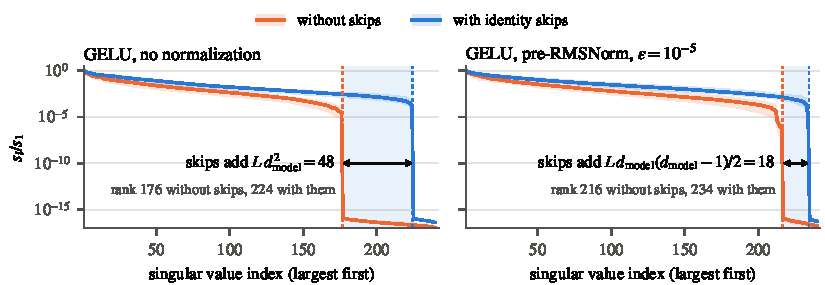
\includegraphics[width=0.94\linewidth]{figs/spectra_gelu.pdf}
\caption{Singular values of the Jacobian of the parameter-to-output map on $4000$ Gaussian inputs, with and without skips at the same weights, for the running example; median and range over $20$ weight draws. Skips raise its rank, the functional dimension, by $48$, and by $18$ under RMSNorm.}
\label{fig:gelu}
\end{figure}

\para{Contributions.}
\begin{enumerate}[label=\arabic*.]
\item \emph{Exact reduction} (\cref{sec:skipless}). The change of basis at each hidden state of a skipless network sets one $\dm\times\dm$ submatrix of its weights to the identity. \citet{zhao2023symmetries} describe this symmetry, and \citet{graef2024tricks} uses an instance of it to remove weights from skipless transformers; here it is a general tool.
\item \emph{Learned skips are identity units} (\cref{sec:learned}). A learned skip adds $hA$ in place of $h$, for a trainable $\dm\times\dm$ matrix $A$. It is a block of $\dm$ hidden units whose activation is the identity. The same tool turns $A$ into the identity: without normalization, a network with invertible learned skips is a residual network. Under RMSNorm, learned skips become triangular.
\item \emph{One change of basis is left} (\cref{sec:global}). A residual network keeps one change of basis for all its hidden states. When the embedding and the readout count among the parameters, this change of basis is a counterexample to the statement of \citet{wang2025gauge} that the symmetry group of a transformer is the product of the groups of its blocks.
\item \emph{Skips unlock functional dimension} (\cref{sec:gain}). Where the symmetries are the only redundancy, the skips raise the functional dimension by $\dm^2$ per block, and by $\dm(\dm-1)/2$ under RMSNorm. Inputs are continuous, which excludes one-hot tokens. Without normalization we prove this gain for one block, attention included, and for networks of $\tanh$ blocks or of GELU blocks with at least $2\dm$ hidden units. At any depth, with or without pre-RMSNorm, we prove at least this gain for attention, $\tanh$, GELU, SwiGLU and GeGLU blocks. Hence almost no such residual network equals a skipless network of the same widths. We measure the gain in deeper MLPs and small transformers.
\end{enumerate}
\Cref{tab:results} lists the results. \Cref{sec:setup} fixes the setting, \cref{sec:reduce} removes parameters and \cref{sec:gain} counts functional dimension; proofs are in the appendix.

\begin{table}[t]
\centering\small
\renewcommand{\arraystretch}{1.1}
\newcommand{\rtag}[3]{\if\relax\detokenize{#3}\relax\hyperref[#2]{#1~\ref*{#2}}\else\hyperref[#2:#3]{#1~\ref*{#2}(#3)}\fi}
\begin{tabular}{@{}llll@{}}
\toprule
\textbf{Proven} & \textbf{Value} & \textbf{Blocks} & \textbf{Result} \\
\midrule
\multicolumn{4}{@{}l}{\emph{Parameters removed exactly, without changing the function}} \\
\quad without skips & $(L+1)\dm^2$ & all & \rtag{Prop.}{prop:skipless}{} \\
\quad\quad with pre-RMSNorm & $(L+1)\dm(\dm-1)/2$ & all & \rtag{Thm.}{thm:rmstri}{i} \\
\quad learned skips & $L\dm^2$, every skip entry & all & \rtag{Thm.}{thm:learned}{} \\
\quad\quad with pre-RMSNorm & $L\dm(\dm-1)/2$ & all & \rtag{Thm.}{thm:rmstri}{iv} \\
\quad identity skips & $\dm^2$ & all & \rtag{Thm.}{thm:tie}{iii} \\
\quad\quad with pre-RMSNorm & $\dm(\dm-1)/2$ & all & \rtag{Thm.}{thm:rmstri}{iii} \\
\midrule
\multicolumn{4}{@{}l}{\emph{Dimensions of symmetry removed by the skips}} \\
\quad any $L$ & $L\dm^2$ & all & \rtag{Thm.}{thm:tie}{ii} \\
\quad\quad with pre-RMSNorm & $L\dm(\dm-1)/2$ & all & \rtag{Thm.}{thm:rmstri}{ii} \\
\midrule
\multicolumn{4}{@{}l}{\emph{Functional dimension added by the skips}} \\
\quad $L = 1$ & exactly $\dm^2$ & all & \rtag{Thm.}{thm:oneblock}{i} \\
\quad\quad with pre-RMSNorm & at least $\dm(\dm-1)/2$ & all & \rtag{Thm.}{thm:oneblock}{ii} \\
\quad $L \ge 2$ & at least $L\dm^2$ & smooth & \rtag{Thm.}{thm:resdepth}{} \\
\quad\quad with pre-RMSNorm & at least $L\dm(\dm-1)/2$ & smooth & \rtag{Thm.}{thm:resdepth}{} \\
\quad $L \ge 2$ & exactly $L\dm^2$ & $\tanh$ & \rtag{Thm.}{thm:exactgain}{i} \\
\quad $L \ge 2$ & exactly $L\dm^2$ & GELU, $\ge 2\dm$ units & \rtag{Thm.}{thm:exactgain}{ii} \\
\midrule
\multicolumn{4}{@{}l}{\emph{Residual networks that equal a skipless network}} \\
\quad same widths, any $L$ & measure zero & smooth & \rtag{Thm.}{thm:classes}{i} \\
\quad\quad with pre-RMSNorm & measure zero & smooth & \rtag{Thm.}{thm:classes}{i} \\
\quad $< L\dm/2$ more units & measure zero & GELU & \rtag{Thm.}{thm:classes}{ii} \\
\bottomrule
\end{tabular}
\caption{The results, for networks of $L$ blocks with hidden states of dimension $\dm$, at generic parameters; scope in \cref{sec:setup}. All: every block of \cref{sec:setup}. Smooth: attention, $\tanh$, GELU, SwiGLU and GeGLU blocks. Measured at depth: \cref{tab:measured}.}
\label{tab:results}
\end{table}

\section{Setup}\label{sec:setup}
\takeaway{A block reads a hidden state, applies a fixed map and writes back; a network chains blocks between an embedding and a readout, with or without skips.}

\para{Blocks.} A hidden state is a matrix $h \in \R^{T\times\dm}$ whose rows are the $T$ tokens of a sequence. A block reads it with a trainable matrix $\Wread$, the \emph{read}, applies a fixed map $f$, and writes the result with a trainable matrix $\Wwrite$, the \emph{write}:
\begin{equation}\label{eq:block}
B(h) = f(h\Wread)\,\Wwrite.
\end{equation}
We keep the word block for these maps, and say submatrix for a block of a matrix. In an MLP block with $m$ hidden units, its width, $\Wread \in \R^{\dm\times m}$, $\Wwrite \in \R^{m\times\dm}$, and $f$ applies an activation to every unit of every token: $\tanh$, GELU, ReLU, or its square, ReLU$^2$. In a gated block the read has $2m$ columns, which give each token a gate $g_i$ and a value $v_i$ for each unit, and $f$ maps them to $\sigma(g_i)\,v_i$, with $\sigma$ the ReLU in ReGLU, SiLU in SwiGLU and GELU in GeGLU \citep{shazeer2020glu}. In an attention block with $H$ heads of width $d_h$, the read holds the query, key and value matrices $W_Q$, $W_K$ and $W_V$ of all heads, $f$ is the attention map, and the write is the output projection $W_O$; the width of the block is $Hd_h$.

\para{Networks.} A network maps an input $x \in \R^{T\times d_{\mathrm{in}}}$ to
\begin{equation}\label{eq:nets}
\mathcal M(x) = C \circ D \circ (A_L + B_L) \circ \dots \circ (A_1 + B_1) \circ E\,(x),
\end{equation}
where $E$ is the linear embedding $x \mapsto xE$, with $E \in \R^{d_{\mathrm{in}}\times\dm}$, $B_\ell$ is block $\ell$, $D$ is the linear readout, or unembedding, $h \mapsto hD$, with $D \in \R^{\dm\times d_{\mathrm{out}}}$, and $A_\ell$ is the skip of block $\ell$, the map $h \mapsto hA_\ell$: $A_\ell = 0$ in a \emph{skipless} network, $A_\ell = I$ in a \emph{residual} network, and a trainable $\dm\times\dm$ matrix in a network with \emph{learned skips}. So $h_0 = xE$, $h_\ell = h_{\ell-1}A_\ell + B_\ell(h_{\ell-1})$ and $y = h_LD$. The output function $C$ is set by the task, for example the identity for regression and the softmax for multiclass classification \citep[Sections~5.1 and~5.2]{bishop2006pattern}. It has no weights, and we ignore it: functions, equality and functional dimension below are those of the map $x \mapsto y$. The skipless and the residual network have the same $P$ parameters. A transformer layer has two blocks, its attention and MLP sub-layers, so $L$ counts sub-layers, and \emph{per block} means per layer of an MLP and per sub-layer of a transformer.

\para{Normalization.} In a \emph{pre-RMSNorm} network the blocks and the readout read $N(h)$ in place of $h$, where $N$ divides each row $v$ of $h$ by $\sqrt{\norm{v}^2/\dm + \varepsilon}$, with $\varepsilon > 0$. Skips read $h$ itself, so a residual network computes $h_\ell = h_{\ell-1} + B_\ell\big(N(h_{\ell-1})\big)$ and $y = N(h_L)D$. A learned gain after $N$ is folded into the next read.

\para{Scope.} For simplicity, networks have no biases. Every MLP block has at least $\dm$ hidden units, and all MLP blocks of a network are of one kind. All attention blocks have the same number of heads, of width at most $\dm$ and of total width $Hd_h \ge \dm$, and act on sequences of at least two tokens. Inputs are continuous: they range over all of $\R^{T\times d_{\mathrm{in}}}$, which excludes one-hot tokens, and $d_{\mathrm{in}}, d_{\mathrm{out}} \ge \dm \ge 2$. The exact reductions of \cref{sec:reduce} hold for any inputs, and with biases. Most results hold more generally, and the appendix states them so. A statement holds at \emph{generic} parameters if it holds outside a set of Lebesgue measure zero. Attention, $\tanh$, GELU, SwiGLU and GeGLU blocks are \emph{smooth}; for them, any open set of inputs gives the same results.

\section{Free changes of basis remove parameters exactly}\label{sec:reduce}\label{sec:gauge}
\takeaway{Without normalization, every change of basis that a network keeps can set a $\dm\times\dm$ submatrix of its weights to the identity without changing its function: one per hidden state without skips, and one in all with identity skips. A learned skip is itself such a submatrix, and becomes the identity. Under RMSNorm, these submatrices become triangular.}

\subsection{Without skips: one free submatrix per hidden state}\label{sec:skipless}\label{sec:junctions}

Without normalization, nothing nonlinear happens between the write of one block and the read of the next, so the basis of the hidden state between them is free. For an invertible $\dm\times\dm$ matrix $G$, the \emph{change of basis} $G$ at $h_\ell$ maps
\begin{equation}\label{eq:cob}
W \mapsto WG \ \text{ for the writes into } h_\ell, \qquad W \mapsto G^{-1}W \ \text{ for the reads of } h_\ell.
\end{equation}
The writes into $h_\ell$ are $\Wwrite^{\ell}$, or $E$ if $\ell = 0$, and the reads of $h_\ell$ are $\Wread^{\ell+1}$, or $D$ if $\ell = L$. The hidden state becomes $h_\ell G$, and each read computes $h_\ell G\,G^{-1}W = h_\ell W$ as before, so the function does not change (\cref{fig:junctions}b).

A symmetry can be spent.

\begin{restatable}[One free submatrix per hidden state]{proposition}{propSkipless}\label{prop:skipless}
Without normalization, let $\dm$ columns of the read of $h_\ell$ in a skipless network form an invertible matrix $W_1$. The change of basis $G = W_1$ at $h_\ell$ preserves the function and turns $W_1$ into the identity. At generic parameters every hidden state has such columns, and these changes of basis at all $L+1$ hidden states remove $(L+1)\dm^2$ parameters.
\end{restatable}
\specialof{prop:normalform}{app:prf-normalform}

Rows of a write work too: if $\dm$ rows of the write into $h_\ell$ form an invertible matrix, the change of basis by its inverse turns them into the identity. In a skipless transformer with $Hd_h = \dm$, $G = W_Q$ before an attention block sets its queries to the identity, and $G = W_O^{-1}$ after it sets its output projection to the identity: $2\dm^2$ parameters per layer. This is how \citet{graef2024tricks} removes $15$ percent of the weights of a skipless Mistral-7B.

So skipless networks with one identity submatrix per hidden state compute, up to a set of weights of measure zero, the same functions with $(L+1)\dm^2$ fewer parameters. \Cref{sec:gain} asks what this means for the size of a network.

\begin{figure}[t]
\centering
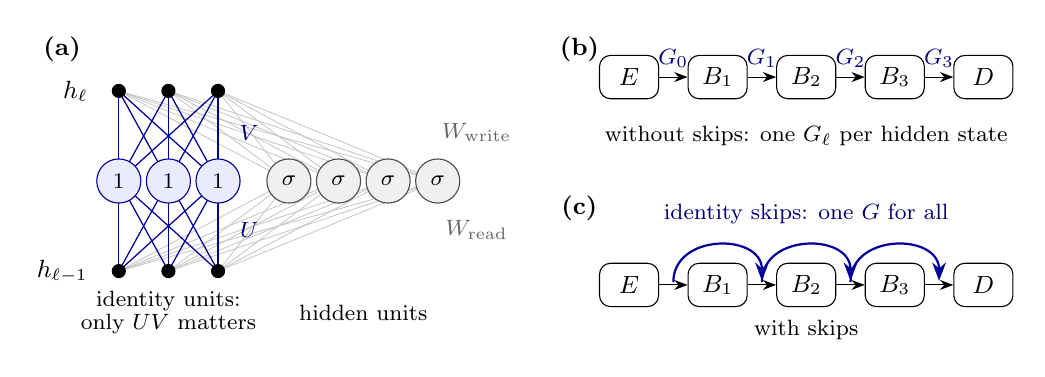
\begin{tikzpicture}[x=0.9mm,y=0.88mm,>=Stealth,
  blk/.style={draw,rounded corners,minimum width=7.5mm,minimum height=5.5mm,font=\small},
  lab/.style={font=\footnotesize,text=blue!45!black},
  panel/.style={font=\small\bfseries},
  io/.style={circle,fill=black,inner sep=0pt,minimum size=1.8mm},
  lin/.style={circle,draw=blue!60!black,fill=blue!8,minimum size=5.6mm,inner sep=0pt,font=\footnotesize},
  sig/.style={circle,draw=black!70,fill=gray!12,minimum size=5.6mm,inner sep=0pt,font=\footnotesize},
  idedge/.style={blue!60!black,line width=0.45pt},
  branchedge/.style={gray!45,line width=0.3pt}]
% (a) a block with a learned skip, as one wide block
\node[panel] at (-4,40) {(a)};
\foreach \i/\x in {1/4,2/11,3/18} {
  \coordinate (in\i)  at (\x,8);
  \coordinate (lin\i) at (\x,21);
  \coordinate (out\i) at (\x,34);
}
\foreach \k/\x in {1/28,2/35,3/42,4/49} \coordinate (sg\k) at (\x,21);
\foreach \i in {1,2,3} \foreach \k in {1,...,4} {\draw[branchedge] (in\i)--(sg\k); \draw[branchedge] (sg\k)--(out\i);}
\foreach \i in {1,2,3} \foreach \j in {1,2,3} {\draw[idedge] (in\i)--(lin\j); \draw[idedge] (lin\j)--(out\i);}
\foreach \i in {1,2,3} {\node[io] at (in\i) {}; \node[io] at (out\i) {}; \node[lin] at (lin\i) {$1$};}
\foreach \k in {1,...,4} \node[sig] at (sg\k) {$\sigma$};
\node[anchor=east,font=\small] at (1,8)  {$h_{\ell-1}$};
\node[anchor=east,font=\small] at (1,34) {$h_{\ell}$};
\node[lab] at (22.4,14) {$U$};
\node[lab] at (22.4,28) {$V$};
\node[font=\footnotesize,text=black!60] at (54.5,14) {$\Wread$};
\node[font=\footnotesize,text=black!60] at (54.5,28) {$\Wwrite$};
\node[align=center,font=\footnotesize] at (11,2) {identity units:\\[-1pt] only $UV$ matters};
\node[align=center,font=\footnotesize] at (38.5,2) {hidden units};
% (b) a skipless network: a free change of basis at every hidden state
\def\ox{76}
\node[panel] at ({\ox-7},40) {(b)};
\node[blk] (a0) at (\ox,36) {$E$};
\node[blk] (a1) at ({\ox+12.5},36) {$B_1$};
\node[blk] (a2) at ({\ox+25},36) {$B_2$};
\node[blk] (a3) at ({\ox+37.5},36) {$B_3$};
\node[blk] (a4) at ({\ox+50},36) {$D$};
\foreach \i/\j in {0/1,1/2,2/3,3/4} \draw[->] (a\i)--(a\j) node[midway,above,lab]{$G_{\i}$};
\node[font=\footnotesize] at ({\ox+25},27.5) {without skips: one $G_\ell$ per hidden state};
% (c) the residual network: one change of basis for all hidden states
\node[panel] at ({\ox-7},17) {(c)};
\node[blk] (b0) at (\ox,6) {$E$};
\node[blk] (b1) at ({\ox+12.5},6) {$B_1$};
\node[blk] (b2) at ({\ox+25},6) {$B_2$};
\node[blk] (b3) at ({\ox+37.5},6) {$B_3$};
\node[blk] (b4) at ({\ox+50},6) {$D$};
\foreach \i/\j in {0/1,1/2,2/3,3/4} \draw[->] (b\i)--(b\j);
\foreach \x in {12.5,25,37.5} \draw[->,thick,blue!60!black] ({\ox+\x-6.25},6.4) .. controls ({\ox+\x-6.25},13.5) and ({\ox+\x+6.25},13.5) .. ({\ox+\x+6.25},6.6);
\node[lab] at ({\ox+25},16.3) {identity skips: one $G$ for all};
\node[font=\footnotesize] at ({\ox+25},-0.5) {with skips};
\end{tikzpicture}
\caption{(a)~A block with a learned skip is a block with $\dm$ identity units, read by $U$ and written by $V$. (b)~Without skips, every hidden state has its own change of basis $G_\ell$. (c)~Identity skips carry each hidden state into the next, so one change of basis is left.}
\label{fig:junctions}
\end{figure}

\subsection{Learned skips are blocks of identity units}\label{sec:learned}

A learned skip, which adds $hA$ in place of $h$, is a block in disguise: $\dm$ hidden units whose activation is the identity \citep[Section~4]{lin2018resnet}. Read them with a matrix $U$ and write them with a matrix $V$, so that $A = UV$. The block with this skip is then a wider block of the form \eqref{eq:block} (\cref{fig:junctions}a):
\begin{equation}\label{eq:mixed}
h\,UV + f(h\Wread)\,\Wwrite \;=\; \tilde f\big(h\,[\,U \mid \Wread\,]\big)\begin{bmatrix} V \\ \Wwrite \end{bmatrix}, \qquad \tilde f\big([\,u \mid z\,]\big) = \big[\,u \mid f(z)\,\big].
\end{equation}
The tool of \cref{sec:skipless} now applies twice.

\para{Merge.} Nothing nonlinear happens between $U$ and $V$, so the identity units have their own change of basis, $(U, V) \mapsto (UK, K^{-1}V)$, and only $A = UV$ enters the function. When $A$ is invertible, $K = V$ gives the read $UV = A$ and the write $I$: one matrix, the skip.

\para{Reduce.} The skip $A_\ell$ reads $h_{\ell-1}$ and writes $h_\ell$, so changes of basis at the two hidden states map it to $G_{\ell-1}^{-1}A_\ell G_\ell$. As a $\dm\times\dm$ submatrix of a read of $h_{\ell-1}$, it becomes the identity under $G_{\ell-1} = A_\ell$, as in \cref{prop:skipless}. This multiplies the skip before it, $A_{\ell-1}$, by $A_\ell$. Sweeping from the readout back turns every skip into the identity, and the product of all skips ends up in the embedding. Let $\Lambda_\ell = A_{\ell+1}\cdots A_L$, with $\Lambda_L = I$.

\begin{restatable}[Learned skips are identity skips]{theorem}{thmLearned}\label{thm:learned}
Without normalization, let every learned skip $A_\ell$ be invertible. The network with learned skips computes the same function as the residual network with the embedding $E\Lambda_0$, the reads $\Lambda_{\ell-1}^{-1}\Wread^{\ell}$, the writes $\Wwrite^{\ell}\Lambda_\ell$ and the readout $D$.
\end{restatable}
\specialof{thm:gaugefull}{app:prf-gauge}

So all $L\dm^2$ parameters of the learned skips can go: without normalization, invertible learned skips compute the same functions as identity skips, and \cref{sec:count} shows that they have the same functional dimension.

\subsection{Identity skips tie the hidden states}\label{sec:global}\label{sec:gaugefix}

After the sweep one change of basis is left, and it must be the same at all hidden states. With a change of basis $G_{\ell-1}$ at $h_{\ell-1}$ and $G_\ell$ at $h_\ell$, a residual block computes
\begin{equation}\label{eq:defect}
h_{\ell-1}G_{\ell-1} + B_\ell(h_{\ell-1})\,G_\ell \;=\; h_\ell G_\ell + h_{\ell-1}(G_{\ell-1} - G_\ell).
\end{equation}
The skip carries $h_{\ell-1}$ in the basis $G_{\ell-1}$, and the block writes in the basis $G_\ell$, like feet added to meters. Unless the two agree, the defect $h_{\ell-1}(G_{\ell-1} - G_\ell)$ reaches every later block.

\begin{restatable}[One change of basis is left]{theorem}{thmTie}\label{thm:tie}
Without normalization, let $G_0, \dots, G_L$ be invertible.\\
\stpart{thm:tie}{i}{} The map $E \mapsto EG_0$, $\Wread^{\ell} \mapsto G_{\ell-1}^{-1}\Wread^{\ell}$, $\Wwrite^{\ell} \mapsto \Wwrite^{\ell}G_\ell$, $D \mapsto G_L^{-1}D$ preserves the function of every residual network if and only if $G_0 = G_1 = \dots = G_L$.\\
\stpart{thm:tie}{ii}{} The changes of basis that preserve the function at all parameters form a group of dimension $(L+1)\dm^2$ in a skipless network and $\dm^2$ in a residual one.\\
\stpart{thm:tie}{iii}{} In a residual network, let $\dm$ columns of any one read form an invertible matrix $W_1$. The same change of basis $W_1$ at all hidden states preserves the function and turns $W_1$ into the identity.
\end{restatable}
\proofin{app:prf-gauge}

So the $L$ skips remove $L\dm^2$ dimensions of symmetry. In the language of gauge theory, they turn a symmetry that is local in depth into a global one \citep{hashimoto2024unification}. Where a block outweighs its skip, the defect is small, and separate changes of basis on its two sides are approximate symmetries \citep[Section~6.4]{gong2026aro}.

\para{A counterexample.} \citet[Theorem~7]{wang2025gauge} state that the symmetry group of a transformer is the product of the groups of its blocks. When the embedding and the readout count among the parameters, the change of basis that the skips leave is a counterexample: it changes the embedding, which no element of that product does. Two instances of it preserve the function of common transformers. A global permutation of the coordinates of the hidden states does for every placement of the normalization, as \citet[Section~3.3]{verma2024merging} use to merge BERT models. A global rotation does in pre-RMSNorm models with an untied readout, the construction behind Theorem~1 of \citet{ashkboos2024slicegpt} (\cref{app:product}).

\subsection{Under RMSNorm: orthogonal maps pass, triangles stay}\label{sec:norm}

With pre-RMSNorm, the network with learned skips computes
\begin{equation}\label{eq:prenorm}
h_\ell = h_{\ell-1}A_\ell + B_\ell\big(N(h_{\ell-1})\big), \qquad y = N(h_L)\,D.
\end{equation}
A change of basis $G$ at $h_\ell$ now reaches the reads through $N$, as $N(h_\ell G)$. Orthogonal matrices pass: $N(hQ) = N(h)Q$ for every orthogonal $Q$, since $N$ only rescales each row, and the read absorbs $Q$ by $W \mapsto Q^\top W$. Since $\varepsilon > 0$, no other invertible matrix passes (\cref{lem:rms}). So every hidden state of a skipless network, or of one with learned skips, keeps an orthogonal change of basis, $\dm(\dm-1)/2$ dimensions. It cannot turn a submatrix into the identity, but a QR factorization shows that it can make it triangular.

\begin{restatable}[Triangles under RMSNorm]{theorem}{thmRMSTri}\label{thm:rmstri}
Consider pre-RMSNorm networks.\\
\stpart{thm:rmstri}{i}{} In a skipless network, let $\dm$ columns of the read of $h_\ell$ form a matrix $W_1 = QR$, with $Q$ orthogonal and $R$ upper triangular. The change of basis $Q$ at $h_\ell$ preserves the function and turns $W_1$ into $R$; at all $L+1$ hidden states, these changes of basis remove $(L+1)\dm(\dm-1)/2$ parameters.\\
\stpart{thm:rmstri}{ii}{} The changes of basis that preserve the function at all parameters are orthogonal, and in a residual network they agree at all hidden states. They form a group of dimension $(L+1)\dm(\dm-1)/2$ in a skipless network and $\dm(\dm-1)/2$ in a residual one.\\
\stpart{thm:rmstri}{iii}{} In a residual network, let $\dm$ columns of any one read form a matrix $W_1 = QR$. The same change of basis $Q$ at all hidden states preserves the function and turns $W_1$ into $R$.\\
\stpart{thm:rmstri}{iv}{Triangular skips} If every learned skip $A_\ell$ is invertible, there are orthogonal $Q_1, \dots, Q_L$, with $Q_0 = I$, such that every $Q_{\ell-1}^\top A_\ell Q_\ell$ is upper triangular, and the network with these skips, the reads $Q_{\ell-1}^\top\Wread^{\ell}$, the writes $\Wwrite^{\ell}Q_\ell$ and the readout $Q_L^\top D$ computes the same function.
\end{restatable}
\proofin{app:prf-rms}

\para{What a learned skip carries.} Write a skip as an upper triangular matrix times an orthogonal one. The orthogonal factor, of dimension $\dm(\dm-1)/2$, is removable: \cpref{thm:rmstri}{iv} spends the changes of basis on it. The $\dm(\dm+1)/2$ entries of the triangular factor stay, and an identity skip fixes them as well. So under RMSNorm an identity skip does two things: it ties the change of basis at $h_\ell$ to the one at $h_{\ell-1}$, and it fixes the triangle, a constraint that \cref{sec:count} counts.

LayerNorm is RMSNorm after a projection that removes the mean of each row, and it reduces to RMSNorm of dimension $\dm - 1$ (\cref{prop:ln}). Every RMSNorm count above then holds with $\dm - 1$ in place of $\dm$: $(\dm-1)(\dm-2)/2$ per hidden state.

\subsection{What trained models give up}\label{sec:trained}

\para{A skipless ViT-B.} The skipless ViT-B of \citet{ji2026cutting} has $\dm = 768$ and $25$ hidden states: one before each of its $24$ blocks and one before the readout. With standard pre-LayerNorm blocks, which reduce to RMSNorm of dimension $767$, each hidden state keeps an orthogonal change of basis. One triangular $767\times767$ submatrix of a read per hidden state removes $25\cdot767\cdot766/2 = 7.3$M parameters, $8.5$ percent of the model. The residual ViT-B keeps one orthogonal change of basis, worth $0.3$ percent (\cref{tab:scale}).

\para{Llama-3.1.} A pre-RMSNorm language model with an untied readout keeps one orthogonal change of basis, which makes one $\dm\times\dm$ submatrix triangular. This removes $8.4$M parameters of Llama-3.1-8B, $34$M of Llama-3.1-70B and $134$M of Llama-3.1-405B, that is $0.10$, $0.05$ and $0.03$ percent \citep{grattafiori2024llama3}: exact, but small.

\section{Fewer parameters is not fewer functions}\label{sec:gain}
\takeaway{The parameters removed in \cref{sec:reduce} did not change the function, so the functional dimension is at most the number that remain. Where the symmetries are the only redundancy, each skip unlocks $\dm^2$ of it, and $\dm(\dm-1)/2$ under RMSNorm.}

\subsection{Functional dimension}\label{sec:fd}

\para{Functional dimension.} Let $F_\theta$ be the function computed at parameters $\theta \in \R^P$. Following \citet{grigsby2022functional}, the \emph{functional dimension} at $\theta$ is the largest rank of the Jacobian of $\theta \mapsto (F_\theta(x_1), \dots, F_\theta(x_n))$ over finite batches of inputs, and the \emph{redundancy} is $P$ minus it. The functional dimension counts the independent directions in which the parameters move the function. A continuous symmetry always adds to the redundancy: if a continuous family of maps of the parameters leaves the function unchanged, the directions in which it moves $\theta$ lie in the kernel of every such Jacobian.

\para{Three matrices, one map.} The linear network $x \mapsto xM_1M_2M_3$, with three $\dm\times\dm$ matrices, has $3\dm^2$ parameters and computes every linear map $x \mapsto xM$. Its functional dimension is therefore $\dm^2$ at generic parameters, and its redundancy $2\dm^2$. Merging $M_2' = M_2M_3$ leaves $2\dm^2$ parameters, the same functions and the same functional dimension. Spending a symmetry this way lowers the parameter count and leaves the functional dimension unchanged.

\subsection{What the skips unlock}\label{sec:count}

Blocks also have \emph{symmetries inside}, which leave the hidden states alone. Besides permutations and sign flips, of dimension zero, they are: a rescaling of each hidden unit of a ReLU or ReLU$^2$ block, of the value of each gated unit and, in ReGLU, of its gate; and in each attention head, a change of basis between queries and keys and one between values and outputs, of dimension $d_h^2$ each \citep{elhage2021circuits,theus2025glmc}. Let $s$ be their total dimension, summed over the blocks. It is the same with and without skips, and $s = 0$ for $\tanh$ and GELU blocks. Let $\G$ be the group of changes of basis that pass the reads: $\GL(\dm)$ without normalization, of dimension $\dm^2$, and $\Ort(\dm)$ under RMSNorm, of dimension $\dm(\dm-1)/2$.

\begin{restatable}[What the skips unlock]{theorem}{thmUnlock}\label{thm:unlock}
With or without pre-RMSNorm, at generic parameters, the functional dimension is at most $P - (L+1)\dim\G - s$ without skips and at most $P - \dim\G - s$ with identity skips.
\end{restatable}
\specialof{thm:count}{app:prf-count}

A network satisfies the \emph{equality condition} if its bound in \cref{thm:unlock} is attained at generic parameters, that is, if its symmetries are its only redundancy. When both networks satisfy it, each skip unlocks $\dim\G$ parameters, $\dm^2$ without normalization and $\dm(\dm-1)/2$ under RMSNorm: they are redundant in the skipless network and count in the residual one. In the running example, with $L = 3$ GELU blocks and $\dm = 4$, $P = 240$, $s = 0$ and the bounds are $240 - 64 = 176$ and $240 - 16 = 224$; \cref{fig:gelu} shows both attained.

\para{Learned skips.} A network with learned skips has $P + L\dm^2$ parameters, and its changes of basis act at every hidden state, so its functional dimension is at most $P + L\dm^2 - (L+1)\dim\G - s$. Without normalization this is $P - \dm^2 - s$, the bound of the residual network, and with invertible skips the two functional dimensions are equal (\cpref{thm:gaugefull}{ii}). Under RMSNorm the bound exceeds the residual one by $L\dm(\dm+1)/2$, and where both are attained, each learned skip adds its triangle (\cpref{thm:rmsfull}{iii}).

\para{At equal parameter count.} Under the equality condition, a residual network with $P$ parameters has the functional dimension of a skipless network with $L\dim\G$ more, so at equal parameter count residual networks have more functional dimension. The skipless ViT-B of \citet{ji2026cutting} outperforms the residual one; if its symmetries are its only redundancy, it does so with about $8$ percent less functional dimension (\cref{app:scale}).

\subsection{When the bounds are attained}\label{sec:onelayer}

The equality condition is a hypothesis. We prove it in three cases.

\begin{restatable}[One block]{theorem}{thmOneBlock}\label{thm:oneblock}
Let $L = 1$, with a $\tanh$, GELU, ReLU, ReLU$^2$, ReGLU, SwiGLU, GeGLU or attention block.\\
\stpart{thm:oneblock}{i}{} Without normalization, both networks satisfy the equality condition, and the skip raises the functional dimension by exactly $\dm^2$.\\
\stpart{thm:oneblock}{ii}{} Under RMSNorm, the residual network satisfies the equality condition, and the skip raises the functional dimension by at least $\dm(\dm-1)/2$. A learned skip raises it by exactly $\dm(\dm+1)/2$ more than an identity skip.
\end{restatable}
\specialof{thm:onelayer}{app:onelayer}

\begin{restatable}[Residual networks at any depth]{theorem}{thmResDepth}\label{thm:resdepth}
Let the blocks be smooth, with or without pre-RMSNorm. The residual network satisfies the equality condition: at generic parameters its functional dimension is $P - \dim\G - s$. So the skips raise the functional dimension by at least $L\dim\G$, and by exactly $L\dim\G$ when the skipless network satisfies the equality condition too.
\end{restatable}
\proofin{app:depth}

\begin{restatable}[Exact gain for $\tanh$ and GELU]{theorem}{thmExactGain}\label{thm:exactgain}
Without normalization, in the two cases below the skipless network satisfies the equality condition too, so the skips raise the functional dimension by exactly $L\dm^2$.\\
\stpart{thm:exactgain}{i}{} The blocks are $\tanh$ blocks.\\
\stpart{thm:exactgain}{ii}{} The blocks are GELU blocks with at least $2\dm$ hidden units.
\end{restatable}
\proofin{app:depth}

\para{How the proofs go.} With one block, the parameters enter the function only through the products $ED$, $\Wwrite D$ and $E\Wread$. A factorization of a matrix of rank $\dm$ into two factors is unique up to a change of basis between them, so the skipless network keeps one change of basis at $h_0$ and one at $h_1$, and the term $xED$ of the skip ties them into one. At any depth, small writes make a residual network, to first order, the linear map $xED$ plus one wide block that holds all its units and heads. This brings the one-block argument to every depth, and analyticity, which smooth blocks give, carries the rank to generic parameters. Without the skip, small writes leave no linear path from the embedding to the readout. For skipless GELU networks, the proof of \cpref{thm:exactgain}{ii} starts from a residual network and absorbs each skip with $\dm$ more units per block, so it reaches only blocks of at least $2\dm$ units.

\subsection{Measured at depth}\label{sec:measured}

For deeper networks we compute the rank of the Jacobian on a large batch of inputs (\cref{app:checks}). The rank is a lower bound on the functional dimension, and \cref{thm:unlock} gives an upper bound. Where they meet, the functional dimension is known exactly, and in all networks of \cref{tab:measured} but the ReLU ones, the skips add $L\dim\G$.

\begin{table}[t]
\centering\small
\renewcommand{\arraystretch}{1.1}
\begin{tabular}{@{}llll@{}}
\toprule
\textbf{Measured} & \textbf{Depth $\boldsymbol{L}$} & \textbf{Normalization} & \textbf{Added by the skips} \\
\midrule
$\tanh$, GELU, SwiGLU, GeGLU, $\dm = 4$ & 3 & none, RMSNorm & $L\dim\G$ \\
$\tanh$, $\dm = 16$ & 6 & none, RMSNorm & $L\dim\G$ \\
ReLU$^2$, ReGLU, exact rank & 3, 8 & none & $L\dm^2$ \\
ReLU & 3 & none & at least $L\dm^2$ \\
nanoGPT: attention and GELU & 2 to 8 & none, LayerNorm & $L\dim\G$ \\
\bottomrule
\end{tabular}
\caption{Measured at random weights, without biases (\cref{app:checks}); exact rank: computed modulo a prime. $\dim\G$ is $\dm^2$ without normalization, $\dm(\dm-1)/2$ under RMSNorm and $(\dm-1)(\dm-2)/2$ under LayerNorm.}
\label{tab:measured}
\end{table}

In two cases the measured rank stays below the upper bound. Under RMSNorm with $\varepsilon = 10^{-5}$, some directions of skipless ReGLU networks have singular values below double precision. In one of eight skipless ReLU networks, five units active on the same inputs act as one linear map, as can happen on sets of positive measure \citep{grigsby2023hidden}.

\begin{conjecture}[Equality condition]\label{conj:equality}
With or without pre-RMSNorm, skipless MLP networks with $\tanh$, GELU, SwiGLU or GeGLU blocks satisfy the equality condition. By \cref{thm:resdepth}, the skips then raise the functional dimension by exactly $L\dim\G$.
\end{conjecture}

Without normalization, \cref{thm:oneblock} proves the conjecture for one block, and \cref{thm:exactgain} for $\tanh$ networks and for GELU networks with at least $2\dm$ units. For ReLU$^2$ and ReGLU blocks we expect the equality condition of residual networks only: without skips, a unit can be inactive at every input on an open set of weights, as for ReLU (\cref{prop:deadskipless}). With one-hot token inputs under RMSNorm, the change of basis at the embedding of a skipless network need not be orthogonal, which adds $\dm(\dm+1)/2$ dimensions of symmetry (\cref{tab:checks}).

\subsection{A gap that separates function classes}\label{sec:classes}

For smooth blocks, the gap in functional dimension keeps the two classes of functions apart.

\begin{restatable}[Different function classes]{theorem}{thmClasses}\label{thm:classes}
\stpart{thm:classes}{i}{} For networks of smooth blocks, without normalization or with pre-RMSNorm, and almost every choice of weights, a residual network equals no skipless network of the same widths.\\
\stpart{thm:classes}{ii}{Too few extra units} For networks of GELU blocks without normalization, and almost every choice of weights, a residual network of $L$ blocks equals no skipless network of $L$ blocks with, in total, fewer than $L\dm/2$ more hidden units.
\end{restatable}
\specialof{thm:depthgelu}{app:depth}

Part (i) covers attention networks, and in (ii) each extra GELU unit adds $2\dm$ parameters against a gap of $L\dm^2$. Since $\dm$ more units per block suffice \citep{mijoski2026worth}, a skipless GELU network needs between $L\dm/2$ and $L\dm$ more units in total.

\section{Related work}\label{sec:related}

\para{Absorbing the skip.} Without normalization, $\dm$ more ReLU or GELU units per block let a skipless network equal almost every residual one; no number of units does for gated, ReLU$^2$ and $\tanh$ networks. Under RMSNorm almost no residual network equals a skipless one \citep{mijoski2026worth}. \Cref{thm:classes} adds a lower bound on the extra units that GELU networks need.

\para{Changes of basis at hidden layers.} \citet{zhao2023symmetries} define a change of basis at every hidden layer of an MLP, which preserves the function where the activation is linear and, for orthogonal changes, where it is a radial rescaling (their Proposition~C.1). They remark that it adapts to networks with skips (their Appendix~C.5). Written as identity units, \cref{eq:mixed}, a skip fits their proposition, and the sweep of \cref{thm:learned} combines their changes of basis.

\para{Removing weights.} Changes of basis can set the values and projections of skipless blocks to the identity, as \citet{he2024simplifying} do, or make them triangular under normalization. SliceGPT inserts rotations into identity skips and then deletes rows and columns, which approximates the original model \citep[Sections~3.3 and~3.4]{ashkboos2024slicegpt}; \cref{thm:learned} takes the matrices of learned skips out, exactly. RMNet emulates the skips of trained convolutional networks with ReLU units \citep{meng2021rmnet}, and LAuReL trains skips that differ from the identity by a low-rank matrix \citep{menghani2024laurel}; without normalization, \cref{thm:learned} removes invertible ones.

\para{The basis of the residual stream.} The residual stream has no privileged basis \citep{elhage2021circuits}. SliceGPT proves that an RMSNorm transformer computes the same function after one rotation of every matrix that touches the stream (their Theorem~1), QuaRot and SpinQuant use this invariance for quantization \citep{ashkboos2024quarot,liu2024spinquant}, and model merging aligns residual streams with one global orthogonal matrix \citep{theus2025glmc}. All of these use the one change of basis that a residual network keeps. \citet{vannierop2024gauge} counts the symmetries of LayerNorm transformers, with one rotation of the stream for the whole model.

\para{Symmetries and residual networks in theory.} \citet{wang2025gauge} characterize the symmetries of attention and MLP blocks; for the full model, \cref{sec:global} gives counterexamples. \ifanon Concurrently,\else Concurrently with and independently of our first version (7 October 2026, \url{https://github.com/MarkoKarbevski/skips_fix_gauges/commit/8128617}),\fi{} \citet{dahlgren2026polynomial} prove that residual networks with polynomial activations and without write matrices are generically identifiable up to finitely many sign flips; the changes of basis that the skips remove do not arise there. \citet{marcotte2025resnets} show that a block has the same conservation laws of gradient flow with and without its skip. Likewise, without an embedding and a readout around a block, the skip does not change its derivative with respect to its parameters, so the gain needs them. \citet{macdonald2023skip} show that identity skips keep the Jacobian of the parameter-to-output map of full row rank on linearly independent inputs; we study the kernel of the same Jacobian.

\section{Conclusion}\label{sec:outlook}\label{sec:conclusion}

Skips tie the bases of all hidden states into one. A skipless network keeps a free change of basis at every hidden state, $\dm^2$ removable parameters each, and a residual network keeps one. Where the symmetries are the only redundancy, the skips turn these parameters into $\dm^2$ dimensions of functions per block, $\dm(\dm-1)/2$ under RMSNorm. We prove this gain in the cases of \cref{tab:results}, exactly or as a lower bound, and measure it in deeper networks. The free bases can also be spent after training: $8.5$ percent of a skipless ViT-B, every invertible learned skip without normalization, and its orthogonal part under RMSNorm come out exactly.

\para{Open questions.} The equality condition at depth is open for the skipless networks of \cref{conj:equality} beyond those of \cref{thm:exactgain}, and for residual ReLU$^2$ and ReGLU networks. For ReLU blocks, and without skips for ReLU$^2$ and ReGLU blocks, it fails on an open set of weights, as units can die (\cref{app:folding}). Whether the reduced forms, such as triangular learned skips, train better is untested. Input-dependent skips, as in mHC \citep{xie2025mhc}, make the map between hidden states nonlinear and lie beyond our scope.

\section*{Use of AI}
\addcontentsline{toc}{section}{Use of AI}
The conception of the study is the authors' own. One author obtained their results, proofs and experiments working with AI assistants, through continuous conversation; the assistants were used to find, verify and simplify proofs and to write the code of the experiments, which the authors validated.

\section*{Code availability}
\addcontentsline{toc}{section}{Code availability}
The notebook that reproduces the numbers, tables and figures of this paper (\cref{app:checks}) will be released in a public Git repository, coming soon.

\bibliographystyle{plainnat}
\bibliography{refs}

\appendix
\section{Proofs}\label{app:proofs}

Throughout, the tokens of a hidden state are its rows; where every block acts on each token separately, as MLP blocks do, it suffices to take one token, $T = 1$, so that $h \in \R^{1\times\dm}$ is a row vector. Biases, when present, enter as $B_\ell(h) = f_\ell(h\Wread^{\ell} + b^{\ell}_{\mathrm{read}})\Wwrite^{\ell} + b^{\ell}_{\mathrm{write}}$, with row vectors $b$ added to every token. Each subsection recalls the results of the main text named in its title, explains what the proof does, and then proves them; auxiliary results are stated where they are first used. Here a \emph{mixed block} is a block with $\dm$ identity units with trainable read $U_\ell$ and write $V_\ell$, as in \cref{eq:mixed}, and $\G$ is $\GL(\dm)$ without normalization, $\Ort(\dm)$ under RMSNorm with $\varepsilon > 0$, and $\CO(\dm)$, the positive multiples of orthogonal matrices, under RMSNorm with $\varepsilon = 0$. The one-block theorem, \cref{thm:onelayer}, is proved in \cref{app:onelayer}.

\subsection{Changes of basis at junctions}\label{app:prf-junction}

The main text uses changes of basis at hidden states (\cref{sec:skipless}) and at the identity units of a learned skip (\cref{sec:learned}). A \emph{junction} is a place where one linear map feeds the next: a hidden state, or the identity units of a mixed block. The following proposition states both kinds of change of basis, for skipless networks and networks of mixed blocks.
\begin{proposition}[Junctions]\label{prop:junction}
\stpart{prop:junction}{i}{Only $UV$ matters} In a mixed block, $(U, V) \mapsto (UK, K^{-1}V)$ preserves the function for every $K \in \GL(\dm)$.\\
\stpart{prop:junction}{ii}{Hidden states are junctions} In a skipless network, and in a network of mixed blocks, the map $W \mapsto WG$ on the matrices that write a hidden state and $W \mapsto G^{-1}W$ on those that read it preserves the function for every $G \in \G$. For $\varepsilon = 0$ and $G = cQ$, a read through RMSNorm maps to $Q^\top W$ instead.\\
\stpart{prop:junction}{iii}{One group per junction} The maps of (i) and (ii) commute when they act at different junctions. A skipless network therefore carries one copy of $\G$ per hidden state, and a network of mixed blocks one more copy of $\GL(\dm)$ per block.
\end{proposition}

\para{Overview.} A change of basis at a junction is undone by the reads of that junction, and changes at different junctions multiply the matrices they share from different sides, so they commute; biases add a translation. The only real work is under normalization, where a read sees $N(hG)$ rather than $hG$: \cref{lem:rms} determines which changes of basis can be moved through $N$.

\begin{lemma}[RMSNorm equivariance]\label{lem:rms}
Let $G \in \GL(\dm)$.\\
\stpart{}{i}{} There is a matrix $M$ with $N(hG) = N(h)M$ for all row vectors $h \neq 0$ if and only if $G \in \CO(\dm)$ when $\varepsilon = 0$, and $G \in \Ort(\dm)$ when $\varepsilon > 0$. Then $M = Q$, where $G = cQ$ with $Q$ orthogonal.\\
\stpart{}{ii}{} If $\varepsilon > 0$ and $G = cQ$, then $\norm{N(hG) - N(h)Q}/\norm{N(h)} = \tfrac{\varepsilon}{2r^2}\lvert 1 - c^{-2}\rvert + O(\varepsilon^2)$, where $r^2 = \norm{h}^2/\dm$.
\end{lemma}
\begin{proof}
\emph{Outline.} We first take $\varepsilon = 0$, where $N(h)$ depends only on the direction of $h$, and show that a matrix that can be moved through $N$ is orthogonal up to a positive scale. We then show that $\varepsilon > 0$ removes the scale, and expand the resulting error in $\varepsilon$.

Let $\varepsilon = 0$, so $N(h) = \sqrt \dm\,h/\norm{h}$. If $G = cQ$ then $N(h\,cQ) = \sqrt \dm\,c\,hQ/(c\norm{h}) = N(h)Q$. Conversely, if $hG/\norm{hG} = hM/\norm{h}$ for all $h \neq 0$, taking norms gives $\norm{hM} = \norm{h}$, so $M$ is orthogonal, and $hGM^\top = (\norm{hG}/\norm{h})\,h$: every nonzero row vector is a left eigenvector of $GM^\top$, so $GM^\top = cI$ with $c = \norm{hG}/\norm{h} > 0$, and $G = cM$. Let $\varepsilon > 0$. For $G = cQ$, $N(h\,cQ) = c\,hQ/\sqrt{c^2\norm{h}^2/\dm + \varepsilon}$ and $N(h)Q = hQ/\sqrt{\norm{h}^2/\dm + \varepsilon}$; these agree for all $h$ if and only if $c = 1$. If $N(hG) = N(h)M$ for all $h$ with $\varepsilon > 0$, letting $\norm{h} \to \infty$ along rays reduces to the case $\varepsilon = 0$, so $G = cM$ with $M$ orthogonal, and the computation just made forces $c = 1$. The expansion of the deviation is the Taylor expansion of $c\sqrt{r^2+\varepsilon}/\sqrt{c^2r^2 + \varepsilon} - 1$ in $\varepsilon$.
\end{proof}

For positively homogeneous blocks, $\varepsilon = 0$ lets more pass: every invertible change of basis before the last hidden state preserves the function. The next lemma shows this and measures how $\varepsilon > 0$ breaks it; \cref{thm:count}, \cpref{thm:onelayer}{iv} and the checks of \cref{app:checks} use it.

\begin{lemma}[Homogeneous blocks under RMSNorm]\label{lem:homrms}
Let a skipless network with pre-RMSNorm, $h_\ell = B_\ell(N(h_{\ell-1}))$ for $\ell = 1, \dots, L$ and $y = N(h_L)D$, have blocks that are positively homogeneous of degree $k$, and let $r_i^2 = \norm{h_i}^2/\dm$. Apply the change of basis $G \in \GL(\dm)$ at $h_\ell$ with $\ell < L$, or the scaling $G = cI$ at $h_L$ with its read $D$ unchanged. At every input whose hidden states are nonzero, the output becomes $\Lambda y$ with a scalar $\Lambda > 0$, and\\
\stpart{lem:homrms}{i}{} $\Lambda = 1$ if $\varepsilon = 0$ or $G$ is orthogonal;\\
\stpart{lem:homrms}{ii}{} for $G = e^{tS}$ with $S$ symmetric and $\ell < L$,
\[
\frac{d}{dt}\log\Lambda\Big|_{t=0} = -\,k^{L-\ell}\,\frac{h_\ell S h_\ell^\top}{\dm\,(r_\ell^2+\varepsilon)}\prod_{i=\ell+1}^{L}\frac{\varepsilon}{r_i^2+\varepsilon},
\]
and for the scaling $c = e^t$ at $h_L$ it is $\varepsilon/(r_L^2+\varepsilon)$.
\end{lemma}
\begin{proof}
Since $N(h)$ is a positive multiple of $h$,
\[
N(h_\ell G)\,G^{-1} = \gamma N(h_\ell), \qquad \gamma = \sqrt{\frac{r_\ell^2+\varepsilon}{\norm{h_\ell G}^2/\dm+\varepsilon}}.
\]
Block $\ell+1$ thus reads $\gamma N(h_\ell)$ and, being homogeneous, writes $\mu_{\ell+1}h_{\ell+1}$ with $\mu_{\ell+1} = \gamma^k$; for the scaling at $h_L$, set $\mu_L = c$. If a hidden state becomes $\mu_i h_i$ with $\mu_i > 0$, then $N(\mu_i h_i) = \beta_i N(h_i)$ with
\[
\beta_i = \mu_i\sqrt{\frac{r_i^2+\varepsilon}{\mu_i^2 r_i^2+\varepsilon}},
\]
so the next block writes $\mu_{i+1}h_{i+1}$ with $\mu_{i+1} = \beta_i^k$, and the readout gives $\Lambda = \beta_L$.

(i) If $\varepsilon = 0$, every $\beta_i$ is $1$. If $G$ is orthogonal, $\gamma = 1$, so every $\mu_i$ and $\beta_i$ is $1$.

(ii) At $\mu_i = 1$, $\partial\log\beta_i/\partial\log\mu_i = \varepsilon/(r_i^2+\varepsilon)$, and $\frac{d}{dt}\log\gamma\big|_{t=0} = -h_\ell S h_\ell^\top/(\dm(r_\ell^2+\varepsilon))$, since $\norm{h_\ell e^{tS}}^2 = \norm{h_\ell}^2 + 2t\,h_\ell S h_\ell^\top + O(t^2)$. The chain rule along $\log\mu_{\ell+1} = k\log\gamma$, $\log\mu_{i+1} = k\log\beta_i$ and $\log\Lambda = \log\beta_L$ gives the product.
\end{proof}

\begin{proof}[Proof of \cref{prop:junction}]
(i) $(hUK)K^{-1}V = hUV$, and no other part of the network involves $U$ or $V$.
(ii) Fix a hidden state $h_{\ell}$ and apply the change of basis $G$ there (\cref{sec:skipless}). The writes into $h_{\ell}$ produce $h_\ell G$ in place of $h_\ell$. A read that sees $h_\ell$ itself, such as the read of the identity units, computes $(h_\ell G)G^{-1}W = h_\ell W$. With pre-RMSNorm reads, a read sees $N(h_\ell G)$, which by \cref{lem:rms} equals $N(h_\ell)Q$ exactly when $G = cQ$ with $Q$ orthogonal and $c = 1$ if $\varepsilon > 0$, and is then absorbed by $W \mapsto Q^\top W$. So nothing downstream changes, for every $G$ in $\GL(\dm)$ without normalization, in $\CO(\dm)$ for $\varepsilon = 0$ and in $\Ort(\dm)$ for $\varepsilon > 0$. With biases and without normalization, the affine change $h_\ell \mapsto h_\ell G + g$ is absorbed by $b_{\mathrm{write}} \mapsto b_{\mathrm{write}}G + g$ on the writes and by $(W, b) \mapsto (G^{-1}W,\, b - gG^{-1}W)$ on the reads, since $h_\ell W + b = (h_\ell G + g)G^{-1}W + b - gG^{-1}W$; this gives $\Aff(\dm)$.
(iii) The change of basis at the identity units of block $\ell$ multiplies $U_\ell$ on the right and $V_\ell$ on the left. The change at $h_{\ell-1}$ multiplies the reads of block $\ell$, $U_\ell$ included, on the left, and the change at $h_\ell$ multiplies the writes of block $\ell$, $V_\ell$ included, on the right. Multiplications on the left and on the right commute, and every matrix is multiplied on each side by the change at one junction only, so all these changes commute, and a matrix of the skipless network is touched by one hidden state only. The symmetries inside blocks (\cref{sec:count}) multiply $\Wread$ on the right and $\Wwrite$ on the left, and commute with all of the above.
\end{proof}

Under RMSNorm with $\varepsilon > 0$, the orthogonal changes of basis are the only ones, also for skipless networks.

\begin{lemma}[Only orthogonal changes of basis pass]\label{lem:onlyorth}
Consider a skipless pre-RMSNorm network with $\varepsilon > 0$ whose blocks are those of \cref{sec:setup}, and let $G_0, \dots, G_L$ be invertible. Multiply the writes into every hidden state $h_\ell$ by $G_\ell$ on the right and its reads by $G_\ell^{-1}$ on the left. If this preserves the function at all parameters, every $G_\ell$ is orthogonal.
\end{lemma}

\begin{proof}
For a row $u$ and an invertible $G$, let $N^G(u) = N(uG)\,G^{-1} = u/\sqrt{\norm{uG}^2/\dm + \varepsilon}$. The changed network is the original one with $N^{G_\ell}$ in place of $N$ at the hidden state $h_\ell$, for every $\ell$. Take inputs whose tokens are all equal. Then the tokens of every hidden state are equal, an MLP block acts on each of them, and an attention block maps equal rows $a$ to $aS$, with $S$ the sum of its value--output products. Let $u_\ell$ and $\tilde u_\ell$ be a row of $h_\ell$ in the original network and, before the factor $G_\ell$, in the changed one. We use three facts.

\emph{(a) Scaling.} If $N^G(c\tilde u) = N(cu)$ for all $c > 0$, then $\tilde u = u$ and $\norm{uG} = \norm{u}$. Indeed, both sides are positive multiples of $\tilde u$ and of $u$, so $\tilde u = \lambda u$ with $\lambda > 0$, or both vanish. Then $\lambda^2(c^2\norm{u}^2/\dm + \varepsilon) = c^2\lambda^2\norm{uG}^2/\dm + \varepsilon$ for all $c > 0$. The constant terms give $\lambda = 1$, as $\varepsilon > 0$, and the terms in $c^2$ give $\norm{uG} = \norm{u}$.

\emph{(b) Blocks separate their inputs.} If rows $a$ and $a'$ satisfy $B(a) = B(a')$ for all parameters of a block $B$, then $a = a'$. For an attention block on equal tokens, $aS = a'S$ for every matrix $S$. For a vanilla block, $\sigma(aw) = \sigma(a'w)$ for every column $w$. If $a \neq a'$, choose $w$ with $\alpha = aw \neq a'w = \beta$, and replace $w$ by $tw$: $\sigma(t\alpha) = \sigma(t\beta)$ for all $t$. If $\beta = -\alpha$, $\sigma$ is even. Otherwise $\sigma(z) = \sigma(qz)$ for all $z$ with some $\lvert q\rvert < 1$, so $\sigma(z) = \sigma(q^kz) \to \sigma(0)$, and $\sigma$ is constant. None of $\tanh$, GELU, ReLU and ReLU$^2$ is even or constant. For a gated block, $\sigma(ag)\,(av) = \sigma(a'g)\,(a'v)$ for all columns $g$ and $v$, so $\sigma(ag)\,a = \sigma(a'g)\,a'$ for all $g$. If $a = 0$ then $a' = 0$. Otherwise $a' = \kappa a$ for a number $\kappa \neq 0$, and $\sigma(z) = \kappa\,\sigma(\kappa z)$ for all $z$. For the ReLU gate this gives $\kappa = 1$. The SiLU and GELU gates have $\sigma'(0) = 1/2$, so $\kappa^2 = 1$, and they are not odd, so $\kappa = 1$.

\emph{(c) Hidden states reach every row.} As the input and the parameters vary, $u_\ell$ takes every row of $\R^{1\times\dm}$. For $u_0 = xE$ this is clear. If $u_{\ell-1} \neq 0$, some read of block $\ell$ gives hidden units that do not all vanish, and its write then sends them to any row.

\emph{Induction from the last hidden state.} The outputs agree for all $D$, so $N^{G_L}(\tilde u_L) = N(u_L)$. Multiplying the write of block $L$ by $c > 0$ multiplies $\tilde u_L$ and $u_L$ by $c$, so (a) gives $\tilde u_L = u_L$ and $\norm{u_LG_L} = \norm{u_L}$. By (c), $u_L$ is any row, so $G_L$ is orthogonal. Now suppose that $\tilde u_\ell = u_\ell$ at all parameters, for some $\ell \ge 1$. As $u_\ell = B_\ell\big(N(u_{\ell-1})\big)$ and $\tilde u_\ell = B_\ell\big(N^{G_{\ell-1}}(\tilde u_{\ell-1})\big)$, where the inputs of $B_\ell$ do not depend on its parameters, (b) gives $N^{G_{\ell-1}}(\tilde u_{\ell-1}) = N(u_{\ell-1})$. Multiplying the write of block $\ell - 1$, or the embedding if $\ell = 1$, by $c > 0$, (a) gives $\tilde u_{\ell-1} = u_{\ell-1}$ and $\norm{u_{\ell-1}G_{\ell-1}} = \norm{u_{\ell-1}}$. By (c), $u_{\ell-1}$ is any row, so $G_{\ell-1}$ is orthogonal.
\end{proof}


\subsection{The gauge fix\texorpdfstring{ (Theorems~\ref*{thm:learned} and~\ref*{thm:tie})}{}}\label{app:prf-gauge}

A symmetry of the parameters that preserves the function is also called a \emph{gauge}, and spending it to fix parameters, as the sweep of \cref{sec:learned} does, a \emph{gauge fix}. \Cref{thm:learned,thm:tie} collect what the main text uses of the following theorem. We write the parameters of a network of mixed blocks as $\theta = \big(E,\ (U_\ell, V_\ell, \Wread^{\ell}, \Wwrite^{\ell})_{\ell=1}^{L},\ D\big)$, and those of a network with learned skips as $\big(E,\ (A_\ell, \Wread^{\ell}, \Wwrite^{\ell})_{\ell=1}^{L},\ D\big)$. For invertible $G_0, \dots, G_L$ and $K_1, \dots, K_L$, let $T_{G,K}$ be the map
\begin{equation}\label{eq:gaugeact}
\begin{gathered}
E \mapsto EG_0, \qquad \Wread^{\ell} \mapsto G_{\ell-1}^{-1}\Wread^{\ell}, \qquad \Wwrite^{\ell} \mapsto \Wwrite^{\ell}G_\ell, \qquad D \mapsto G_L^{-1}D,\\
U_\ell \mapsto G_{\ell-1}^{-1}U_\ell K_\ell, \qquad V_\ell \mapsto K_\ell^{-1}V_\ell G_\ell,
\end{gathered}
\end{equation}
which applies the change of basis $G_\ell$ at $h_\ell$ and $K_\ell$ at the identity units of block $\ell$. On a network with learned skips, $T_G$ acts by $A_\ell \mapsto G_{\ell-1}^{-1}A_\ell G_\ell$ in place of the second line. When every skip $A_\ell = U_\ell V_\ell$ is invertible, let $\Lambda_\ell = A_{\ell+1}\cdots A_L$, with $\Lambda_L = I$, and let
\begin{equation}\label{eq:gaugemap}
\Phi(\theta) = \big(E\Lambda_0,\ (\Lambda_{\ell-1}^{-1}\Wread^{\ell},\ \Wwrite^{\ell}\Lambda_\ell)_{\ell=1}^{L},\ D\big),
\end{equation}
a parameter of the residual network, with the same formula for learned skips. With biases, $\Phi$ also sends the embedding bias $b_E$ to $b_E\Lambda_0$ and each write bias $b^{\ell}_{\mathrm{write}}$ to $b^{\ell}_{\mathrm{write}}\Lambda_\ell$, and keeps each read bias. We write $F_\theta$ for the function of the network of mixed blocks at $\theta$, and $F^{\mathrm{res}}_{\Phi(\theta)}$ for that of the residual network at $\Phi(\theta)$.

\begin{theorem}[The gauge fix]\label{thm:gaugefull}
Consider networks without normalization in (i) and (ii), and parameters $\theta$ whose skips $A_\ell$ are invertible.\\
\stpart{thm:gaugefull}{i}{Same function} The maps $T_{G,K}$ preserve the function. With $G_\ell = \Lambda_\ell$ and $K_\ell = U_\ell^{-1}\Lambda_{\ell-1}$, $T_{G,K}$ sets every $U_\ell$ and $V_\ell$ to $I$ and the other parameters to $\Phi(\theta)$, so $F_\theta = F^{\mathrm{res}}_{\Phi(\theta)}$. For learned skips, $T_G$ with $G_\ell = \Lambda_\ell$ sets every $A_\ell$ to $I$ in the same way.\\
\stpart{thm:gaugefull}{ii}{What the gauge fix identifies} Every parameter of the residual network is $\Phi(\theta)$ for some $\theta$, and $\Phi(\tilde\theta) = \Phi(\theta)$ exactly when $\tilde\theta = T_{G,K}(\theta)$ for some $G$ and $K$ with $G_L = I$. The derivative of $\Phi$ is onto at every $\theta$. So the networks of mixed blocks with invertible skips and the residual networks compute the same set of functions, with the same functional dimension at $\theta$ and at $\Phi(\theta)$. The same holds for learned skips, without the $K_\ell$, and for networks with biases.\\
\stpart{thm:gaugefull}{iii}{One change of basis is left} Let $\dm \ge 2$, and let every block be nonzero for some value of its parameters. Without normalization or with pre-RMSNorm and $\varepsilon > 0$, let $G_0, \dots, G_L$ be invertible. The map $T_G$ of the embedding, the reads, the writes and the readout preserves the function of every residual network if and only if $G_0 = G_1 = \dots = G_L \in \G$. Under RMSNorm with $\varepsilon = 0$, the same holds for $G_\ell = c_\ell Q_\ell \in \CO(\dm)$, with $c_\ell > 0$ and $Q_\ell$ orthogonal, when $T_G$ multiplies the reads and the readout by $Q_{\ell-1}^\top$ and $Q_L^\top$ in place of $G_{\ell-1}^{-1}$ and $G_L^{-1}$.
\end{theorem}

\para{Overview.} Part (i) is an induction along the network: in the coordinates $h'_\ell = h_\ell\Lambda_\ell$ the identity units become identity skips, and we check that the residual recursion with transformed weights produces exactly these coordinates. Part (ii) lifts every direction on the residual side to one with the identity units held fixed, which makes the derivative of $\Phi$ onto, and solves for the maps $T_{G,K}$ that relate two parameters with the same image. Part (iii) switches off all branches but one, so that the output compares the bases on the two sides of that block, and a branch that is not identically zero forces them to agree. With biases every hidden state also carries a translation, which the skips do not tie (\cref{lem:translations}).

\begin{proof}[Proof of \cref{thm:gaugefull}]
\emph{Part (i), with biases and a skip bias.} Merge the identity units, $A_\ell = U_\ell V_\ell$, and write the network as $h_\ell = h_{\ell-1}A_\ell + k_\ell + f_\ell(h_{\ell-1}\Wread^{\ell} + b^{\ell}_{\mathrm{read}})\Wwrite^{\ell} + b^{\ell}_{\mathrm{write}}$ with $h_0 = xE + b_E$, where $k_\ell \in \R^{1\times\dm}$ is a skip bias ($k_\ell = 0$ is allowed). Every $A_\ell$ is invertible, hence every $\Lambda_\ell$, and $\Lambda_{\ell-1} = A_\ell\Lambda_\ell$. Define new variables and new weights
\begin{gather*}
h'_\ell = h_\ell\Lambda_\ell,\qquad E' = E\Lambda_0,\quad b'_E = b_E\Lambda_0,\qquad
\Wread'^{\ell} = \Lambda_{\ell-1}^{-1}\Wread^{\ell},\quad b'^{\ell}_{\mathrm{read}} = b^{\ell}_{\mathrm{read}},\\
\Wwrite'^{\ell} = \Wwrite^{\ell}\Lambda_\ell,\quad b'^{\ell}_{\mathrm{write}} = (b^{\ell}_{\mathrm{write}} + k_\ell)\Lambda_\ell,\qquad
D' = D .
\end{gather*}
We show by induction that the residual network with primed weights computes $h'_\ell$. For $\ell = 0$, $h'_0 = (xE + b_E)\Lambda_0 = xE' + b'_E$. Assume $h'_{\ell-1} = h_{\ell-1}\Lambda_{\ell-1}$. The residual recursion with primed weights gives
\begin{align*}
&h'_{\ell-1} + f_\ell(h'_{\ell-1}\Wread'^{\ell} + b'^{\ell}_{\mathrm{read}})\Wwrite'^{\ell} + b'^{\ell}_{\mathrm{write}}\\
&\qquad= h_{\ell-1}\Lambda_{\ell-1} + f_\ell(h_{\ell-1}\Wread^{\ell} + b^{\ell}_{\mathrm{read}})\Wwrite^{\ell}\Lambda_\ell + (b^{\ell}_{\mathrm{write}} + k_\ell)\Lambda_\ell,
\end{align*}
and since $\Lambda_{\ell-1} = A_\ell\Lambda_\ell$ the right-hand side equals $h_\ell\Lambda_\ell$. Finally $h'_LD' = h_LD$ because $\Lambda_L = I$. This is the map $T_{G,K}$ of \cref{eq:gaugeact} with $G_\ell = \Lambda_\ell$ and $K_\ell = U_\ell^{-1}\Lambda_{\ell-1}$: it sends $U_\ell$ to $G_{\ell-1}^{-1}U_\ell K_\ell = I$ and $V_\ell$ to $K_\ell^{-1}V_\ell G_\ell = \Lambda_{\ell-1}^{-1}A_\ell\Lambda_\ell = I$, and the other matrices as above. For vanilla MLP blocks, these changes of basis are those of Proposition~C.1 of \citet{zhao2023symmetries}, transposed to row vectors. Read the network of mixed blocks as a feedforward network whose hidden layers alternate between the hidden states $h_\ell$, with the identity as activation, and the hidden layers of the blocks, with the mixed activation $\tilde f\big(\big[\, u \;\big|\; z \,\big]\big) = \big[\, u \;\big|\; f(z) \,\big]$ of \cref{eq:mixed}. The identity passes every matrix in $\GL(\dm)$ (their Example~C.3), and $\tilde f$ passes $\mathrm{diag}(K, I)$ for every $K \in \GL(\dm)$, so their proposition gives these changes of basis $G_\ell$ and $K_\ell$; for other blocks the same computation does. Propagating a change of basis through a skip is thus their change of basis at the identity units, chosen together with the changes of basis at the two hidden states that the skip joins. The forward version takes $G_\ell = \Pi_\ell^{-1}$ at $h_\ell$, with $\Pi_\ell = A_1\cdots A_\ell$ and $\Pi_0 = I$. By the same induction it gives the residual network with embedding $E$, reads $\Pi_{\ell-1}\Wread^{\ell}$, writes $\Wwrite^{\ell}\Pi_\ell^{-1}$, write biases $(b^{\ell}_{\mathrm{write}} + k_\ell)\Pi_\ell^{-1}$ and readout $\Pi_LD$. Any linear change of variables $h'_\ell = h_\ell G'_\ell$ that yields identity skips must satisfy $G'^{-1}_{\ell-1}A_\ell G'_\ell = I$, so $G'_\ell = \Lambda_\ell G'_L$: two such changes, the forward and the backward version among them, differ by a global change of basis and, when biases are present, by a translation at each hidden state (\cref{lem:translations}).

\emph{Part (ii).} The identity units carry no biases of their own, since these would only add to the write bias. For parameters $\theta$ of the mixed network with invertible $A_\ell$, the map $\Phi$ of \cref{eq:gaugemap} is the change of variables of part (i) with $k_\ell = 0$, so $F_\theta = F^{\mathrm{res}}_{\Phi(\theta)}$. Every parameter of the residual network is reached: the $\theta$ with the same entries and $U_\ell = V_\ell = I$ has every $\Lambda_\ell = I$, so $\Phi$ returns these entries. The Fr\'echet derivative $\Der_\theta\Phi(\theta)$ is onto at every $\theta$. A direction $\eta'$ of the residual parameters, with the entries $\eta'_E$, $\eta'^{\ell}_{\mathrm{read}}$, $\eta'^{\ell}_{\mathrm{write}}$ and $\eta'_D$ at $E'$, $\Wread'^{\ell}$, $\Wwrite'^{\ell}$ and $D'$, is $\Der_\theta\Phi(\theta)\,\eta$ for the direction $\eta$ of $\theta$ that is zero at every $U_\ell$ and $V_\ell$ and has the entries $\eta'_E\Lambda_0^{-1}$ at $E$, $\Lambda_{\ell-1}\eta'^{\ell}_{\mathrm{read}}$ at $\Wread^{\ell}$, $\eta'^{\ell}_{\mathrm{write}}\Lambda_\ell^{-1}$ at $\Wwrite^{\ell}$ and $\eta'_D$ at $D$, since along it every $\Lambda_\ell$ stays fixed; the biases are treated in the same way. The maps $T_{G,K}$ with $G_L = I$ send $A_\ell$ to $G_{\ell-1}^{-1}A_\ell G_\ell$ and hence $\Lambda_\ell$ to $G_\ell^{-1}\Lambda_\ell$, so they leave $\Phi$ unchanged. Conversely, let $\Phi(\tilde\theta) = \Phi(\theta)$ for a second parameter $\tilde\theta$ of the mixed network, whose entries and products $\tilde\Lambda_\ell$ carry a tilde. Set $G_\ell = \Lambda_\ell\tilde\Lambda_\ell^{-1}$, so that $G_L = I$, and $K_\ell = U_\ell^{-1}G_{\ell-1}\tilde U_\ell$. Then $\tilde E = EG_0$, $\widetilde W_{\mathrm{read}}^{\ell} = G_{\ell-1}^{-1}\Wread^{\ell}$, $\widetilde W_{\mathrm{write}}^{\ell} = \Wwrite^{\ell}G_\ell$ and $\tilde D = D$; $\tilde U_\ell = G_{\ell-1}^{-1}U_\ell K_\ell$ by the choice of $K_\ell$; and $\tilde A_\ell = \tilde\Lambda_{\ell-1}\tilde\Lambda_\ell^{-1} = G_{\ell-1}^{-1}A_\ell G_\ell$ gives $\tilde V_\ell = \tilde U_\ell^{-1}\tilde A_\ell = K_\ell^{-1}V_\ell G_\ell$. So $\tilde\theta = T_{G,K}(\theta)$. Since $F_\theta = F^{\mathrm{res}}_{\Phi(\theta)}$ and every residual parameter is reached, the two networks compute the same functions. For every batch of inputs, the Jacobian of the mixed network at $\theta$ is the Jacobian of the residual network at $\Phi(\theta)$ times the derivative of $\Phi$, by the chain rule; a matrix times a matrix that is onto has the rank of the first, so the two Jacobians have the same rank, and the two networks the same functional dimension. For learned skips the same argument applies without the $K_\ell$.

\emph{Part (iii).} A single global $G$ is a symmetry: the skip carries $h_{\ell-1}G$ to $h_{\ell-1}G$, and the branch becomes $B_\ell(\,\cdot\,G^{-1})\,G$. Conversely, let $G_0, \dots, G_L$ preserve the function for all parameter values; the change of basis conjugates each branch, $B_\ell \mapsto B_\ell(\,\cdot\,G_{\ell-1}^{-1})\,G_\ell$. First set every write $\Wwrite^{k}$, and its bias if there is one, to zero. The network computes $x \mapsto xED$ and the transformed network $x \mapsto xEG_0G_L^{-1}D$, and these agree for all $D$ and $E$ only if $G_L = G_0$. Now suppose $G_0 = \dots = G_{\ell-1} =: G$ and set every write except that of block $\ell$ to zero. Then $h_L = h_{\ell-1} + B_\ell(h_{\ell-1})$ with $h_{\ell-1} = xE$, block $\ell$ reads $h_{\ell-1}GG_{\ell-1}^{-1} = h_{\ell-1}$, and the transformed network outputs $\big(h_{\ell-1}G + B_\ell(h_{\ell-1})\,G_\ell\big)G^{-1}D$. Equality with $\big(h_{\ell-1} + B_\ell(h_{\ell-1})\big)D$ for all $D$ gives $B_\ell(h)\,(G_\ell G^{-1} - I) = 0$ for all $h$ and all parameters of block $\ell$. As the write of block $\ell$ ranges over all matrices, the outputs of a block whose computation does not vanish identically span $\R^{\dm}$, so $G_\ell = G$, and by induction all $G_\ell$ are equal. 

\emph{Part (iii) under RMSNorm with $\varepsilon > 0$.} A global orthogonal $G$ is a symmetry, since $N(hG) = N(h)G$ (\cpref{prop:junction}{ii}). Conversely, with all writes zero the network computes $x \mapsto N(xE)D$ and the transformed network $x \mapsto N(xEG_0)G_L^{-1}D$. These agree for all $E$ and $D$ only if $N(hG_0) = N(h)G_L$ for all rows $h$, so $G_0$ is orthogonal and $G_L = G_0$, by \cref{lem:rms}. Now suppose $G_0 = \dots = G_{\ell-1} = G_L =: G$, and set every write except that of block $\ell$ to zero. With $h = xE$ and $b = B_\ell(N(h))$, the network computes $N(h + b)D$. In the transformed network block $\ell$ reads $N(hG)G^{-1}\Wread^{\ell} = N(h)\Wread^{\ell}$ and writes $bG_\ell$, so the output is $N(hG + bG_\ell)G^{-1}D = N(h + bG_\ell G^{-1})D$. For $\varepsilon > 0$ the map $N$ is injective, so equality for all $D$ gives $b\,(G_\ell G^{-1} - I) = 0$, and $G_\ell = G$ as above.

\emph{Part (iii) under RMSNorm with $\varepsilon = 0$.} Now $N(chQ) = N(h)Q$ for $c > 0$ and orthogonal $Q$. With all writes zero the transformed network computes $N(xE)Q_0Q_L^\top D$, so $Q_L = Q_0$. Suppose $G_0 = \dots = G_{\ell-1} = cQ$ and $Q_L = Q$, and set every write except that of block $\ell$ to zero. With $h$ and $b$ as above, the transformed network computes $N(chQ + c_\ell bQ_\ell)Q^\top D = N(ch + c_\ell bR)D$ with $R = Q_\ell Q^\top$. Equality with $N(h + b)D$ for all $D$ makes $ch + c_\ell bR$ a positive multiple of $h + b$. Fix a token, and an input and reads at which the row of $f(N(h)\Wread^{\ell})$ of this token is nonzero. As the write varies, the row $b$ of this token takes every value. So, with $u = h + b$, the row $c_\ell\,uR + (ch - c_\ell\,hR)$ is a positive multiple of $u$ for every $u \neq 0$. Large $u$ give $R = I$. Then $(c - c_\ell)\,h$ is parallel to every $u$, so $c_\ell = c$. So $G_\ell = cQ$, and by induction all $G_\ell$ are equal.
\end{proof}

We recall \cref{thm:learned} from \cref{sec:learned}, where $\Lambda_\ell = A_{\ell+1}\cdots A_L$, and \cref{thm:tie} from \cref{sec:global}.
\thmLearned*

\begin{proof}[Proof of \cref{thm:learned}]
This is the statement for learned skips in \cpref{thm:gaugefull}{i}, with $\Phi(\theta)$ written out by \cref{eq:gaugemap}.
\end{proof}

\thmTie*

\begin{proof}[Proof of \cref{thm:tie}]
Part (i) is \cpref{thm:gaugefull}{iii} with $\G = \GL(\dm)$, part (ii) is \cpref{thm:count}{i} with $\dim\G = \dm^2$, and part (iii) is \cpref{prop:normalform}{ii}.
\end{proof}

\begin{lemma}[Translations are not tied]\label{lem:translations}
In a residual network with biases and without normalization, adding a row $g$ to the hidden states $h_\ell, \dots, h_L$ preserves the function once the biases are adjusted, for every $\ell = 0, \dots, L$. The symmetry group generated by changes of basis, translations and the symmetries inside blocks therefore has dimension $\dm^2 + (L+1)\dm + s$, against $(L+1)(\dm^2 + \dm) + s$ without skips, and the skips remove $L\dm^2$ dimensions, as without biases.
\end{lemma}

\begin{proof}
Add $g$ to the write bias of block $\ell$, or to the embedding bias when $\ell = 0$; subtract $g\Wread^{k}$ from the read bias of every block $k > \ell$; subtract $gD$ from the readout bias. The skips carry $g$ forward unchanged, so every later hidden state is shifted by $g$, and every later read removes it. So the function is unchanged. These $L + 1$ translations move the biases in independent directions, as many as in a skipless network, where each hidden state has its own translation (\cpref{prop:junction}{ii}). A skip ties only the linear part of $\Aff(\dm)$, which gives the counts.
\end{proof}

The checks give redundancies of 80 without skips and 32 with them ($\tanh$ networks with biases, $\dm = 4$, $L = 3$; \cref{app:checks}), and such a translation, started at an interior hidden state, changes the function by a relative $2\times10^{-16}$.


\subsection{One free submatrix per hidden state\texorpdfstring{ (Proposition~\ref*{prop:skipless})}{}}\label{app:prf-normalform}

The following proposition is the general form of \cref{prop:skipless}. Let $W_1$ be an invertible $\dm \times \dm$ submatrix formed by $\dm$ columns of a matrix that reads $h_\ell$, or by $\dm$ rows of a matrix that writes it.
\begin{proposition}[One free submatrix per hidden state]\label{prop:normalform}
\stpart{prop:normalform}{i}{} In a skipless network or a network of mixed blocks, the map $W \mapsto WG$ on the matrices that write $h_\ell$ and $W \mapsto G^{-1}W$ on those that read it turns $W_1$ into the identity for $G = W_1$ if $W_1$ is part of a read, and for $G = W_1^{-1}$ if it is part of a write. Under RMSNorm with $\varepsilon > 0$, $G = Q$ from a QR factorization $W_1 = QT$, or $W_1^\top = QT$ for a write, turns $W_1$ into a triangular matrix. Done at every hidden state, this removes $\dm^2$, respectively $\dm(\dm-1)/2$, parameters per hidden state without changing the function.\\
\stpart{prop:normalform}{ii}{} In a residual network, the same map with one $G$ at all hidden states preserves the function and turns one such submatrix, in any read or write of the network, into the identity or a triangular matrix.
\end{proposition}

\para{Overview.} The proposition spends the change of basis of \cref{prop:junction} at each hidden state on one square submatrix of a read or of a write: the change of basis given by that submatrix, or by its orthogonal factor under normalization, turns it into the identity or into a triangular matrix.

\begin{proof}[Proof of \cref{prop:normalform}]
By \cref{prop:junction}, a change of basis $G \in \G$ at $h_\ell$ preserves the function and replaces every read $W$ of $h_\ell$ by $G^{-1}W$ and every write $W$ into $h_\ell$ by $WG$. So the columns of a read that form $W_1$ become $G^{-1}W_1$, and the rows of a write that form $W_1$ become $W_1G$. Without normalization $\G = \GL(\dm)$, and $G = W_1$ for a read, or $G = W_1^{-1}$ for a write, turns $W_1$ into $I$. Under RMSNorm with $\varepsilon > 0$, $\G = \Ort(\dm)$ (\cref{lem:rms}). For a read, let $W_1 = QT$ be a QR factorization, with $T$ upper triangular; $G = Q$ gives $Q^\top W_1 = T$. For a write, let $W_1^\top = QT$ be a QR factorization; then $W_1 = T^\top Q^\top$, and $G = Q$ gives $W_1Q = T^\top$, which is lower triangular. The identity fixes all $\dm^2$ entries of $W_1$, and the triangular form fixes the $\dm(\dm-1)/2$ entries on one side of its diagonal. The change of basis at $h_\ell$ touches only the writes into $h_\ell$ and the reads of $h_\ell$, and a matrix is touched on each side by one hidden state only (\cpref{prop:junction}{iii}), so the reductions at all hidden states can be made together, one submatrix per hidden state. In a residual network, one change of basis $G \in \G$ applied at every hidden state preserves the function (\cpref{thm:gaugefull}{iii}); it replaces every read $W$ by $G^{-1}W$ and every write $W$ by $WG$, and leaves the identity skips unchanged, since $G^{-1}IG = I$. The same choice of $G$ then turns one submatrix $W_1$, of any one read or write, into the identity or into a triangular matrix.
\end{proof}


We recall \cref{prop:skipless} from \cref{sec:skipless}.
\propSkipless*

\begin{proof}[Proof of \cref{prop:skipless}]
This is \cpref{prop:normalform}{i} without normalization, for a submatrix of a read.
\end{proof}


\subsection{RMSNorm\texorpdfstring{ (Theorem~\ref*{thm:rmstri})}{}}\label{app:prf-rms}

\Cpref{thm:rmstri}{iv} is a case of the following theorem. Let $\Pi_\ell = A_1\cdots A_\ell$, with $\Pi_0 = I$.

\begin{theorem}[RMSNorm with learned skips]\label{thm:rmsfull}
Consider pre-RMSNorm networks with $\varepsilon \ge 0$, and the network with learned skips of \cref{eq:prenorm}, whose skips $A_\ell$ are invertible in (i) and (ii).\\
\stpart{thm:rmsfull}{i}{Triangular or symmetric skips} Let $Q_0 = I$, and for $\ell = 1, \dots, L$ let $Q_{\ell-1}^\top A_\ell = R_\ell Q_\ell^\top$ be an RQ factorization, with $R_\ell$ upper triangular with positive diagonal and $Q_\ell$ orthogonal. The network with the skips $R_\ell$, the reads $Q_{\ell-1}^\top\Wread^{\ell}$, the writes $\Wwrite^{\ell}Q_\ell$ and the readout $Q_L^\top D$ computes the same function. So does the network built in the same way from the polar decompositions $Q_{\ell-1}^\top A_\ell = S_\ell Q_\ell^\top$, with $S_\ell$ symmetric positive definite in place of $R_\ell$.\\
\stpart{thm:rmsfull}{ii}{Orthogonal skips can be absorbed} If every $\Pi_\ell$ lies in $\G$, write $\Pi_\ell = c_\ell P_\ell$ with $c_\ell > 0$ and $P_\ell$ orthogonal, where $c_\ell = 1$ if $\varepsilon > 0$. Then the network computes the same function as the residual network with the embedding $E$, the reads $P_{\ell-1}\Wread^{\ell}$, the writes $\Wwrite^{\ell}\Pi_\ell^{-1}$ and the readout $P_LD$. Conversely, let the reads and the readout have rank $\dm$, and let invertible $G_0, \dots, G_L$ turn every skip into the identity, $G_{\ell-1}^{-1}A_\ell G_\ell = I$. If the network, written in the variables $h_\ell G_\ell$, is a pre-RMSNorm residual network, then every $\Pi_\ell$ lies in $\G$.\\
\stpart{thm:rmsfull}{iii}{What each skip adds} Under the equality condition for the networks with learned skips, with identity skips and without skips, the functional dimension of the network with learned skips exceeds that of the residual network by $L\,(\dm^2 - \dim\G)$, and that of the residual network exceeds that of the skipless network by $L\dim\G$. These are $L\,\dm(\dm+1)/2$ and $L\,\dm(\dm-1)/2$ for $\varepsilon > 0$, and $L\,(\dm(\dm+1)/2 - 1)$ and $L\,(\dm(\dm-1)/2 + 1)$ for $\varepsilon = 0$. For $\varepsilon = 0$ and positively homogeneous blocks, the skipless network does not satisfy the equality condition (\cref{lem:homrms}).
\end{theorem}

\para{Overview.} Part (i) runs the sweep in the proof of \cpref{thm:gaugefull}{i} forward, with orthogonal matrices only, which remove the orthogonal factor of each skip and leave its triangular or symmetric factor. Part (ii) reruns the change of variables of that proof and locates the only step that can fail, the read through $N$; \cref{lem:rms} says exactly when a matrix can be moved through $N$. Part (iii) counts the symmetries with \cref{prop:junction} and \cref{thm:count}.

\begin{proof}[Proof of \cref{thm:rmsfull}]
\emph{Part (i).} For every $\varepsilon \ge 0$, multiplying the writes into $h_\ell$, the skip $A_\ell$ included, on the right by an orthogonal $Q_\ell$, and the reads of $h_\ell$ on the left by $Q_\ell^\top$, preserves the function (\cpref{prop:junction}{ii}): the raw read $A_{\ell+1}$ directly, and the reads through $N$ because $N(hQ_\ell) = N(h)Q_\ell$ (\cref{lem:rms}). With $Q_0 = I$ and the $Q_\ell$ of the statement, the skip $A_\ell$ becomes $Q_{\ell-1}^\top A_\ell Q_\ell = R_\ell$; the RQ factorization of the invertible matrix $Q_{\ell-1}^\top A_\ell$ exists, and is unique. The same computation with the polar decompositions gives $Q_{\ell-1}^\top A_\ell Q_\ell = S_\ell$: every invertible matrix $X$ is $X = SQ^\top$ with $S = (XX^\top)^{1/2}$ symmetric positive definite and $Q^\top = S^{-1}X$ orthogonal, uniquely. The readout absorbs the last factor, $D \mapsto Q_L^\top D$. The recursion can also start at any $h_k$ with any orthogonal $Q_k$, running forward as above for $\ell > k$ and backward for $\ell \le k$ with the QR factorization $A_\ell Q_\ell = Q_{\ell-1}R_\ell$ or the polar decomposition $A_\ell Q_\ell = Q_{\ell-1}S_\ell$; the embedding absorbs $Q_0$. With $Q_k$ the rotation of \cpref{prop:normalform}{i} for one submatrix of a read or a write of $h_k$, that submatrix becomes triangular too, and $(L+1)\dm(\dm-1)/2$ parameters are removed in all. If $Q_0$ and $Q_L$ are fixed, or tied to each other as by a tied readout $D = E^\top$, which forces $Q_L = Q_0$, the recursions from $h_0$ forward and from $h_L$ backward meet at any one skip, which keeps its full matrix; without normalization the same holds in $\GL(\dm)$, with identities in place of the $R_\ell$ and with $G_L = G_0^{-\top}$ for a tied readout.

\emph{Part (ii).} Let the network be $h_\ell = h_{\ell-1}A_\ell + f_\ell(N(h_{\ell-1})\Wread^{\ell})\Wwrite^{\ell}$ and set $h'_\ell = h_\ell\Pi_\ell^{-1}$, the forward version of the change of variables in the proof of \cpref{thm:gaugefull}{i}, which turns every skip into the identity. The read of block $\ell$ in the new variables is $N(h'_{\ell-1}\Pi_{\ell-1})\Wread^{\ell}$. If every $\Pi_\ell$, $\ell = 0, \dots, L$, lies in $\G$, \cref{lem:rms} gives $N(h'\Pi_{\ell-1}) = N(h')P_{\ell-1}$, so the reads $P_{\ell-1}\Wread^{\ell}$, the writes $\Wwrite^{\ell}\Pi_\ell^{-1}$ and the readout $P_LD$, since the readout reads $N(h_L)$, reproduce the induction of that proof, and the result is a pre-RMSNorm residual network. Conversely, $G_{\ell-1}^{-1}A_\ell G_\ell = I$ for every $\ell$ gives $G_\ell = \Pi_\ell^{-1}G_0$, so in the variables $h'_\ell = h_\ell G_\ell$ block $\ell$ reads $N(h'_{\ell-1}G_0^{-1}\Pi_{\ell-1})\Wread^{\ell}$, and the readout reads $N(h'_LG_0^{-1}\Pi_L)$. In a pre-RMSNorm residual network every read has the form $N(h')W$; as the reads and the readout have rank $\dm$, this gives matrices $M_\ell$ with $N(h'G_0^{-1}\Pi_\ell) = N(h')M_\ell$ for all $h'$, and \cref{lem:rms} puts every $G_0^{-1}\Pi_\ell$ in $\G$. For $\ell = 0$ this puts $G_0$ in $\G$, and so every $\Pi_\ell$ lies in $\G$.

\emph{Part (iii).} Apply \cref{prop:junction} to the pre-RMSNorm network with learned skips: the skip $A_\ell$ absorbs any change of basis, and the normalized reads restrict it to $\G$, which is $\CO(\dm)$ when $\varepsilon = 0$ and $\Ort(\dm)$ when $\varepsilon > 0$ (\cref{lem:rms}), so each of the $L+1$ hidden states carries its own copy of $\G$. The network with learned skips has $L\dm^2$ more parameters than the residual network and $L$ more copies of $\G$ in its symmetry group. If both satisfy the equality condition, the difference of their functional dimensions is therefore $L\,(\dm^2 - \dim\G)$, which is $L\,\dm(\dm+1)/2$ when $\varepsilon > 0$ and $L\,(\dm(\dm+1)/2 - 1)$ when $\varepsilon = 0$. The difference between the residual and the skipless network is $L\dim\G$ by \cpref{thm:count}{iii}, which is $L\,\dm(\dm-1)/2$ when $\varepsilon > 0$ and $L\,(\dm(\dm-1)/2 + 1)$ when $\varepsilon = 0$.
\end{proof}

We recall \cref{thm:rmstri} from \cref{sec:norm}.
\thmRMSTri*

\begin{proof}[Proof of \cref{thm:rmstri}]
For $\varepsilon > 0$, $\G = \Ort(\dm)$ (\cref{lem:rms}). Part (i) is \cpref{prop:normalform}{i}. In part (ii), the changes of basis are orthogonal by \cref{lem:onlyorth} for the skipless network and by \cpref{thm:gaugefull}{iii} for the residual one, where they also agree at all hidden states, and the dimensions are \cpref{thm:count}{i} with $\dim\G = \dm(\dm-1)/2$. Part (iii) is \cpref{prop:normalform}{ii}, and part (iv) is \cpref{thm:rmsfull}{i}.
\end{proof}


\subsection{LayerNorm reduces to RMSNorm\texorpdfstring{ (Proposition~\ref*{prop:ln})}{}}\label{app:ln}

The reduction of LayerNorm to RMSNorm is standard: the centering folds into the adjacent weights \citep{elhage2021circuits}, and centering every write gives an RMSNorm network whose hidden states are mean-free \citep{ashkboos2024slicegpt,theus2025glmc}. We state it with the constants that the counts need. It is used in \cref{sec:norm} and for ViT-B in \cref{sec:trained,app:scale}.

\begin{proposition}[LayerNorm reduces to RMSNorm]\label{prop:ln}
Let $Z = I - \tfrac1\dm\mathbf 1\mathbf 1^\top$ and $\mathcal V = \mathbf 1^\perp$, and consider a pre-LayerNorm network, skipless or residual, whose reads and readout see $\mathrm{LN}(h) = \gamma\odot hZ/\sqrt{\norm{hZ}^2/\dm + \varepsilon} + \beta$, with $h$, $\gamma$ and $\beta$ row vectors.\\
\stpart{}{i}{} Replacing each read $W$ by $\mathrm{diag}(\gamma)W$ with the added bias $\beta W$, and each write $W$, write bias $b$ and embedding $E$ by $WZ$, $bZ$ and $EZ$, gives a network that computes the same function, whose hidden states lie in $\mathcal V$, and whose reads see $N(h) = h/\sqrt{\norm{h}^2/\dm + \varepsilon}$.\\
\stpart{}{ii}{} In an orthonormal basis of $\mathcal V$, this network is a pre-RMSNorm network of dimension $\dm-1$, with every read multiplied by $\sqrt{\dm/(\dm-1)}$ and $\varepsilon$ replaced by $\varepsilon \dm/(\dm-1)$.\\
\stpart{}{iii}{} If the gains $\gamma$ have nonzero entries, the difference in redundancy between the skipless and the residual version of the LayerNorm network equals the difference for the reduced networks of~(ii).
\end{proposition}

\para{Overview.} LayerNorm sees only the mean-free part of the stream, so the mean can be removed from every write without changing the function. On the mean-free subspace LayerNorm is RMSNorm up to constants. The map from the parameters of the LayerNorm network to those of the reduced network has a derivative that is onto, and it is the same for the skipless and the residual version, so it preserves the difference in redundancy.

\begin{proof}
(i) Since $\mathrm{LN}(h) = \gamma\odot N(hZ) + \beta$, a read satisfies $\mathrm{LN}(h)\,W = N(hZ)\,\mathrm{diag}(\gamma)W + \beta W$. Every hidden state is a sum of writes, directly in a skipless network and through the skips in a residual one, so replacing every write, write bias and the embedding by its image under $Z$ replaces every hidden state $h$ by $hZ$. Since $Z^2 = Z$, every read then sees the same $N(hZ)$ as before, and the function is unchanged; the hidden states lie in $\mathcal V$.
(ii) Let the columns of $\bar U \in \R^{\dm\times(\dm-1)}$ be an orthonormal basis of $\mathcal V$ and $h = y\bar U^\top$ with a row vector $y$. Then $\norm{h}^2/\dm + \varepsilon = \tfrac{\dm-1}{\dm}\big(\norm{y}^2/(\dm-1) + \varepsilon \dm/(\dm-1)\big)$, so $N(y\bar U^\top) = \sqrt{\dm/(\dm-1)}\,N'(y)\bar U^\top$, where $N'$ is RMSNorm of dimension $\dm-1$ with constant $\varepsilon \dm/(\dm-1)$. A read $N(y\bar U^\top)W$ is the read $\sqrt{\dm/(\dm-1)}\,\bar U^\top W$ of $N'(y)$, and a write $WZ$ is the write $W\bar U$ in the coordinates $y$.
(iii) The reduced parameters are $\sqrt{\dm/(\dm-1)}\,\bar U^\top\mathrm{diag}(\gamma)W$ and $b + \beta W$ for each read, $W\bar U$ and $b\bar U$ for each write, $E\bar U$ for the embedding, and the analogous expressions for the readout. For $\gamma$ with nonzero entries each is linear and onto in $W$, $b$ or $E$, so the derivative of the map from the parameters of the LayerNorm network to those of the reduced network is onto. The LayerNorm network computes the reduced network's function composed with this map, so by the chain rule every batch Jacobian of the LayerNorm network is that of the reduced network times this derivative, and at corresponding parameters both have the same functional dimension, and the redundancy of the LayerNorm network is that of the reduced network plus the difference of the parameter counts. That difference is the same for the skipless and the residual versions, which have the same shapes.
\end{proof}

Section~6 of the notebook (\cref{app:checks}) checks each step on a residual pre-LayerNorm network with $\dm = 6$: folding the gains changes the function by a relative $2\times10^{-16}$, centering the writes by $2\times10^{-16}$, and an orthogonal change of basis on $\mathcal V$ by $8\times10^{-16}$, while a generic orthogonal change that moves $\mathbf 1$ changes it by $0.75$.


\subsection{What the skips unlock\texorpdfstring{ (Theorem~\ref*{thm:unlock})}{}}\label{app:prf-count}

\Cref{thm:unlock} and \cpref{thm:tie}{ii} are parts of the following theorem. The changes of basis and the symmetries inside blocks act \emph{freely} at $\theta$ if no continuous family of them, other than the identity, fixes $\theta$.
\begin{theorem}[What the skips remove]\label{thm:count}
\stpart{thm:count}{i}{} Without normalization or with pre-RMSNorm and $\varepsilon > 0$, the changes of basis that preserve the function at all parameters form a group of dimension $(L+1)\dim\G$ in a skipless network and $\dim\G$ in a residual one, so the $L$ skips remove $L\dim\G$ dimensions of symmetry. For $\varepsilon = 0$, the changes of basis in $\G$ at the hidden states preserve the function of a skipless network, and they preserve that of every residual network only if they agree at all hidden states.\\
\stpart{thm:count}{ii}{} If in both networks the symmetries act freely at generic parameters, the functional dimension at these parameters is at most $P - (L+1)\dim\G - s$ without skips and $P - \dim\G - s$ with them.\\
\stpart{thm:count}{iii}{} If in addition both networks satisfy the equality condition, the skips raise the functional dimension by exactly $L\dim\G$, which is $L\dm^2$ without normalization.
\end{theorem}

For $\varepsilon = 0$ and positively homogeneous blocks, a skipless network has more symmetries than the changes of basis in $\G$: all of $\GL(\dm)$ at $h_0, \dots, h_{L-1}$ (\cref{lem:homrms}). Its functional dimension then lies below the bound of (ii), so it does not satisfy the equality condition; for one block the skip adds at least $\dm^2$ (\cpref{thm:onelayer}{iv}).

\para{Overview.} Part (i) counts copies of $\G$: one per hidden state without skips, by \cref{prop:junction,lem:onlyorth}, and one with them, by \cpref{thm:gaugefull}{iii}. Part (ii) bounds the rank of every batch Jacobian by the number of parameters minus the number of independent directions in which the symmetries move the parameters, which is the dimension of the symmetries when they act freely; \cref{lem:free} proves that they do when the embedding has rank $\dm$ and every block has width at least $\dm$. Part (iii) turns both bounds into equalities under the equality condition and subtracts. In the last row of \cref{tab:ledger}, the change of basis $I + \tau X$ moves the fixed submatrix $W_1 = I$ by $-\tau X$, so its directions fill the fixed entries: fixing them removes $\dm^2$ parameters and no rank.

\begin{table}[ht]
\centering\small
\caption{Parameters, dimension of the symmetries and, under the equality condition, functional dimension of the networks of \cref{sec:setup}, without normalization or biases; $P$ counts the parameters of the skipless network. Each step of the gauge fix removes as many parameters as dimensions of symmetry, while deleting the identity units removes $2L\dm^2$ parameters but only $L\dm^2$ dimensions of symmetry. Given the value for the residual network, those of the mixed network, of learned skips and of the last row hold at corresponding parameters without further assumption (\cpref{thm:gaugefull}{ii}, \cpref{prop:normalform}{ii}).}
\label{tab:ledger}
\begin{tabular}{lccc}
\toprule
Network & Parameters & Symmetry & Functional dimension \\
\midrule
skipless & $P$ & $(L+1)\dm^2 + s$ & $P - (L+1)\dm^2 - s$ \\
mixed, with trainable identity units & $P + 2L\dm^2$ & $(2L+1)\dm^2 + s$ & $P - \dm^2 - s$ \\
learned skips & $P + L\dm^2$ & $(L+1)\dm^2 + s$ & $P - \dm^2 - s$ \\
residual & $P$ & $\dm^2 + s$ & $P - \dm^2 - s$ \\
residual, one submatrix fixed & $P - \dm^2$ & $s$ & $P - \dm^2 - s$ \\
\bottomrule
\end{tabular}
\end{table}

\begin{lemma}[Free action]\label{lem:free}
Consider an MLP network, skipless or residual, without normalization or with pre-RMSNorm, with vanilla MLP blocks with $\tanh$, GELU, ReLU or ReLU$^2$ activations, or with gated blocks with any gate, and the symmetries inside blocks of \cref{sec:count}. If the embedding has rank $\dm$ and every block has width at least $\dm$, then at generic parameters the changes of basis and the symmetries inside blocks act freely. The same holds if the readout has rank $\dm$ and every block has width at least $\dm$. With an embedding of rank $\dm$, it also holds for networks with attention blocks whose heads have width $d_h \le \dm$ and total width $Hd_h \ge \dm$.
\end{lemma}

\begin{proof}
Permutations and sign flips are isolated, so it suffices to consider changes of basis and rescalings close to the identity. Let changes of basis $G_0, \dots, G_L$ and positive rescalings $c_\ell$ of hidden units (for ReLU and ReLU$^2$), of gates and values (for ReGLU) or of values (for the other gated blocks) fix a generic $\theta$; for $\tanh$ and GELU there are no $c_\ell$. The embedding transforms as $E \mapsto EG_0$, and $E$ has rank $\dm$, so $G_0 = I$. Suppose $G_{\ell-1} = I$. The read of block $\ell$ then transforms as $\Wread^\ell \mapsto \Wread^\ell\,\mathrm{diag}(c_\ell)$, with entries $1$ on the columns that are not rescaled, and no column of a generic $\Wread^\ell$ vanishes, so $c_\ell = \mathbf 1$. The write then transforms as $\Wwrite^\ell \mapsto \Wwrite^\ell G_\ell$, and $\Wwrite^\ell$ has rank $\dm$ because the block has width at least $\dm$, so $G_\ell = I$. By induction only the identity fixes $\theta$. In a residual network the $G_\ell$ are equal (\cpref{thm:gaugefull}{iii}) and the same argument applies. The second statement follows by the mirror induction from the readout, $D \mapsto G_L^{-1}D$: rescalings act freely on the rows of a generic write, except that for ReGLU a row fixes only the product $cc'$ of the gate and value scales of its unit; each read, of rank $\dm$ and with generic columns, then forces $G_{\ell-1} = I$ and the remaining scales to be $1$. With RMSNorm the changes of basis lie in $\CO(\dm)$ or $\Ort(\dm)$, and the argument is unchanged. For an attention block, once $G_{\ell-1} = I$ the changes of basis inside its heads multiply $W_{Q,i}$ and $W_{V,i}$ on the right. At generic parameters these have full column rank, as $d_h \le \dm$, so the changes of basis inside the heads are the identity. The write, which stacks the $W_{O,i}$, then transforms as $W_O \mapsto W_OG_\ell$ and has rank $\dm$, as $Hd_h \ge \dm$, so $G_\ell = I$. The width condition is needed: at a hidden state of a skipless network that is written and read at rank $m < \dm$, the changes of basis that fix the parameters form a family of dimension $(\dm-m)^2$, so they move the parameters in only $2\dm m - m^2$ independent directions, as \citet[Proposition~C.3]{zhao2023symmetries} compute for one hidden layer.
\end{proof}

\begin{remark}[Attention blocks]\label{rem:attnfree}
The full group of the symmetries inside attention heads is characterized by \citet{wang2025gauge}; it is not our subject. A numerical check on small skipless transformers confirms free action, also for heads of total width $Hd_h < \dm$ followed by an MLP block of width at least $\dm$, which the induction does not reach (Section~6 of the notebook, \cref{app:checks}).
\end{remark}

\begin{proof}[Proof of \cref{thm:count}]
\emph{Parts (i) and (ii).} If a family of transformations of the parameters leaves the function unchanged, then the function does not change to first order along any direction in which the family moves $\theta$, so these directions lie in the kernel of every batch Jacobian at $\theta$, and the functional dimension is at most $P$ minus their number. For a skipless network, \cref{prop:junction} gives $L+1$ independent copies of $\G$, one per hidden state, and the directions in which they move $\theta$ are linearly independent of one another and of those of the symmetries inside blocks at generic parameters: the change of basis at $h_{\ell}$ multiplies $\Wwrite^{\ell}$ on the right and $\Wread^{\ell+1}$ on the left, the symmetries inside block $\ell$ multiply $\Wread^{\ell}$ on the right and $\Wwrite^{\ell}$ on the left, and by hypothesis they act freely at generic parameters (\cref{lem:free}). The number of independent directions is therefore $(L+1)\dim\G + s$. For a residual network, \cpref{thm:gaugefull}{iii} leaves one copy, and the same argument gives $\dim\G + s$. For part (i), no other changes of basis preserve the function at all parameters: without normalization $\G$ is all of $\GL(\dm)$, and for $\varepsilon > 0$ this is \cref{lem:onlyorth} for the skipless network and \cpref{thm:gaugefull}{iii} for the residual one.
\emph{Part (iii).} Under the hypothesis, the inequalities of part (ii) are equalities, so the generic functional dimensions are $P - (L+1)\dim\G - s$ and $P - \dim\G - s$, and the difference is $L\dim\G$, which is $\dm^2$ per skip without normalization, and under RMSNorm $\dm(\dm-1)/2$ when $\varepsilon > 0$ and $\dm(\dm-1)/2 + 1$ when $\varepsilon = 0$ (\cref{lem:rms}); with biases the translations are redundant in both networks and the difference is again $L\dm^2$ (\cref{lem:translations}). A network with learned skips without normalization has $P + L\dm^2$ parameters and $L+1$ independent copies of $\GL(\dm)$, since each $A_\ell$ absorbs $A_\ell \mapsto G_{\ell-1}^{-1}A_\ell G_\ell$; under the same hypothesis its functional dimension is $P + L\dm^2 - (L+1)\dm^2 - s = P - \dm^2 - s$, the same as the residual network, in agreement with \cpref{thm:gaugefull}{ii}.
\end{proof}



We recall \cref{thm:unlock} from \cref{sec:count}.
\thmUnlock*

\begin{proof}[Proof of \cref{thm:unlock}]
Within the scope of \cref{sec:setup}, the symmetries act freely at generic parameters (\cref{lem:free}). So the theorem is \cpref{thm:count}{ii}, and the gain under the equality condition is \cpref{thm:count}{iii}.
\end{proof}


\subsection{Depth\texorpdfstring{ (Theorems~\ref*{thm:resdepth}, \ref*{thm:exactgain} and~\ref*{thm:classes})}{}}\label{app:depth}

\Cref{thm:depthgelu} below and \cref{thm:resdepth} rest on two lemmas. The first turns a gap in functional dimension into disjointness. The second shows that with small writes the Jacobian of a residual network reaches the largest rank that its symmetries allow, by the argument of \cref{thm:onelayer} for one block.

\begin{lemma}[A rank criterion]\label{lem:rankcrit}
Let $\theta \mapsto F_\theta$, $\theta \in \R^P$, and $\eta \mapsto G_\eta$, $\eta \in \R^{P'}$, be two families of networks with the same inputs and outputs, whose outputs are real-analytic in the parameters. Let a Lie group act smoothly on $\R^{P'}$ without changing $G_\eta$, with orbits of dimension at least $k$ at generic $\eta$. If at some $\theta_0$ the Jacobian of $\theta \mapsto (F_\theta(x))_{x \in X}$ has rank greater than $P' - k$ on some finite batch $X$, then for almost every $\theta$ no $\eta$ satisfies $F_\theta = G_\eta$.
\end{lemma}

\begin{proof}
Write $F_X(\theta), G_X(\eta) \in \R^n$ for the outputs on $X$. At generic $\eta$ the map $G_X$ is constant along an orbit of dimension at least $k$, so its Jacobian has rank at most $r_0 = P' - k$; the rank is lower semicontinuous, so the bound holds at every $\eta$. The Jacobian of $F_X$ reaches its largest rank $r^*$, which exceeds $r_0$ by hypothesis, outside the zero set of the sum of the squares of its minors of size $r^*$. This function is analytic and not identically zero, so its zero set has measure zero. Take $\theta$ outside it. By the constant rank theorem, $F_X$ maps a neighborhood $U$ of $\theta$ onto an embedded manifold $Y$ of dimension $r^*$, and after shrinking $U$ a linear projection $\pi : \R^n \to \R^{r^*}$ maps $Y$ diffeomorphically onto an open set. The map $\pi \circ G_X$ has rank at most $r_0 < r^*$, so all its values are critical, and by Sard's theorem its image has measure zero. So $G_X(\R^{P'}) \cap Y$ has measure zero in $Y$, and so does its preimage under $F_X$ in $U$, which contains every $\theta'$ in $U$ with $F_{\theta'} = G_\eta$ for some $\eta$. Countably many such $U$ cover the complement of the zero set.
\end{proof}

\begin{lemma}[Small writes]\label{lem:smallwrites}
Let $\dm \ge 2$, let $E$ and $D$ have rank $\dm$, and let each block, in any order and of any width, be an attention block with heads of width at most $\dm$, causal or not, on sequences of at least two tokens, or an MLP block, with all MLP blocks $\tanh$, all GELU, all SwiGLU or all GeGLU blocks. At generic parameters, multiply every write, and every write bias, by $\tau$. For all small $\tau \neq 0$ the residual network without biases has functional dimension $P - \dm^2 - s$ without normalization and $P - \dm(\dm-1)/2 - s$ under pre-RMSNorm with $\varepsilon > 0$. Without normalization and attention blocks, biases lower the first value by $(L+1)\dm$. Without an embedding, a readout, biases and normalization it has functional dimension $P - s$.
\end{lemma}

\begin{proof}
Write the write of block $\ell$, for an attention block its output projection, as $\tau V_\ell$. Let $W = [\,\Wread^{1} \mid \dots \mid \Wread^{L}\,]$ place the reads of the MLP blocks side by side and $V$ stack their $V_\ell$, so that $n \mapsto f(nW)V$ is one wide block that holds all units of the network, and let the heads of all attention blocks form one attention block. Divide the columns of the Jacobian that belong to the reads, for attention blocks the queries, keys and values, and to the read biases by $\tau$, which keeps its rank, and let $\tau \to 0$. On a batch of inputs the limit is a linear map $J_0$ on $\R^P$; as in \cref{app:onelayer}, a direction $\eta$ is flat if $J_0\,\eta = 0$ on every input. For smooth blocks $J_0\,\eta$ is real-analytic in the input, so a direction that is flat on an open set of inputs is flat on all inputs; the arguments below use rays and sequences of equal tokens, which need not lie in that set.

\emph{MLP blocks without normalization.} The stream is $h_\ell = xE + b_E + O(\tau)$, so the output is
\[
y = xED + b_ED + b_D + \tau\sum_{\ell=1}^{L}\Big(f\big((xE + b_E)\Wread^{\ell} + b^{\ell}_{\mathrm{read}}\big)V_\ell + b^{\ell}_{\mathrm{write}}\Big)D + O(\tau^2),
\]
with the write biases written as $\tau b^{\ell}_{\mathrm{write}}$. The derivatives with respect to $E$, $D$ and the biases of the embedding and the readout keep only the terms without $\tau$ in the limit. The derivative along a direction $\eta_V$ of the writes $\tau V_\ell$ is the term of order $\tau$ with $\eta_V$ in place of $\tau V$. The derivative along a direction $\eta_W$ of the reads is of order $\tau$, and divided by $\tau$ it tends to the derivative of the term of order $\tau$. Hence $J_0\,\eta = \Der_\phi G(\phi, x)\,\psi$ for the one-block function $G$ of \cref{lem:unitid} at $M = ED$, $\gamma = b_ED + b_D$, the columns $c_i$ of $EW$, the entries $\beta_i$ of $b_EW + b_{\mathrm{read}}$ and the rows $a_i$ of $VD$, in the direction $\psi$ with
\begin{gather*}
\psi_M = \eta_ED + E\eta_D,\qquad \psi_\gamma = \eta_{b_E}D + b_E\eta_D + \eta_{b_D} + \textstyle\sum_\ell \eta_{b^{\ell}_{\mathrm{write}}}D,\\
\psi_C = E\eta_W,\qquad \psi_\beta = b_E\eta_W + \eta_{b_{\mathrm{read}}},\qquad \psi_A = \eta_VD,
\end{gather*}
where $\psi_C$, $\psi_\beta$ and $\psi_A$ collect the $\psi_{c_i}$, $\psi_{\beta_i}$ and $\psi_{a_i}$, and the values of the gated units enter as the gates do. Unlike for one block, $\psi_C$ has no term $\eta_E W$, so \cref{lem:fact} is not needed below. At generic parameters the hypotheses of \cref{lem:unitid} hold, as for one block (\cref{app:onelayer}). For a flat $\eta$ the lemma gives $\psi_M = 0$, $\psi_\gamma = 0$ and a rescaling at every unit. As $E$ and $D$ have rank $\dm$, $\psi_M = 0$ gives $\eta_E = EX$ and $\eta_D = -XD$ for some $X \in \R^{\dm\times\dm}$; $\psi_C$ and $\psi_A$ make $\eta_W$ and $\eta_V$ a rescaling of the units, which fixes $\eta_{b_{\mathrm{read}}}$ through $\psi_\beta$; and $\psi_\gamma = 0$ fixes $\eta_{b_D}$ once $\eta_{b_E}$ and the $L$ write biases are chosen. So the flat directions form a space of dimension $\dm^2 + s$, and $\dm^2 + (L+1)\dm + s$ with biases. Without an embedding and a readout, $M = I$ is fixed, and only the rescalings are left.

\emph{Attention blocks without normalization.} Without biases, $y = xED + \tau\sum_\ell g_\ell(xE)D + O(\tau^2)$, where $g_\ell$ is block $\ell$ with the write $V_\ell$. So $J_0\,\eta$ is the derivative of the residual network with one block that holds all heads and units, in the direction with the entries $\psi_M$, $\psi_C$ and $\psi_A$ above and, for each head $i$,
\[
\psi_{B_i} = E\big(\eta_{Q,i}W_{K,i}^\top + W_{Q,i}\eta_{K,i}^\top\big)E^\top/\sqrt{d_h},\qquad \psi_{C_i} = E\big(\eta_{V,i}W_{O,i} + W_{V,i}\eta_{O,i}\big)D,
\]
at $B_i = EW_{Q,i}W_{K,i}^\top E^\top/\sqrt{d_h}$ and $C_i = EW_{V,i}W_{O,i}D$ as in \cref{app:onelayer}, where $W_{O,i}$ holds the rows of $V_\ell$ that belong to head $i$ of block $\ell$. On inputs whose tokens all equal $x$, head $i$ gives every token $xC_i$, and its derivative is $x\psi_{C_i}$, since all its scores move alike. There the equation is that of the units with the linear part $M + \sum_iC_i$, and \cref{lem:unitid} gives a rescaling at every unit. The units then drop out on every input. On inputs whose tokens other than the second equal the first, head $i$ gives the second token the output of \cref{eq:twotok} with $k = 1$ if its block is causal and $k = T - 1$ otherwise; the constants $-\tfrac12\log k$ act as biases of the $\tanh$ units, which \cref{lem:unitid} allows, so Step~2 for attention blocks in \cref{app:onelayer} gives $\psi_M = 0$, $\psi_{B_i} = 0$ and $\psi_{C_i} = 0$. Cancelling $E$ on the left and $E^\top$ or $D$ on the right, the last two leave, as in Step~1 there, the directions of the changes of basis between the queries and keys and between the values and outputs of each head. So the flat directions form a space of dimension $\dm^2 + s$, and without an embedding and a readout of dimension $s$.

\emph{Under pre-RMSNorm.} The stream is $h_\ell = xE + O(\tau)$, every block reads $N(xE) + O(\tau)$, and the output is
\[
y = N(xE)D + \tau\,\Der N(xE)\,\Big(\textstyle\sum_\ell g_\ell\big(N(xE)\big)\Big)D + O(\tau^2),
\]
with $N$ applied to every token. So $J_0\,\eta = \Der N(h)\,\big(x\eta_E + k(n)\big)D + N(h)\eta_D$, with $h = xE$, $n = N(h)$ and $k(n)$ the derivative of the wide block along $\eta$ at the input $n$. This is the equation of the proof of \cpref{thm:onelayer}{ii} with $h_1 = xE$ and $\Der_\theta h_1\,\eta = x\eta_E + k(n)$, and its Steps~1 to~5 go through, with $k(n)$ bounded in Step~2 since $n$ stays in the ball, and with the units handled first, through equal tokens, in Step~4. In Step~3 the direction $\eta^Y$ now has the entries $EY$ and $-YD$ at $E$ and $D$ and no others, as $\Der N(h)\,(hY) = N(h)Y$ for antisymmetric $Y$. So the flat directions are these, the rescalings of the units and the changes of basis inside the heads, a space of dimension $\dm(\dm-1)/2 + s$.

In each case the kernel of $J_0$ shrinks as the batch grows and becomes stationary at the flat directions, so on some finite batch $J_0$ has rank $P$ minus this dimension. By lower semicontinuity the Jacobian of the residual network on this batch has at least this rank for all small $\tau \neq 0$. Its symmetries bound the rank by the same number, since they move the parameters in independent directions when $E$ has rank $\dm$ and the queries and values of every head have full column rank: the global change of basis (\cpref{thm:gaugefull}{iii}), the translations (\cref{lem:translations}), the rescalings of the units and the changes of basis inside the heads.
\end{proof}

\Cref{thm:classes} is a case of the following theorem.
\begin{theorem}[GELU and smooth networks at depth]\label{thm:depthgelu}
\stpart{thm:depthgelu}{i}{} For GELU blocks and almost every choice of weights, a composition of $L \ge 2$ residual blocks equals no composition of $L$ blocks without skips of the same widths.\\
\stpart{thm:depthgelu}{ii}{} With an embedding and a readout, the same holds for networks of smooth blocks of any depth $L \ge 1$, also under pre-RMSNorm with $\varepsilon > 0$.\\
\stpart{thm:depthgelu}{iii}{Too few extra units} For GELU blocks with an embedding and a readout, without normalization, and almost every choice of weights, a residual network of $L$ blocks equals no skipless network of $L$ blocks with, in total, fewer than $L\dm/2$ more hidden units.
\end{theorem}

\begin{proof}[Proof of \cref{thm:depthgelu}(i) and (ii)]
By \cref{lem:smallwrites}, a residual network without biases has functional dimension $P - \dm^2 - s$ at some parameters, where $s$ counts the changes of basis inside the heads and the rescalings of the values of gated units, and a network of GELU blocks without an embedding and a readout has functional dimension $P$. In a skipless network of the same widths, with embedding $E'$ and readout $D'$, the changes of basis at $h_0$ and $h_L$, those inside the heads and the rescalings have orbits of dimension $2\dm^2 + s$ at generic parameters, where $E'$ and $D'$ have rank $\dm$ and the queries and values of every head have full column rank. As $P - \dm^2 - s > P - 2\dm^2 - s$, \cref{lem:rankcrit} gives the claim. Without an embedding, a readout and attention blocks, for $L \ge 2$ the changes of basis at $h_1$ have orbits of positive dimension, since every block has at least one unit, so \cref{lem:rankcrit} applies again. Under pre-RMSNorm with $\varepsilon > 0$ the networks stay analytic, \cref{lem:smallwrites} gives the residual network functional dimension $P - \dm(\dm-1)/2 - s$, and the orthogonal changes of basis at $h_0$ and $h_L$, which commute with the normalization, have orbits of dimension $\dm(\dm-1) + s$ in the skipless network; as $\dm \ge 2$, \cref{lem:rankcrit} applies once more.
\end{proof}


\begin{proof}[Proof of \cref{thm:depthgelu}(iii)]
Let the residual network have blocks with $m_1, \dots, m_L$ hidden units and $P$ parameters, and let a skipless network have blocks with $m'_1, \dots, m'_L$ hidden units. If some $m'_\ell < \dm$, the hidden state $h_\ell$ of the skipless network lies in a subspace of dimension $m'_\ell$, so the Jacobian of its output with respect to the input has rank below $\dm$ at every input. That of the residual network is $ED + O(\tau)$ when its writes are multiplied by $\tau$, of rank $\dm$ for small $\tau$, so by analyticity it has rank $\dm$ at some input for almost every choice of weights, and the two networks differ. So let every $m'_\ell \ge \dm$. The skipless network then has $P' = P + 2\dm\sum_\ell(m'_\ell - m_\ell)$ parameters, and its changes of basis at $h_0, \dots, h_L$ have orbits of dimension $(L+1)\dm^2$ at generic parameters (\cref{lem:free}). By \cref{lem:smallwrites} the residual network has functional dimension $P - \dm^2$ at some parameters, which exceeds $P' - (L+1)\dm^2$ exactly when $\sum_\ell(m'_\ell - m_\ell) < L\dm/2$. For each of the finitely many such choices of widths, \cref{lem:rankcrit} gives a set of weights of measure zero, and so does their union.
\end{proof}


We recall \cref{thm:classes} from \cref{sec:classes}.
\thmClasses*

\begin{proof}[Proof of \cref{thm:classes}]
Part (i) is \cpref{thm:depthgelu}{ii}, and part (ii) is \cpref{thm:depthgelu}{iii}.
\end{proof}

We recall \cref{thm:resdepth,thm:exactgain} from \cref{sec:onelayer}.
\thmResDepth*

\begin{proof}[Proof of \cref{thm:resdepth}]
\emph{The equality condition.} Let $r$ be $P$ minus the dimension of the symmetries of the residual network, the value in \cref{lem:smallwrites}. At generic parameters the symmetries move the parameters in independent directions, so the rank of the Jacobian is at most $r$ on every batch. \Cref{lem:smallwrites} gives parameters and a finite batch on which it equals $r$. On this batch the rank is therefore at least $r$ outside the zero set of the sum of the squares of the minors of size $r$, an analytic function that is not identically zero, so this zero set has measure zero. At generic parameters the functional dimension is thus $r$, which is the equality condition.

\emph{The gain.} When every block has width at least $\dm$, the functional dimension of the skipless network is at most $P - (L+1)\dim\G - s$ (\cpref{thm:count}{ii}, \cref{lem:free}). This gives the gain of at least $L\dim\G$, with equality when the skipless network satisfies the equality condition.
\end{proof}


\thmExactGain*

\begin{proof}[Proof of \cref{thm:exactgain}]
By \cref{thm:resdepth} the residual network satisfies the equality condition, so it remains to show it for the skipless network; the gain is then $L\dm^2$.

\emph{Part (i), $\tanh$.} With read biases $b_\ell$ and write biases $c_\ell$, which may vanish, the skipless network computes
\[
x^0 = x,\qquad x^\ell = \tanh\big(x^{\ell-1}A_\ell + \beta_\ell\big)\ \ (1 \le \ell \le L),\qquad y = x^LA_{L+1} + \beta_{L+1},
\]
with $A_1 = EW_1$, $A_\ell = V_{\ell-1}W_\ell$ and $A_{L+1} = V_LD$, where $W_\ell$ and $V_\ell$ are the read and the write of block $\ell$, and $\beta_1 = b_EW_1 + b_1$, $\beta_\ell = c_{\ell-1}W_\ell + b_\ell$ and $\beta_{L+1} = c_LD + b_D$. Two such networks that agree on an open set of inputs agree on all inputs, by analyticity. As $\sigma(z) = \tanh(z/2)$ is injective, two such networks have the same output exactly when the nets of \citet{fefferman1994} with the hidden layers $x^\ell = \sigma(2x^{\ell-1}A_\ell + 2\beta_\ell)$ and the output layer $\sigma(x^LA_{L+1} + \beta_{L+1})$ do, and then so do, for every input coordinate and every output, the nets with one input and one output that keep only these. At generic parameters every entry of every $A_\ell$ is nonzero, and no ratio of the weights that one unit sends to two units of a layer of width $m$ is a fraction $p/q$ with $1 \le q \le 100m^2$. These conditions are open, and they are those of his Theorem~I.B.9, on nets with one input and one output, which puts no condition on the thresholds. So near generic parameters, two networks with the same output give, for every input coordinate and every output, nets with one input and one output that agree up to permutations of the units of each hidden layer and sign flips. These are the identity: at the first layer where a unit is moved or flipped, the weights it receives would move by a fixed amount, since none vanishes and the weights that one unit sends to two units differ in absolute value. So the two networks have the same $A_\ell$ and $\beta_\ell$. When $E$, $D$ and every read and write have rank $\dm$, the parameters with the same $A_\ell$ and $\beta_\ell$ are those reached by the changes of basis at the $L+1$ hidden states, and with biases by the translations there.

By analyticity, the functional dimension at generic parameters is the largest rank $r$ that the Jacobian attains on any batch at any parameters. Take generic parameters and a batch on which the rank is $r$. Near these parameters the rank on this batch is at least $r$, by lower semicontinuity, and so equal to $r$. Its kernel is then the space of directions that are flat for every input, and the parameters with the same outputs on the batch form a manifold of dimension $P - r$ along which the function does not change. So $P - r$ is at most the dimension of the symmetries, and the symmetries give the reverse inequality (\cpref{thm:count}{ii}, \cref{lem:translations}).

\emph{Part (ii), GELU.} Let block $\ell$ have $m_\ell + \dm$ units, with $m_\ell \ge \dm$, and take a residual network with blocks of $m_\ell$ units at generic parameters, with every write multiplied by $\tau$ as in \cref{lem:smallwrites}. Since $\sigma(z) - \sigma(-z) = z$, each of its blocks equals a block without skip with $\dm$ more units: for $\dm$ units $i$ whose reads $w_i$ form an invertible matrix, add the row $\gamma_i$ of its inverse to the write of unit $i$, and add a unit with the read $-w_i$ and the write $-\gamma_i$. This construction is smooth in the residual parameters near these, where the chosen reads stay invertible, and gives a skipless network that computes the residual one. By the chain rule, the columns of the skipless Jacobian therefore span those of the residual Jacobian, which, with the read columns divided by $\tau$, tend to the limit $J_0$ of \cref{lem:smallwrites}, of rank $P_R - \dm^2$ on some finite batch, where $P_R = P - 2L\dm^2$ counts the parameters of the residual network. As $\sigma(z) - \sigma(-z) = z$ gives $\sigma'(-z) = 1 - \sigma'(z)$, and every block is the identity at $\tau = 0$, the reads of the added units give the further columns
\[
\big(\sigma'(xEw_i) - 1\big)(xE\delta_i)\,\gamma_iD,\qquad \delta_i \in \R^{\dm},
\]
in the limit. Suppose that $J_0\,\eta$ plus a sum of these vanishes for all $x$. Each added term has the Gaussian part of the term of $\psi_{c_i}$ in \cref{lem:unitid}, with $E\delta_i$ in place of $\psi_{c_i}$ and the row $\gamma_iD$ in place of $a_i$. In the proof of that lemma for GELU, on the rays $x = tn$, the coefficient of $t^2$ for the slowest unit $j$ becomes $u_j\big((n\psi_{c_j})\,a_j + (nE\delta_j)\,\gamma_jD\big)$. At generic parameters $\gamma_jD$ is not parallel to $a_j$, so $nE\delta_j = 0$ for all $n$ in an open set, and $\delta_j = 0$ as $E$ has rank $\dm$; the proof then goes on as before. So, on some finite batch, the added reads raise the rank in the limit by $L\dm^2$, to $P_R - \dm^2 + L\dm^2 = P - (L+1)\dm^2$. By lower semicontinuity the skipless network has this rank for small $\tau$, which is the most its symmetries allow, and an analytic network keeps its largest rank at generic parameters.
\end{proof}


\begin{lemma}[ReLU-type blocks with small writes]\label{lem:relusmall}
Let the blocks be ReLU, ReLU$^2$ or ReGLU blocks, without normalization or biases, let $E$ and $D$ have rank $\dm$, and let inputs range over all of $\R^{1\times d_{\mathrm{in}}}$, or over an open set that contains $0$. At generic parameters, multiply every write by $\tau$. For all small $\tau \neq 0$, the Jacobian of the residual network has rank $P - \dm^2 - s$ on some finite batch on which no pre-activation vanishes. So the residual network has functional dimension $P - \dm^2 - s$ on an open set of weights that contains these, and at almost every point of this set the skips add at least $L\dm^2$ when every block has width at least $\dm$.
\end{lemma}

\begin{proof}
We follow the proof of \cref{lem:smallwrites} for MLP blocks without normalization. The limit $J_0$ is again the derivative of the one-block function $G$ of \cref{lem:unitid}, whose units are those of all blocks, with the pre-activations $xE\Wread^{\ell}$. On each region of inputs on which these pre-activations keep their signs, $J_0\,\eta$ is a polynomial in $x$, and the regions are cones with apex $0$. So a direction that is flat on a neighborhood of $0$ is flat at every input at which no pre-activation vanishes, and by \cref{lem:unitid}, which covers these units, the flat directions form a space of dimension $\dm^2 + s$, as in \cref{lem:smallwrites}. Fix a finite batch of such inputs, inside the set of inputs, on which the kernel of $J_0$ is this space; it exists, since the kernels decrease as the batch grows.

With the writes $\tau V_\ell$, the pre-activations of block $\ell$ are $h_{\ell-1}\Wread^{\ell}$ with $h_{\ell-1} = xE + O(\tau)$. So for $\lvert\tau\rvert$ below some $\tau_0 > 0$, which depends on the parameters and on the batch, every pre-activation on the batch has the sign of its limit. The outputs on the batch are then polynomial in the parameters and in $\tau$, the Jacobian on the batch, with its read columns divided by $\tau$, tends to $J_0$, and by lower semicontinuity it has rank at least $P - \dm^2 - s$ for all small $\tau \neq 0$.

Near such parameters the signs on the batch do not change, $E$ has rank $\dm$ and no read of a unit vanishes. There the change of basis of the hidden states and the rescalings of the units move the parameters in $\dm^2 + s$ independent directions, which lie in the kernel of the Jacobian on every batch on which no pre-activation vanishes. So the rank on the batch, which is at least $P - \dm^2 - s$ by lower semicontinuity, is exactly $P - \dm^2 - s$, and it is the functional dimension. The gain follows from \cpref{thm:count}{ii}, which bounds the functional dimension of the skipless network by $P - (L+1)\dm^2 - s$ at generic parameters.
\end{proof}

For ReLU blocks the count fails on another open set of weights, where a block folds the hidden state and units of later blocks are never active (\cref{app:folding}).

\subsection{ReLU blocks: folding and dead units}\label{app:folding}

This section explains why the count of \cref{lem:relusmall} holds on one open set of weights and fails on another, so that it does not hold at almost every parameter. The blocks are ReLU blocks, without normalization. An MLP block acts on each token separately, so we take inputs with one token, $x \in \R^{1\times d_{\mathrm{in}}}$, and hidden states $h \in \R^{1\times\dm}$. In this section inputs range over all of $\R^{1\times d_{\mathrm{in}}}$, and $E$ has rank $\dm$.

\para{Active and dead units.} Unit $i$ of block $\ell$ has the read $r_i$, column $i$ of $\Wread^{\ell}$, and the write $\hat r_i$, row $i$ of $\Wwrite^{\ell}$. Its \emph{pre-activation} at the input $x$ is the number $z_i(x) = h_{\ell-1}(x)\,r_i$, and the unit adds $\mathrm{ReLU}(z_i(x))\,\hat r_i$ to the output of the block. The unit is \emph{active} at $x$ if $z_i(x) > 0$. Where $z_i(x) < 0$, the unit adds nothing, and the derivatives of the output with respect to $r_i$ and $\hat r_i$ vanish. A unit is \emph{dead} if it is active at no input. A dead unit can be deleted, or its write changed, without changing the function.

\begin{definition}[Folding]
Let $\Phi_\ell(h) = h + B_\ell(h)$ be the map of $\R^{1\times\dm}$ computed by residual block $\ell$. The block \emph{folds} if $\Phi_\ell$ is not injective: two different hidden states give the same next hidden state.
\end{definition}

For example, take $m = \dm$, $\Wread = -I$ and $\Wwrite = 2I$. Then $B(h) = 2\,\mathrm{ReLU}(-h)$, and coordinate $j$ of $h + B(h)$ is $h_j$ if $h_j \ge 0$ and $-h_j$ if $h_j < 0$. So the block maps $h$ to $(\lvert h_1\rvert, \dots, \lvert h_{\dm}\rvert)$. It folds every coordinate axis at $0$, like a sheet folded along a line, and its image is the nonnegative orthant. Wherever no coordinate vanishes, its Jacobian is $\mathrm{diag}(\pm 1)$, so a block can fold although its Jacobian is invertible wherever it exists.

\begin{proposition}[Blocks that do not fold keep units alive]\label{prop:nofold}
Consider a residual network of ReLU blocks without normalization.\\
\stpart{prop:nofold}{i}{} If block $\ell$ does not fold, $\Phi_\ell$ is a homeomorphism of $\R^{1\times\dm}$.\\
\stpart{prop:nofold}{ii}{} If no block folds, every unit with a nonzero read is active on a nonempty open set of inputs and inactive on another. In particular, no unit with a nonzero read is dead.\\
\stpart{prop:nofold}{iii}{} A block with $\norm{\Wread}\,\norm{\Wwrite} < 1$, in spectral norm, does not fold.
\end{proposition}

\begin{proof}
(i) The map $\Phi_\ell$ is continuous, and $\Phi_\ell(ch) = c\,\Phi_\ell(h)$ for $c > 0$, since there are no biases. As $\Phi_\ell(0) = 0$ and $\Phi_\ell$ is injective, $\Phi_\ell(h) \neq 0$ for $h \neq 0$. So $c_0 = \min_{\norm{h} = 1}\norm{\Phi_\ell(h)}$ is positive, and $\norm{\Phi_\ell(h)} \ge c_0\norm{h}$. Hence the preimage of a bounded set is bounded, and the image of $\Phi_\ell$ is closed. By invariance of domain, an injective continuous map of $\R^{\dm}$ to itself is open. So the image is also open, hence all of $\R^{1\times\dm}$, and the inverse is continuous.
(ii) The map $x \mapsto xE$ is onto $\R^{1\times\dm}$, and by (i) so is the continuous map $x \mapsto h_{\ell-1}(x)$. The sets $\{h : hr_i > 0\}$ and $\{h : hr_i < 0\}$ are open and not empty, and so are their preimages.
(iii) As $\mathrm{ReLU}$ is $1$-Lipschitz, $\norm{B_\ell(h) - B_\ell(h')} \le \norm{\Wread}\,\norm{\Wwrite}\,\norm{h - h'}$. If $\Phi_\ell(h) = \Phi_\ell(h')$, then $\norm{h - h'} = \norm{B_\ell(h') - B_\ell(h)}$, so $h = h'$.
\end{proof}

By (iii), small enough writes never fold, which is the regime of \cref{lem:relusmall}. The condition of (iii) is the one under which \citet{behrmann2019invertible} invert residual networks (their Theorem~1), and it is only sufficient. With $\Wread = I$ and $\Wwrite = 2I$, the block maps each coordinate $h_j$ to $h_j$ if $h_j \le 0$ and to $3h_j$ if $h_j > 0$, so it does not fold, although $\norm{\Wread}\,\norm{\Wwrite} = 2$.

\begin{proposition}[Folding blocks can kill units and lower the functional dimension]\label{prop:fold}
Consider residual networks of $L \ge 2$ ReLU blocks without normalization.\\
\stpart{prop:fold}{i}{} There is a nonempty open set of weights on which block~$1$ folds and block~$2$ has a dead unit.\\
\stpart{prop:fold}{ii}{} If $\nu$ units are dead, then on every batch on which no pre-activation vanishes, the Jacobian has rank at most $P - \dm^2 - s - (2\dm - 1)\nu$.
\end{proposition}

\begin{proof}
(i) Let block~$1$ hold the $\dm$ units of the example above, with $\Wread = -I$ and $\Wwrite = 2I$. Give its other units zero writes. Let a unit of block~$2$ have a read $r$ whose entries are all negative. Then $\Phi_1(h)\,r < 0$ for every $h \neq 0$, since $\Phi_1(h)$ is a nonzero vector with no negative entry. By compactness of the unit sphere, $\max_{\norm{h} = 1}\Phi_1(h)\,r < 0$ persists under small changes of all the weights. Since the perturbed $\Phi_1$ is still positively homogeneous, $\Phi_1(h)\,r < 0$ then holds for every $h \neq 0$. As $h_1(x) = \Phi_1(xE)$ and $\Phi_1(0) = 0$, the unit is active at no input, so it is dead. And $\Phi_1$ misses the half-space $\{h : hr > 0\}$, so it is not onto, and block~$1$ folds by \cpref{prop:nofold}{i}.
(ii) The columns of the Jacobian that belong to the read and the write of a dead unit vanish, $2\dm\nu$ columns in all. The other columns are those of the network with the dead units deleted. That network has $P - 2\dm\nu$ parameters and $s - \nu$ unit rescalings, since $s$ counts one rescaling per ReLU unit. Its function does not change under the change of basis of the hidden states and these rescalings. At generic parameters they act with orbits of dimension $\dm^2 + s - \nu$, since $E$ has rank $\dm$. On the open set of parameters at which no pre-activation vanishes on the batch, the outputs on the batch are polynomial in the parameters. So, as in the proof of \cref{lem:rankcrit}, the rank is at most $P - 2\dm\nu - \dm^2 - (s - \nu)$ at generic points of this set, and by lower semicontinuity at all of them.
\end{proof}

So on the open set of \cpref{prop:fold}{i} the residual network has functional dimension below $P - \dm^2 - s$. For ReLU networks, the bound of \cref{thm:unlock} is therefore attained on one open set of weights (\cref{lem:relusmall}) and missed on another.

\begin{remark}[Units that are always active]\label{rem:alwayson}
A unit that is active at every input with $xE \neq 0$ lowers the bound in the same way, on the open set of weights on which it stays so; a unit of block~$2$ whose read has positive entries is one, after block~$1$ of \cpref{prop:fold}{i}. It adds a linear map of rank one to the skip of its block, which for generic weights is then an invertible learned skip, and by \cref{thm:learned} the network equals a residual network without this unit, which has $2\dm$ fewer parameters and one rescaling less. On this open set the Jacobian is that of the smaller network times the derivative of a smooth map of the weights, so its rank is at most $(P - 2\dm) - \dm^2 - (s - 1)$.
\end{remark}

Without skips, units also die in ReLU$^2$ and ReGLU blocks, and at every width.

\begin{proposition}[Dead units without skips]\label{prop:deadskipless}
Consider skipless networks of $L \ge 2$ ReLU, ReLU$^2$ or ReGLU blocks without normalization. There is a nonempty open set of weights on which a unit of block~$2$ is dead. On it the functional dimension is at most $P - (L+1)\dm^2 - s - (2\dm - 1)$, and at most $P - (L+1)\dm^2 - s - (3\dm - 2)$ for ReGLU, so the equality condition fails there.
\end{proposition}

\begin{proof}
Let unit $k$ of block~$1$ have the read $g_k$ and the write $\hat r_k$, and let a unit of block~$2$ have the read $r$. For ReGLU, $g_k$ and $r$ are gate reads, and $v_k$ is the value read of unit $k$.

\emph{ReLU and ReLU$^2$.} At $h_0 = u$ the pre-activation of the unit of block~$2$ is $\sum_k \sigma(ug_k)\,\hat r_kr$, with $\sigma \ge 0$. It is positive at no input when $\hat r_kr < 0$ for all $k$, which holds on a nonempty open set of weights.

\emph{ReGLU.} The pre-activation of the gate is $z(u) = \sum_k \mathrm{ReLU}(ug_k)\,(uv_k)\,\hat r_kr$, and the sign of a term depends on the value $uv_k$. We choose weights at which every gate opens where its value is positive. Let $m$ be the width of block~$1$ and $0 < \delta < 1/(m\dm)$. Let $g_k = e_{i(k)}$, a standard basis column, and $v_k = e_{i(k)} - \delta\sum_{j \neq i(k)}e_j$, with every index $i \le \dm$ used by some unit, and let $\hat r_kr = -1$ for all $k$. Then
\[
z(u) = -\sum_k \mathrm{ReLU}(u_{i(k)})\Big(u_{i(k)} - \delta\sum_{j \neq i(k)}u_j\Big) \;\le\; -(1 - \delta m\dm)\sum_{i\,:\,u_i > 0}u_i^2 ,
\]
so $z(u) < 0$ if $u$ has a positive entry, and $z(u) = 0$ if it has none. Suppose that, at weights that converge to these, the unit is active at unit rows $u_n$, and let $u$ be a limit of the $u_n$. Then $z(u) \ge 0$, so $u$ has no positive entry. For large $n$, a unit $k$ with $u_{i(k)} < 0$ has a closed gate at $u_n$. A unit $k$ with $u_{i(k)} = 0$ has a positive value at $u_n$, since its value at $u$ is $-\delta\sum_{j \neq i(k)}u_j > 0$, so its term is not positive. Hence the pre-activation at $u_n$ is not positive, a contradiction. The pre-activation is positively homogeneous in $u$, so the unit is dead at all weights close to the chosen ones.

\emph{The rank.} As in the proof of \cpref{prop:fold}{ii}, the columns of the Jacobian that belong to the dead unit vanish, $2\dm$ of them, or $3\dm$ for ReGLU. The other columns are those of the network without this unit, whose symmetries are the changes of basis of its $L+1$ hidden states and $s - 1$ rescalings, or $s - 2$ for ReGLU.
\end{proof}

With skips, no unit of a ReLU$^2$ or ReGLU block with a nonzero read is dead. Such a block is of second order at $0$: its Lipschitz constant on a ball of radius $\rho$ is $O(\rho)$. So $h \mapsto h + B(h)$ maps a small ball onto a neighborhood of $0$, and every hidden state of a residual network takes all values near $0$.

Whether almost every residual ReLU network whose blocks all satisfy $\norm{\Wread}\,\norm{\Wwrite} < 1$ has functional dimension $P - \dm^2 - s$ is open.


\section{The one-block theorem}\label{app:onelayer}

This appendix states and proves the general form of \cref{thm:oneblock}. With one block, the skipless and the residual network are
\[
x \mapsto f(xE\Wread)\Wwrite D \qquad\text{and}\qquad x \mapsto \big(xE + f(xE\Wread)\Wwrite\big)D
\]
without normalization, and under pre-RMSNorm
\[
x \mapsto N\big(f(N(xE)\Wread)\Wwrite\big)D \qquad\text{and}\qquad x \mapsto N\big(xEA + f(N(xE)\Wread)\Wwrite\big)D,
\]
with the identity skip $A = I$. A learned skip $A \in \R^{\dm\times\dm}$ is full or upper triangular.

\begin{theorem}[One block]\label{thm:onelayer}
Let $\dm \ge 2$, let the input and output dimensions be at least $\dm$, let inputs range over all of $\R^{T\times d_{\mathrm{in}}}$, and consider networks with one block: a $\tanh$, GELU, ReLU, ReLU$^2$, ReGLU, SwiGLU or GeGLU block, or an attention block of $H$ heads of width $d_h \le \dm$, causal or not, on sequences of at least two tokens.\\
\stpart{thm:onelayer}{i}{} Let the network have no normalization, with or without biases, and let the block have width at least $\dm$, where the width of an attention block is $Hd_h$. For generic parameters the skipless network has functional dimension $P - 2\dm^2 - s$ and the residual network $P - \dm^2 - s$; with biases on the embedding, the block and the readout, counted in $P$, both values are $2\dm$ lower, and $2\dm + 2Hd_h$ lower for attention. Both networks satisfy the equality condition, and the skip raises the functional dimension by exactly $\dm^2$.\\
\stpart{thm:onelayer}{ii}{} Let the network be pre-RMSNorm with $\varepsilon > 0$, without biases. For generic parameters the residual network has functional dimension $P - \dm(\dm-1)/2 - s$, which is the equality condition. If the block has width at least $\dm$, the skip raises the functional dimension by at least $\dm(\dm-1)/2$.\\
\stpart{thm:onelayer}{iii}{} Let the network be pre-RMSNorm without biases, with a learned skip $A$, full or upper triangular. For generic parameters and $\varepsilon > 0$, its functional dimension exceeds that of the residual network of part (ii) by exactly $\dm(\dm+1)/2$, and it satisfies the equality condition. For $\varepsilon = 0$ it exceeds that of the residual network with $\varepsilon = 0$ by at most $\dm(\dm+1)/2 - 1$, with equality for ReLU, ReLU$^2$ and ReGLU blocks.\\
\stpart{thm:onelayer}{iv}{} Let the network be pre-RMSNorm with $\varepsilon = 0$, without biases, with a ReLU, ReLU$^2$ or ReGLU block of width at least $\dm$. For generic parameters the residual network has functional dimension $P - \dm(\dm-1)/2 - 1 - s$, and the skipless network at most $P - \dm^2 - \dm(\dm-1)/2 - 1 - s$, with equality for ReLU and ReLU$^2$ blocks. So the skip raises the functional dimension by at least $\dm^2$, and by exactly $\dm^2$ for ReLU and ReLU$^2$ blocks. The redundancy is then that of the symmetries: besides those inside the block, $\GL(\dm)$ at $h_0$ and $\CO(\dm)$ at $h_1$ without the skip, and one $\CO(\dm)$ with it.\\
\stpart{thm:onelayer}{v}{} Let the network be pre-RMSNorm with $\varepsilon = 0$, without biases, with a $\tanh$, GELU, SwiGLU, GeGLU or attention block. For generic parameters the skip raises the functional dimension by at least $\dm(\dm-1)/2 + 1$, the dimension of $\CO(\dm)$.
\end{theorem}

In part (ii), for the skipless network we prove only the bound $P - \dm(\dm-1) - s$ of \cpref{thm:count}{ii}, which our checks attain (\cref{app:checks}). With parts (ii) and (iii), a learned skip under RMSNorm with $\varepsilon > 0$ adds at least $\dm^2$ over no skip if the block has width at least $\dm$, as an identity skip does without normalization. Part (i) extends to a learned absolute position embedding, $h_0 = xE + E_{\mathrm{pos}}$, for an attention block without biases, with $P$ counting $E_{\mathrm{pos}}$ (\emph{Position embeddings} below). Rotary encodings act inside the heads, where they reduce the change of basis between queries and keys; we leave them to future work.

\para{What we use.} The proof needs linear algebra and limits of functions of one real variable. We write $F(\theta, x)$ for the output of the network at the parameters $\theta \in \R^P$ and the input $x$, and $\Der_\theta F(\theta, x)$ for the Fr\'echet derivative of $F(\cdot, x)$ at $\theta$, a linear map on $\R^P$. The derivative is written with an upright $\Der$ so that it is not confused with the readout matrix $D$ of the network. For a direction $\eta \in \R^P$, $\Der_\theta F(\theta, x)\,\eta$ is the derivative of $\tau \mapsto F(\theta + \tau\eta, x)$ at $\tau = 0$. We write $\eta_E$, $\eta_D$, $\eta_{\mathrm{read}}$, $\eta_{\mathrm{write}}, \dots$ for the entries of $\eta$ at the positions of $E$, $D$, $\Wread$, $\Wwrite, \dots$, and $\Der_\theta Q\,\eta$ for the derivative along $\eta$ of a matrix $Q$ that depends on the parameters; for instance $\Der_\theta M\,\eta = \eta_ED + E\eta_D$ for $M = ED$, by the product rule. Call $\eta$ \emph{flat} if $\Der_\theta F(\theta, x)\,\eta = 0$ for every input $x$, and let $\mathcal K(\theta)$ be the space of flat directions. For the ReLU-type activations, $F(\theta, x)$ is differentiable in $\theta$ at the inputs $x$ at which no hidden unit sits at its kink, which form an open set of full measure, and ``every input'' means every such input. With $\varepsilon = 0$, it also excludes the inputs at which a state that is normalized vanishes. For $\tanh$, GELU, SwiGLU, GeGLU and attention blocks, $\Der_\theta F(\theta, x)\,\eta$ is real-analytic in $x$, so a direction that is flat on an open set of inputs is flat on all inputs, and the theorem holds for inputs in any open set. For the ReLU-type blocks it does not: on a ball of inputs that meets no kink the network is a polynomial in $x$. For a batch of inputs $x_1, \dots, x_n$, the Jacobian of $\theta \mapsto (F(\theta, x_1), \dots, F(\theta, x_n))$ is the matrix of the linear map $\eta \mapsto (\Der_\theta F(\theta, x_1)\,\eta, \dots, \Der_\theta F(\theta, x_n)\,\eta)$; it has $P$ columns, and its kernel consists of the directions with $\Der_\theta F(\theta, x_k)\,\eta = 0$ for the inputs of the batch. Adding inputs can only shrink this kernel, and a decreasing chain of subspaces of $\R^P$ stops, so some finite batch has kernel exactly $\mathcal K(\theta)$. By rank--nullity, the functional dimension at $\theta$ is therefore
\[
P - \dim\mathcal K(\theta).
\]
The theorem thus amounts to finding the flat directions. A statement holds for \emph{generic} parameters if it fails only where some nonzero polynomial in the parameters, or some nonzero real-analytic function of them, vanishes, a set of measure zero.

\para{Overview.} For an MLP block, the parameters enter the function only through $M = ED$, $A = \Wwrite D$ and $C = E\Wread$; from part (iii) on, $A$ is the learned skip again. Step~1 finds the directions that keep these matrices fixed: they are the directions in which the changes of basis move the parameters, two of them without the skip and one with it. Step~2 shows that a flat direction changes $M$, $A$ and $C$ only along the symmetries of the hidden units: each unit is isolated, by its kink for the ReLU-type activations, and for $\tanh$, GELU, SwiGLU and GeGLU by how fast it approaches its limit on rays $x = tn$ with $t \to \infty$. Step~3 counts. For an attention block the same steps run with one factorization per head, and inputs of two tokens turn Step~2 into the case of $\tanh$. For part (ii), large inputs first remove the final normalization and then separate the skip from the block. Part (iii) runs the same steps with a learned skip, which leaves a symmetric change of basis at $h_0$ in the input of the block; homogeneity or rays remove it.

\subsection*{Part (i) for MLP blocks}

\para{Reduction.} With biases $b_E$, $b_{\mathrm{read}}$, $b_{\mathrm{write}}$ and $b_D$, the skipless network computes $F(\theta, x) = f(xC + \beta)A + \gamma_0$ and the residual network $F(\theta, x) = xM + f(xC + \beta)A + \gamma$, where
\begin{gather*}
M = ED,\qquad C = E\Wread,\qquad A = \Wwrite D,\\ \beta = b_E\Wread + b_{\mathrm{read}},\qquad \gamma_0 = b_{\mathrm{write}}D + b_D,\qquad \gamma = b_ED + \gamma_0 .
\end{gather*}
Without biases $\beta = 0$ and $\gamma = \gamma_0 = 0$. For a vanilla block let $c_i$ be the columns of $C$, one per hidden unit, $a_i$ the rows of $A$, $\beta_i$ the entries of $\beta$, and $z_i = xc_i + \beta_i$, so that $F(\theta, x) = xM + \gamma + \sum_i \sigma(z_i)\,a_i$. For generic parameters $E$, $D$, $\Wread$ and $\Wwrite$ have rank $\dm$, every $a_i$ is nonzero, and the $c_i$ are nonzero and pairwise non-collinear: they lie in the column space of $E$, of dimension $\dm \ge 2$, where two generic vectors are not collinear. For the gated blocks ReGLU, SwiGLU and GeGLU, in the same way, the value weights $(e_i, \beta'_i)$ of each unit, introduced below, have $e_i \neq 0$ and are not proportional to its gate weights $(c_i, \beta_i)$.

\needspace{5\baselineskip}
\para{Step 1: changes of basis.} We need the following lemma.
\begin{nested}
\begin{lemma}[The directions that keep $M$, $A$ and $C$]\label{lem:fact}
Let $E$, $D$, $\Wread$ and $\Wwrite$ have rank $\dm$. A direction $\eta$ keeps $C$ and $A$ fixed to first order, $\Der_\theta C\,\eta = 0$ and $\Der_\theta A\,\eta = 0$, if and only if
\[
\eta_E = EX,\qquad \eta_{\mathrm{read}} = -X\Wread,\qquad \eta_{\mathrm{write}} = \Wwrite Y,\qquad \eta_D = -YD
\]
for some $X, Y \in \R^{\dm\times\dm}$, and it keeps $M$ fixed as well, $\Der_\theta M\,\eta = 0$, if and only if moreover $X = Y$. With biases, it keeps $\beta$ and $\gamma_0$, respectively $\beta$ and $\gamma$, fixed as well if and only if moreover $\eta_{b_E} = b_EX + g_0$, $\eta_{b_{\mathrm{read}}} = -g_0\Wread$, $\eta_{b_{\mathrm{write}}} = b_{\mathrm{write}}Y + g_1$ and $\eta_{b_D} = -g_1D$, respectively $\eta_{b_D} = -(g_0 + g_1)D$, for some row vectors $g_0, g_1 \in \R^{1\times\dm}$. The matrices $X, Y$ and vectors $g_0, g_1$ are determined by the direction, so these directions form a space of dimension $2\dm^2$ without the skip and $\dm^2$ with it, and $2\dm$ more with biases.
\end{lemma}

\begin{proof}
Since $\Wread$ has rank $\dm$, it has a right inverse $R$, with $\Wread R = I$, and $E$, of rank $\dm$ with $\dm$ columns, has a left inverse. From $\Der_\theta C\,\eta = \eta_E\Wread + E\eta_{\mathrm{read}} = 0$, multiplying on the right by $R$ gives $\eta_E = EX$ with $X = -\eta_{\mathrm{read}}R$; then $E\eta_{\mathrm{read}} = -EX\Wread$, and cancelling $E$ on the left gives $\eta_{\mathrm{read}} = -X\Wread$. In the same way, $D$ has a right inverse and $\Wwrite$ a left inverse, and $\Der_\theta A\,\eta = \eta_{\mathrm{write}}D + \Wwrite\eta_D = 0$ gives $\eta_{\mathrm{write}} = \Wwrite Y$ and $\eta_D = -YD$. Conversely these directions give $\Der_\theta C\,\eta = EX\Wread - EX\Wread = 0$ and $\Der_\theta A\,\eta = 0$. In the residual network $\Der_\theta M\,\eta = \eta_ED + E\eta_D = E(X - Y)D$, which vanishes if and only if $X = Y$, by cancelling $E$ on the left and $D$ on the right. With biases, set $g_0 = \eta_{b_E} - b_EX$ and $g_1 = \eta_{b_{\mathrm{write}}} - b_{\mathrm{write}}Y$. Then $\Der_\theta\beta\,\eta = \eta_{b_E}\Wread + b_E\eta_{\mathrm{read}} + \eta_{b_{\mathrm{read}}} = g_0\Wread + \eta_{b_{\mathrm{read}}}$, which vanishes exactly when $\eta_{b_{\mathrm{read}}} = -g_0\Wread$, and in the same way $\Der_\theta\gamma_0\,\eta = g_1D + \eta_{b_D}$ and, with $Y = X$, $\Der_\theta\gamma\,\eta = (g_0 + g_1)D + \eta_{b_D}$. Finally $\eta_E = EX$ determines $X$, $\eta_D = -YD$ determines $Y$, and then $\eta_{b_E}$ and $\eta_{b_{\mathrm{write}}}$ determine $g_0$ and $g_1$.
\end{proof}
\end{nested}

These are the directions in which the changes of basis $I + \tau X$ at $h_0$ and $I + \tau Y$ at $h_1$ move the parameters, and, with biases, the translations at the two hidden states (\cref{lem:translations}).

\para{Step 2: one hidden layer.} We need a lemma on the function
\[
G(\phi, x) = xM + \gamma + \textstyle\sum_i \sigma(z_i)\,a_i,\qquad z_i = xc_i + \beta_i,
\]
of the matrices $\phi = \big(M, \gamma, (c_i, \beta_i, a_i)_i\big)$ themselves. For a direction $\psi$ of $\phi$, with entries $\psi_M$, $\psi_\gamma$, $\psi_{c_i}$, $\psi_{\beta_i}$ and $\psi_{a_i}$, the Fr\'echet derivative of $G(\cdot, x)$ at $\phi$ gives
\begin{equation}\label{eq:dotF}
\Der_\phi G(\phi, x)\,\psi = x\psi_M + \psi_\gamma + \sum_i \big[\sigma(z_i)\,\psi_{a_i} + \sigma'(z_i)\,(x\psi_{c_i} + \psi_{\beta_i})\,a_i\big].
\end{equation}
A gated unit computes $\sigma(z_i)\,w_i\,a_i$ with a gate $z_i = xc_i + \beta_i$ and a value $w_i = xe_i + \beta'_i$, where $\sigma(z) = \max(z, 0)$ for ReGLU, $z/(1 + e^{-z})$ for SwiGLU and $z\Phi(z)$ for GeGLU, so that $\phi$ also contains the $e_i$ and $\beta'_i$, and the terms of the unit in $\Der_\phi G(\phi, x)\,\psi$ are $\sigma(z_i)\,w_i\,\psi_{a_i} + \sigma'(z_i)\,(x\psi_{c_i} + \psi_{\beta_i})\,w_i\,a_i + \sigma(z_i)\,(x\psi_{e_i} + \psi_{\beta'_i})\,a_i$.

\begin{nested}
\begin{lemma}[A flat direction only rescales units]\label{lem:unitid}
Let every $a_i \neq 0$ and let the $c_i$ be nonzero and pairwise non-collinear; for the gated blocks let also every $e_i \neq 0$, with $(e_i, \beta'_i)$ not proportional to $(c_i, \beta_i)$. If $\Der_\phi G(\phi, x)\,\psi = 0$ for all $x$, then $\psi_M = 0$, $\psi_\gamma = 0$, and for every unit $i$:\\
for $\tanh$ and GELU, $\psi_{a_i} = 0$, $\psi_{c_i} = 0$ and $\psi_{\beta_i} = 0$;\\
for ReLU, $(\psi_{c_i}, \psi_{\beta_i}) = \lambda_i(c_i, \beta_i)$ and $\psi_{a_i} = -\lambda_ia_i$ for some number $\lambda_i$;\\
for ReLU$^2$, $(\psi_{c_i}, \psi_{\beta_i}) = \lambda_i(c_i, \beta_i)$ and $\psi_{a_i} = -2\lambda_ia_i$;\\
for ReGLU, $(\psi_{c_i}, \psi_{\beta_i}) = \lambda_i(c_i, \beta_i)$, $(\psi_{e_i}, \psi_{\beta'_i}) = -\alpha_i(e_i, \beta'_i)$ and $\psi_{a_i} = (\alpha_i - \lambda_i)a_i$ for some numbers $\lambda_i$ and $\alpha_i$;\\
for SwiGLU and GeGLU, $\psi_{c_i} = 0$, $\psi_{\beta_i} = 0$, $(\psi_{e_i}, \psi_{\beta'_i}) = -\alpha_i(e_i, \beta'_i)$ and $\psi_{a_i} = \alpha_ia_i$ for some number $\alpha_i$.
\end{lemma}

\begin{proof}
Let $H_i = \{x : z_i = 0\}$, a hyperplane since $c_i \neq 0$. Since the $c_i$ are pairwise non-collinear, the $H_i$ are pairwise non-parallel, so every $H_i$ contains points that lie on no other $H_k$. We use one fact from linear algebra: an affine function that vanishes on an open piece of $H_i$ is a multiple of $z_i$, since it vanishes on all of $H_i$ and $H_i$ has codimension one. We write $J(x) = \Der_\phi G(\phi, x)\,\psi$, a function of $x$ alone, which vanishes by assumption.

\emph{ReLU.} Here $\sigma' = \mathbf 1[z > 0]$ jumps at $0$. Near a point $x_0$ of $H_i$ that lies on no other $H_k$, every term of \cref{eq:dotF} is continuous except $\mathbf 1[z_i > 0](x\psi_{c_i} + \psi_{\beta_i})\,a_i$, which jumps by $(x_0\psi_{c_i} + \psi_{\beta_i})\,a_i$ as $x$ crosses $H_i$ at $x_0$. As $J = 0$ is continuous, this jump vanishes, and since $a_i \neq 0$, the affine function $x\psi_{c_i} + \psi_{\beta_i}$ vanishes on an open piece of $H_i$, so $(\psi_{c_i}, \psi_{\beta_i}) = \lambda_i(c_i, \beta_i)$. The terms of unit $i$ then add up to $\max(z_i, 0)\,(\psi_{a_i} + \lambda_ia_i)$, since $z\,\mathbf 1[z > 0] = \max(z, 0)$. Across $H_i$, the gradient of $J$ with respect to $x$ jumps by the matrix $c_i(\psi_{a_i} + \lambda_ia_i)$, which must vanish, so $\psi_{a_i} = -\lambda_ia_i$. With every unit removed in this way, $J(x) = x\psi_M + \psi_\gamma = 0$ for all $x$ gives $\psi_M = 0$ and $\psi_\gamma = 0$.

\emph{ReLU$^2$.} The same argument one derivative higher: $\sigma'(z) = 2\max(z, 0)$ is continuous, and across $H_i$ the gradient of $2\max(z_i, 0)(x\psi_{c_i} + \psi_{\beta_i})\,a_i$ jumps by $2c_i(x_0\psi_{c_i} + \psi_{\beta_i})\,a_i$, which forces $(\psi_{c_i}, \psi_{\beta_i}) = \lambda_i(c_i, \beta_i)$. The terms of unit $i$ then add up to $\max(z_i, 0)^2(\psi_{a_i} + 2\lambda_ia_i)$, whose second derivative jumps across $H_i$, so $\psi_{a_i} = -2\lambda_ia_i$.

\emph{ReGLU.} As $(e_i, \beta'_i)$ is nonzero and not proportional to $(c_i, \beta_i)$, the affine function $w_i$ does not vanish on all of $H_i$, so it is nonzero on an open piece of $H_i$ that meets no other $H_k$; we take $x_0$ there. Across $H_i$ the terms of unit $i$ jump by $(x_0\psi_{c_i} + \psi_{\beta_i})\,w_i(x_0)\,a_i$, so $(\psi_{c_i}, \psi_{\beta_i}) = \lambda_i(c_i, \beta_i)$ as before. The terms of unit $i$ then add up to $\max(z_i, 0)\,V_i(x)$ with the affine function $V_i(x) = w_i(x)\,(\psi_{a_i} + \lambda_ia_i) + (x\psi_{e_i} + \psi_{\beta'_i})\,a_i$. The jump of their gradient across $H_i$ is $c_iV_i(x_0)$, so $V_i$ vanishes on an open piece of $H_i$, and $V_i(x) = z_i\,\nu_i$ for a row vector $\nu_i$. The terms of unit $i$ then add up to $\max(z_i, 0)^2\,\nu_i$, whose second derivative jumps across $H_i$, so $\nu_i = 0$ and $V_i = 0$ for all $x$: $w_i(x)\,(\psi_{a_i} + \lambda_ia_i) = -(x\psi_{e_i} + \psi_{\beta'_i})\,a_i$. Both sides are products of an affine function of $x$ and a fixed row vector, and $a_i \neq 0$, so $\psi_{a_i} + \lambda_ia_i = \alpha_ia_i$ and $(\psi_{e_i}, \psi_{\beta'_i}) = -\alpha_i(e_i, \beta'_i)$ for some number $\alpha_i$. Then $\psi_M = 0$ and $\psi_\gamma = 0$ as for ReLU.

\emph{$\tanh$.} We restrict \cref{eq:dotF} to a ray $x = tn$, $t > 0$, with a direction $n$ such that the numbers $u_k = nc_k$ are all nonzero and $\lvert u_j\rvert < \lvert u_k\rvert$ for one unit $j$ and all $k \neq j$. For each $j$ and each sign $s = \pm 1$, the directions $n$ with $su_j > 0$ and this property form a nonempty open set: start from a point of the hyperplane $nc_j = 0$ where no other $nc_k$ vanishes, and move a little to the side $s$. For $z > 0$,
\begin{gather*}
\tanh z = 1 - 2e^{-2z} + r(z),\quad 0 \le r(z) \le 2e^{-4z},\\
\tanh' z = 4e^{-2z} - q(z),\quad 0 \le q(z) \le 8e^{-4z},
\end{gather*}
from $\tanh z = (1 - e^{-2z})/(1 + e^{-2z})$ and $\tanh' = 1 - \tanh^2$, and $\tanh$ is odd. On the ray $z_k = u_kt + \beta_k$, so for large $t$ the terms of unit $k$ in \cref{eq:dotF} are
\[
s_k\psi_{a_k} + e^{-2\lvert u_k\rvert t}\,e^{-2s_k\beta_k}\big[-2s_k\psi_{a_k} + 4\,(t\,n\psi_{c_k} + \psi_{\beta_k})\,a_k\big] + O\big((1+t)\,e^{-4\lvert u_k\rvert t}\big),
\]
with $s_k$ the sign of $u_k$. All terms of $J(tn)$ are therefore $t\,n\psi_M$, a constant, the bracket of unit $j$ times $e^{-2\lvert u_j\rvert t}$, and terms that are $O\big((1+t)e^{-\rho t}\big)$ with $\rho = \min\big(4\lvert u_j\rvert, \min_{k\neq j}2\lvert u_k\rvert\big) > 2\lvert u_j\rvert$. As $J(tn) = 0$ for all $t$, dividing by $t$ and letting $t \to \infty$ gives $n\psi_M = 0$; then the constant vanishes; then multiplying by $e^{2\lvert u_j\rvert t}$ and letting $t \to \infty$ shows that the bracket of unit $j$, a polynomial of degree one in $t$, tends to zero, so both of its coefficients vanish: $(n\psi_{c_j})\,a_j = 0$ and $2\psi_{\beta_j}a_j = s\,\psi_{a_j}$. As $a_j \neq 0$, $n\psi_{c_j} = 0$ for all $n$ in an open set, so $\psi_{c_j} = 0$; and the two signs $s = \pm1$ give $\psi_{a_j} = 2\psi_{\beta_j}a_j = -2\psi_{\beta_j}a_j$, so $\psi_{\beta_j} = 0$ and $\psi_{a_j} = 0$. This holds for every unit $j$, and then $J(x) = x\psi_M + \psi_\gamma = 0$ gives $\psi_M = 0$ and $\psi_\gamma = 0$.

\emph{GELU.} Here $\sigma(z) = z\Phi(z)$, with $\Phi$ the standard normal distribution function and $\varphi = \Phi'$ its density. The tail $\bar\Phi = 1 - \Phi$ satisfies $\varphi(z)(1/z - 1/z^3) \le \bar\Phi(z) \le \varphi(z)/z$ for $z > 0$, as one checks by differentiating, and $\Phi(-z) = 1 - \Phi(z)$ carries these bounds to $z < 0$. From these, as $\lvert z\rvert \to \infty$ on either side,
\begin{gather*}
\sigma(z) = \max(z, 0) - \varphi(z) + O\big(\varphi(z)/z^2\big),\\
\sigma'(z) = \mathbf 1[z > 0] + \varphi(z)\,(z - 1/z) + O\big(\varphi(z)/\lvert z\rvert^3\big).
\end{gather*}
Take a ray $x = tn$ as for $\tanh$. The terms of unit $k$ in \cref{eq:dotF} split into a polynomial of degree at most one in $t$, from $\max(z, 0)$ and $\mathbf 1[z > 0]$, and the Gaussian part
\begin{multline*}
\varphi(z_k)\,\Big[u_k\,(n\psi_{c_k})\,t^2 + \big(u_k\psi_{\beta_k} + \beta_k\,n\psi_{c_k}\big)\,t + \beta_k\psi_{\beta_k} - (n\psi_{c_k})/u_k\Big]a_k\\
-\; \varphi(z_k)\,\psi_{a_k} \;+\; O\big(\varphi(z_k)/t\big).
\end{multline*}
Gaussian parts tend to zero faster than any power of $t$, so as $J(tn) = 0$ for all $t$, the polynomial part vanishes, and so does the sum of the Gaussian parts. For $k \neq j$, $\varphi(z_k)/\varphi(z_j) = \exp\big(-\tfrac12(u_k^2 - u_j^2)\,t^2 + O(t)\big)$ tends to zero faster than any power of $t$, since $u_k^2 > u_j^2$. Dividing the sum of the Gaussian parts by $\varphi(z_j)$ and letting $t \to \infty$ therefore makes the coefficients of $t^2$, $t$ and $1$ in the bracket of unit $j$ vanish, in this order: $u_j(n\psi_{c_j})\,a_j = 0$, so $n\psi_{c_j} = 0$; then $u_j\psi_{\beta_j}\,a_j = 0$, so $\psi_{\beta_j} = 0$; then $\psi_{a_j} = 0$. As for $\tanh$, $n\psi_{c_j} = 0$ on an open set gives $\psi_{c_j} = 0$, and finally $\psi_M = 0$ and $\psi_\gamma = 0$.

\emph{SwiGLU and GeGLU.} Take a ray $x = tn$ as for $\tanh$, and write $v_k = ne_k$, so that $w_k = v_kt + \beta'_k$; as $e_j \neq 0$, also $v_j \neq 0$ on an open set of such $n$. For SwiGLU, $\sigma(z) = z - z/(1 + e^z)$ gives, as $\lvert z\rvert \to \infty$ with $s$ the sign of $z$,
\begin{gather*}
\sigma(z) = \max(z, 0) - \lvert z\rvert e^{-\lvert z\rvert} + O\big(\lvert z\rvert e^{-2\lvert z\rvert}\big),\\
\sigma'(z) = \mathbf 1[z > 0] + s\,(\lvert z\rvert - 1)\,e^{-\lvert z\rvert} + O\big(\lvert z\rvert e^{-2\lvert z\rvert}\big).
\end{gather*}
The terms of unit $k$ in \cref{eq:dotF} then split into a polynomial in $t$, from $\max(z, 0)$ and $\mathbf 1[z > 0]$, and a rest that is $e^{-\lvert z_k\rvert}$ times a polynomial in $t$, up to $O(t^3e^{-2\lvert z_k\rvert})$; for GeGLU, with the expansions of GELU, the rest is $\varphi(z_k)$ times a polynomial in $t$ and $1/z_k$, up to $O(\varphi(z_k)/t)$. As for $\tanh$ and GELU, the polynomial parts vanish, and dividing the sum of the rests by $e^{-\lvert z_j\rvert}$, respectively $\varphi(z_j)$, and letting $t \to \infty$ shows that the rest of the slowest unit $j$ vanishes. For SwiGLU this rest is $e^{-\lvert z_j\rvert}$ times
\[
s\,(\lvert z_j\rvert - 1)\,(t\,n\psi_{c_j} + \psi_{\beta_j})\,w_j\,a_j - \lvert z_j\rvert\big((t\,n\psi_{e_j} + \psi_{\beta'_j})\,a_j + w_j\,\psi_{a_j}\big),
\]
with $s$ the sign of $u_j$ and $\lvert z_j\rvert = \lvert u_j\rvert t + s\beta_j$, a polynomial of degree three in $t$, whose coefficients therefore vanish. The coefficient of $t^3$ is $s\lvert u_j\rvert\,(n\psi_{c_j})\,v_j\,a_j$, so $\psi_{c_j} = 0$ as for $\tanh$. The coefficient of $t^2$ is then $-\lvert u_j\rvert\big((n\psi_{e_j})\,a_j + v_j(\psi_{a_j} - s\psi_{\beta_j}a_j)\big)$. As it vanishes for all $n$ in an open set, $\psi_{e_j} = -\alpha e_j$ and $\psi_{a_j} - s\psi_{\beta_j}a_j = \alpha a_j$ for a number $\alpha$, the same for both signs since $\psi_{e_j}$ is; the two signs then give $\psi_{\beta_j} = 0$. The coefficient of $t$ is then $-\lvert u_j\rvert(\psi_{\beta'_j} + \alpha\beta'_j)\,a_j$, so $\psi_{\beta'_j} = -\alpha\beta'_j$. For GeGLU the rest of unit $j$ is $\varphi(z_j)$ times the same bracket with $z_j - 1/z_j$ in place of $s(\lvert z_j\rvert - 1)$ and $1$ in place of $\lvert z_j\rvert$, and its coefficients of $t^3$, $t^2$, $t$ and $1$ give, in this order, $\psi_{c_j} = 0$, $\psi_{\beta_j} = 0$, $(\psi_{e_j}, \psi_{a_j}) = (-\alpha e_j, \alpha a_j)$ and $\psi_{\beta'_j} = -\alpha\beta'_j$. In both cases the terms of unit $j$ then vanish; this holds for every unit, and $\psi_M = 0$ and $\psi_\gamma = 0$ as for $\tanh$.
\end{proof}
\end{nested}

The directions left by the lemma are exactly those of the rescalings of the units: for ReLU, scaling the input weights and the bias of unit $i$ by $1 + \tau\lambda_i$ and its output weights by $1 - \tau\lambda_i$ changes the function only at second order in $\tau$.

\para{Step 3: counting.} Let $\eta$ be flat. The network depends on $\theta$ only through $\phi$, its $M$, $\gamma$ and the $c_i$, $\beta_i$ and $a_i$ formed from $C$, $\beta$ and $A$, so by the chain rule $\Der_\theta F(\theta, x)\,\eta = \Der_\phi G(\phi, x)\,(\Der_\theta\phi\,\eta)$, and \cref{lem:unitid} applies to $\psi = \Der_\theta\phi\,\eta$. The derivatives of $M$, $A$, $C$, $\beta$ and $\gamma$ along $\eta$ are thus those of a rescaling of the hidden units. A rescaling of the units by numbers $\lambda_i$ is also a direction in parameter space: it scales column $i$ of $\Wread$ and entry $i$ of $b_{\mathrm{read}}$ by $\lambda_i$ and row $i$ of $\Wwrite$ by $-\lambda_i$ for ReLU, by $-2\lambda_i$ for ReLU$^2$, and similarly for ReGLU and for the values of SwiGLU and GeGLU, and along it $C$, $\beta$ and $A$ have the same derivatives. Subtracting it from $\eta$ leaves a direction along which $M$, $A$, $C$, $\beta$ and $\gamma$ have derivative zero, which \cref{lem:fact} describes. So every flat direction is the sum of a direction of the changes of basis and translations of \cref{lem:fact} and a rescaling of the units, and conversely all of these are flat, since they come from symmetries. The two kinds are independent: a rescaling that is also a direction of \cref{lem:fact} has $\eta_E = EX = 0$, so $X = 0$, and then $\Wread\,\mathrm{diag}(\lambda) = 0$, so every $\lambda_i = 0$, because no column of $\Wread$ vanishes. Hence $\dim\mathcal K(\theta) = 2\dm^2 + s$ without the skip and $\dm^2 + s$ with it, with $2\dm$ more for each with biases, where $s$ is the number of rescalings: $m$ for ReLU, ReLU$^2$, SwiGLU and GeGLU, $2m$ for ReGLU, none for $\tanh$ and GELU. The functional dimension $P - \dim\mathcal K(\theta)$ has the values of the theorem. The symmetries account for all of $\mathcal K(\theta)$, which is the equality condition, and the difference between the two networks is $\dm^2$.

\subsection*{Part (i) for attention blocks}

\para{Reduction.} Let $W_{Q,i}, W_{K,i}, W_{V,i} \in \R^{\dm\times d_h}$ and $W_{O,i} \in \R^{d_h\times\dm}$ be the projections of head $i$, and let
\[
M = ED, \qquad B_i = EW_{Q,i}W_{K,i}^\top E^\top/\sqrt{d_h}, \qquad C_i = EW_{V,i}W_{O,i}D, \qquad S = \textstyle\sum_i C_i,
\]
with $M$ only in the residual network. Head $i$ gives token $t$ the scores $x_tB_ix_s^\top$, and the output at token $t$ is $x_tM + \sum_i\sum_s a^{(i)}_{ts}\,x_sC_i$, so the parameters enter only through these matrices. We use inputs of two kinds: with a causal mask, any sequence, whose second token sees only the first two; without a mask, sequences whose tokens other than the second all equal the first. Let $k$ be the number of tokens other than the second that the second token sees, $k = 1$ with a mask and $k = T - 1$ without. With $u = x_2$ and $v = x_2 - x_1$, head $i$ puts the weight $1/(1 + k\,e^{-uB_iv^\top})$ on the second token and the rest on the copies of the first, and $1/(1 + e^{-z}) = \tfrac12 + \tfrac12\tanh(z/2)$ gives the output at the second token
\begin{equation}\label{eq:twotok}
y_2 = uK - \tfrac12\,vS + \tfrac12\sum_i \tanh\big(\tfrac12(uB_iv^\top - \log k)\big)\,vC_i, \qquad K = M + S.
\end{equation}
With biases $b_E$ on the embedding, $b_{Q,i}$, $b_{K,i}$, $b_{V,i}$ on the queries, keys and values, $b_O$ on the output projection and $b_D$ on the readout, $uB_iv^\top$ becomes $(uB_i + \beta_i)v^\top$ with $\beta_i = (b_EW_{Q,i} + b_{Q,i})W_{K,i}^\top E^\top/\sqrt{d_h}$, and the constant $\gamma = \sum_i(b_EW_{V,i} + b_{V,i})W_{O,i}D + b_OD + b_D$ is added, plus $b_ED$ in the residual network. The key biases drop out, since they shift all scores of a token equally, and the value biases enter only through $\gamma$, since the weights of a token sum to one.

\para{Step 1: the directions that keep $M$, $B_i$ and $C_i$.} For generic parameters $E$ and $D$ have rank $\dm$; every $W_{Q,i}$, $W_{K,i}$, $W_{V,i}$ and $W_{O,i}^\top$ has rank $d_h$, since $d_h \le \dm$; and the queries $[W_{Q,1}, \dots, W_{Q,H}] \in \R^{\dm\times Hd_h}$, the keys $[W_{K,1}, \dots, W_{K,H}]$ and the output projection $W_O \in \R^{Hd_h\times\dm}$ of all heads have rank $\dm$, since $Hd_h \ge \dm$. Write $\eta_{Q,i}$, $\eta_{K,i}$, $\eta_{V,i}$ and $\eta_{O,i}$ for the entries of a direction $\eta$ at the positions of $W_{Q,i}$, $W_{K,i}$, $W_{V,i}$ and $W_{O,i}$, and consider a direction with $\Der_\theta M\,\eta = 0$ and, for every head, $\Der_\theta B_i\,\eta = 0$ and $\Der_\theta C_i\,\eta = 0$. Multiplying $\Der_\theta B_i\,\eta = 0$ on the left by the projection $I - EE^+$ onto the orthogonal complement of the column space of $E$, where $E^+$ is the pseudo-inverse, leaves $(I - EE^+)\,\eta_E\,W_{Q,i}W_{K,i}^\top E^\top = 0$. As $W_{K,i}^\top E^\top$ has full row rank, $(I - EE^+)\,\eta_E\,W_{Q,i} = 0$ for every head, and as the queries of all heads have rank $\dm$, $\eta_E = EX$ with $X = E^+\eta_E$. In the same way, multiplying $\Der_\theta C_i\,\eta = 0$ on the right by the projection $I - D^+D$ gives $\eta_D = -YD$ with $Y = -\eta_D\,D^+$, because $EW_{V,i}$ has full column rank and the output projection has rank $\dm$. Substituting, and cancelling $E$ on the left and $E^\top$ or $D$ on the right,
\begin{gather*}
(\eta_{Q,i} + XW_{Q,i})W_{K,i}^\top + W_{Q,i}(\eta_{K,i} + XW_{K,i})^\top = 0,\\
(\eta_{V,i} + XW_{V,i})W_{O,i} + W_{V,i}(\eta_{O,i} - W_{O,i}Y) = 0.
\end{gather*}
If $P_1$ and $P_2$ have full column rank and $Z_1P_2^\top + P_1Z_2^\top = 0$, then multiplying on the right by a right inverse of $P_2^\top$ gives $Z_1 = P_1\Gamma$ for a square matrix $\Gamma$, and then $Z_2 = -P_2\Gamma^\top$. Hence $\eta_{Q,i} = -XW_{Q,i} + W_{Q,i}\Gamma_i$, $\eta_{K,i} = -XW_{K,i} - W_{K,i}\Gamma_i^\top$, $\eta_{V,i} = -XW_{V,i} + W_{V,i}\Gamma'_i$ and $\eta_{O,i} = W_{O,i}Y - \Gamma'_iW_{O,i}$: the directions of the changes of basis $I + \tau X$ at $h_0$ and $I + \tau Y$ at $h_1$, and of $I + \tau \Gamma_i$ between the queries and keys and $I + \tau \Gamma'_i$ between the values and outputs of head $i$. In the residual network $\Der_\theta M\,\eta = E(X - Y)D = 0$ gives $X = Y$. These directions are independent: $EX = 0$ forces $X = 0$, $YD = 0$ forces $Y = 0$, and then $W_{Q,i}\Gamma_i = 0$ and $W_{V,i}\Gamma'_i = 0$ force $\Gamma_i = \Gamma'_i = 0$. With biases, $\Der_\theta\beta_i\,\eta = 0$ gives $\eta_{b_{Q,i}} = b_{Q,i}\Gamma_i - gW_{Q,i}$ with $g = \eta_{b_E} - b_EX$, since $W_{K,i}^\top E^\top$ has full row rank, and $\Der_\theta\gamma\,\eta = 0$ determines $\eta_{b_D}$. This leaves $g$, $\eta_{b_O}$ and the entries of $\eta$ at the key and value biases free, $2\dm + 2Hd_h$ dimensions, which the translations at $h_0$ and $h_1$, the shifts of the key biases and the value biases moved into the output bias span.

\para{Step 2: two tokens.} For generic parameters and generic $v$ the vectors $B_iv^\top$ are nonzero and pairwise non-collinear, since $\dm \ge 2$, and every $vC_i$ is nonzero. For such a $v$, \cref{eq:twotok} is, as a function of $u$, a residual network with one hidden layer of $\tanh$ units, one per head, with input weights $\tfrac12B_iv^\top$, biases $\tfrac12(\beta_iv^\top - \log k)$, output weights $\tfrac12vC_i$, linear part $K$ and constant term $\gamma - \tfrac12vS$. Along a flat direction $\eta$ these have the derivatives $\tfrac12(\Der_\theta B_i\,\eta)v^\top$, $\tfrac12(\Der_\theta\beta_i\,\eta)v^\top$, $\tfrac12v(\Der_\theta C_i\,\eta)$, $\Der_\theta K\,\eta$ and $\Der_\theta\gamma\,\eta - \tfrac12v(\Der_\theta S\,\eta)$, and \cref{lem:unitid} for $\tanh$ shows that all of these vanish. This holds for all $v$ in an open set, so $\Der_\theta B_i\,\eta = 0$, $\Der_\theta\beta_i\,\eta = 0$ and $\Der_\theta C_i\,\eta = 0$; hence $\Der_\theta S\,\eta = 0$, $\Der_\theta M\,\eta = \Der_\theta K\,\eta - \Der_\theta S\,\eta = 0$ and $\Der_\theta\gamma\,\eta = 0$.

\para{Step 3: counting.} Every direction of Step~1 is flat, since it comes from a symmetry, and by Step~2 every flat direction, already on the inputs of \cref{eq:twotok}, is one of them. So $\dim\mathcal K(\theta)$ is $2\dm^2 + 2Hd_h^2$ without the skip and $\dm^2 + 2Hd_h^2$ with it, and $2\dm + 2Hd_h$ more with biases.

\para{Grouped-query attention.} If the $H$ query heads share $G$ heads of keys and values, the same proof applies with $B_i$ and $C_i$ formed from the keys and values of the group of head $i$. Step~1 uses only the queries and the output projection of all heads, and in its last part a direction that keeps the products $W_{Q,i}W_{K,g}^\top$ over the heads $i$ of group $g$ has one $\Gamma$ for the whole group, since $W_{K,g}$ has full column rank; likewise for the values. So $s = 2Gd_h^2$, and the biases add $2\dm + 2Gd_h$.

\para{Position embeddings.} Let a learned position embedding add the row $e_t$ of $E_{\mathrm{pos}}$ to token $t$ of $h_0$, in a network with an attention block and no biases, and write $\eta_{e_t}$ for the entry of a direction $\eta$ at the position of $e_t$. As $E$ has rank $\dm$, choose $\epsilon_t$ with $\epsilon_tE = e_t$: the network computes the network without position embedding on the tokens $\tilde x_t = x_t + \epsilon_t$. Along $\eta$, $h_{0,t} = \tilde x_tE$ has the derivative $\tilde x_t\eta_E + \nu_t$ with $\nu_t = \eta_{e_t} - \epsilon_t\eta_E$. This is the derivative of the network without position embedding along the other entries of $\eta$ together with a shift $\kappa_t$ of each token $\tilde x_t$, where $\kappa_tE = \nu_t$. Fix a token $t$ that sees at least one other token, and inputs for which the tokens $\tilde x_s$, $s \neq t$, that token $t$ sees all equal one vector $w$. The output at token $t$ is symmetric in these tokens, so its derivative sees their shifts only through their mean $\bar\kappa$, and it is \cref{eq:twotok} with $u = \tilde x_t$, $v = u - w$ and $k$ the number of these tokens. The shifts move $u$ by $\kappa_t$ and $v$ by $\kappa_t - \bar\kappa$, which adds $\tfrac12B_i(\kappa_t - \bar\kappa)^\top$ to the derivatives of the input weights, $\tfrac12\kappa_tB_iv^\top$ to those of the biases and $\tfrac12(\kappa_t - \bar\kappa)C_i$ to those of the output weights of the $\tanh$ units, and Step~2 again makes each of these derivatives vanish. For all $v$ this gives $\Der_\theta B_i\,\eta = 0$, $\Der_\theta C_i\,\eta = 0$, $\kappa_tB_i = 0$ and $B_i(\kappa_t - \bar\kappa)^\top = 0$ for every head, and since the queries and the keys of all heads have rank $\dm$, $\nu_t = \kappa_tE = 0$ and $\bar\kappa E = 0$. This holds for every token $t \ge 2$, and for every token without a mask; with a mask, $\bar\kappa = \kappa_1$ at $t = 2$, so $\nu_1 = 0$ as well. So $\eta_{e_t} = \epsilon_t\eta_E = e_tX$ by Step~1, the change of basis at $h_0$ applied to $E_{\mathrm{pos}}$, and the values of part (i) hold with $P$ counting $E_{\mathrm{pos}}$. A fixed encoding, which is not trained, must instead be preserved by the change of basis at $h_0$; if its rows span a space of dimension $r$, this removes $r\dm$ dimensions of symmetry from both networks, and the skip still adds $\dm^2$.

\subsection*{Part (ii)}

Write $h_1 = xE + g(x)$, with $g(x) = f(N(xE)\Wread)\Wwrite$ the output of the block, and $y = N(h_1)D$, with $N$ applied to every token; for attention, $x$ has $T$ tokens, and for an MLP block one suffices. Let $\eta$ be flat, and write $\Der_\theta h_1\,\eta$ and $\Der_\theta y\,\eta$ for the derivatives of $h_1$ and $y$ along $\eta$ at a given input, and $\Der N(h)$ for the Fr\'echet derivative of $N$ at $h$.

\para{Step 1: the final normalization.} Split $\eta_D = -YD + Z$, where $Y \in \R^{\dm\times\dm}$ and the rows of $Z$ are orthogonal to the row space of $D$, which has dimension $\dm$. At every token, by the chain rule,
\[
0 \;=\; \Der_\theta y\,\eta \;=\; \big(\Der N(h_1)\,(\Der_\theta h_1\,\eta) - N(h_1)Y\big)D + N(h_1)Z,
\]
and the two terms lie in complementary subspaces, so both vanish. As $x$ varies, the rows $N(h_1)$ span $\R^{\dm}$, since at large inputs they approach $\sqrt{\dm}\,xE/\norm{xE}$ and $xE$ takes every direction, so $Z = 0$; and since $D$ has full row rank, $\Der N(h_1)\,(\Der_\theta h_1\,\eta) = N(h_1)Y$. With $\rho^2 = \norm{h}^2/\dm + \varepsilon$, the derivative of $N$ at $h$ is $\Der N(h)\,k = k/\rho - h\,\langle h, k\rangle/(\dm\rho^3)$, which vanishes only for $k = 0$ when $\varepsilon > 0$, and the unique $\Der_\theta h_1\,\eta$ with $\Der N(h_1)\,(\Der_\theta h_1\,\eta) = N(h_1)Y$ is
\[
\Der_\theta h_1\,\eta = h_1Y + \frac{h_1Y_sh_1^\top}{\dm\varepsilon}\,h_1, \qquad Y_s = \tfrac12(Y + Y^\top),
\]
as one checks by substituting $k = h_1Y + \mu h_1$ and solving for the number $\mu$.

\para{Step 2: large inputs.} Fix $w$ with $wE \neq 0$, for attention one such row for every token, and let $x = tw$ with $t \to \infty$. The block reads $N(twE)$, which stays in the ball of radius $\sqrt{\dm}$, so $g(tw)$ stays bounded, and for attention the scores are bounded too. The derivative of $g(tw)$ along $\eta$ is bounded as well: by the formula of Step~1, $\norm{\Der N(h)\,k} \le 2\sqrt{\dm}\,\norm{k}/\norm{h}$, which is $O(1)$ for $h = twE$ and $k = tw\eta_E$. Hence $\Der_\theta h_1\,\eta = t\,w\eta_E + O(1)$ at the input $tw$, while $h_1(tw) = t\,wE + O(1)$ and the right-hand side of Step~1 is $t^3\,(wEY_sE^\top w^\top)\,wE/(\dm\varepsilon) + O(t^2)$. So $wEY_sE^\top w^\top = 0$ for all $w$ in an open set, hence $EY_sE^\top = 0$, and $Y_s = 0$ because $E$ has rank $\dm$. The matrix $Y$ is antisymmetric, and $\Der_\theta h_1\,\eta = h_1Y$.

\para{Step 3: the skip.} An antisymmetric $Y$ is the derivative at $\tau = 0$ of the orthogonal changes of basis $I + \tau Y + O(\tau^2)$ that the residual network shares between $h_0$ and $h_1$ (\cref{lem:rms}). They define a direction $\eta^Y$ with the entries $EY$, $-Y\Wread$, $\Wwrite Y$ and $-YD$ at $E$, $\Wread$, $\Wwrite$ and $D$, along which the stream $h_1$ has the derivative $h_1Y$. The direction $\eta' = \eta - \eta^Y$ is flat, with $\eta'_D = 0$ and $\Der_\theta h_1\,\eta' = 0$ at every input. At the inputs $tw$, $\Der_\theta h_1\,\eta' = t\,w\eta'_E + O(1)$, so $w\eta'_E = 0$ for all $w$ in an open set, and $\eta'_E = 0$.

\para{Step 4: the block.} With $\eta'_E = 0$, the condition $\Der_\theta h_1\,\eta' = 0$ says that the derivative of $n \mapsto f(n\Wread)\Wwrite$ along the entries of $\eta'$ at the weights of the block vanishes for every $n$ in the image of $x \mapsto N(xE)$, which is the open ball of radius $\sqrt{\dm}$, since $E$ has rank $\dm$ and $N$ maps $\R^{\dm}$ onto that ball for $\varepsilon > 0$. For $\tanh$, GELU, SwiGLU, GeGLU and attention this derivative is, along every line through the ball, a function of one variable given by a convergent power series around every point; it vanishes on an interval, hence on the whole line, so it vanishes for all inputs. For the ReLU-type activations without biases the kinks lie on hyperplanes through the center of the ball, and the arguments of \cref{lem:unitid} are local. So \cref{lem:unitid}, with $E$ and $D$ replaced by the identity and $M = 0$, makes the entries of $\eta'$ at each hidden unit a rescaling. For attention, each token $N(x_tE)$ ranges over the ball, and Step~2 for attention blocks, with $E$ and $D$ replaced by the identity and $M = 0$, keeps every $W_{Q,i}W_{K,i}^\top$ and $W_{V,i}W_{O,i}$ fixed to first order; by Step~1 there, $\eta'$ is a direction of the changes of basis inside the heads.

\para{Step 5: counting.} The flat directions are thus those of the orthogonal change of basis and of the symmetries inside the block. An antisymmetric $Y$ with $EY = 0$ vanishes, since $E$ has rank $\dm$, and the symmetries inside the block move generic parameters in independent directions, so $\dim\mathcal K(\theta) = \dm(\dm-1)/2 + s$. If the block has width at least $\dm$, the skipless network with the same shapes has functional dimension at most $P - \dm(\dm-1) - s$ by \cpref{thm:count}{ii}, \cref{lem:free}, so the skip adds at least $\dm(\dm-1)/2$.

\subsection*{Part (iii)}

Write $B(n) = f(n\Wread)\Wwrite$ for the block as a function of its input $n$ and of its weights, applied to every token for attention, so that $h_1 = xEA + g(x)$ with $g(x) = B(N(xE))$, and $y = N(h_1)D$. For a direction $\psi$ of the weights of the block, $\partial_\psi B(n)$ is the derivative of $B(n)$ along $\psi$ at fixed $n$, and $\Der B(n)\,k$ is the derivative of $B$ at $n$ along $k$ at fixed weights. Let $\eta$ be flat. For an upper triangular $A$, view the network as the network with a full $A$ restricted to triangular skips: its flat directions are those of the full network whose entry $\eta_A$ is upper triangular.

\para{Steps 1 and 2} of part (ii) run with $EA$ in place of $E$, which has rank $\dm$ since $A$ is invertible for generic parameters: $\eta_D = -YD$ with $Y$ antisymmetric, and $\Der_\theta h_1\,\eta = h_1Y$ at every input.

\para{Step 3: the skip.} At the inputs $tw$ of Step~2, $\Der_\theta h_1\,\eta = t\,w(\eta_EA + E\eta_A) + O(1)$ and $h_1Y = t\,wEAY + O(1)$, so $\eta_EA + E\eta_A = EAY$. Multiplying on the left by $I - EE^+$ gives $(I - EE^+)\,\eta_E = 0$, as $A$ is invertible, so $\eta_E = EX$ with $X = E^+\eta_E$, and then $\eta_A = AY - XA$. At every input $\Der_\theta h_1\,\eta = xEAY + \Der_\theta g\,\eta$ and $h_1Y = xEAY + g(x)Y$, so $\Der_\theta g\,\eta = g(x)Y$. By the formula for $\Der N$ in Step~1 of part (ii), which gives the same for $\varepsilon = 0$, the input $n = N(xE)$ of the block has the derivative
\[
\Der N(xE)\,(xEX) = nX - q(n)\,n, \qquad q(n) = nX_sn^\top/\dm, \quad X_s = \tfrac12(X + X^\top).
\]

\para{Step 4: the symmetric part of $X$.} Write $X = X_a + X_s$ with $X_a$ antisymmetric. The rotations of $h_0$ and $h_1$ with the derivatives $X_a$ and $Y$ are symmetries. They define a flat direction $\eta^{\mathrm{rot}}$ with the entries $EX_a$ at $E$, $AY - X_aA$ at $A$, $-X_a\Wread$ at $\Wread$, $\Wwrite Y$ at $\Wwrite$ and $-YD$ at $D$. The flat direction $\eta' = \eta - \eta^{\mathrm{rot}}$ has the entries $EX_s$, $-X_sA$ and $0$ at $E$, $A$ and $D$, so Step~3 applies to it with $X_s$ in place of $X$ and $0$ in place of $Y$, and $\Der_\theta g\,\eta' = 0$. The change $nX_s$ of the input moves the block as the entries $X_s\Wread$ at $\Wread$ do; for attention, $X_s$ moves the queries, keys and values in the same way. So, with $\psi$ the entries of $\eta'$ at the weights of the block plus these,
\begin{equation}\label{eq:partc}
\partial_\psi B(n) = q(n)\,\Der B(n)\,n
\end{equation}
for every $n$ in the image of $N$, the open ball of radius $\sqrt{\dm}$. For attention, $q(n)\,n$ stands for the matrix with the rows $q(n_t)\,n_t$, one per token.

We show that $q = 0$, hence $X_s = 0$. For ReLU, ReLU$^2$ and ReGLU, $B(\lambda n) = \lambda^kB(n)$ for $\lambda > 0$, with $k = 1$ or $2$, so the right side of \cref{eq:partc} is $k\,q(n)B(n)$. Replacing $n$ by $\lambda n$ with $0 < \lambda \le 1$ multiplies the left side by $\lambda^k$ and the right side by $\lambda^{k+2}$, so both vanish, and $q = 0$ wherever $B \neq 0$. For the other blocks both sides are analytic in $n$, so \cref{eq:partc} holds for all $n$, and we take $n = t\hat n$ with a fixed row $\hat n$ and $t \to \infty$, as in the proof of \cref{lem:unitid}. For GELU the right side is $t^3q(\hat n)\max(\hat n\Wread, 0)\Wwrite$ up to terms that decay faster than any power of $t$, and the left side is a polynomial of degree at most one in $t$ up to such terms, so $q(\hat n)\max(\hat n\Wread, 0)\Wwrite = 0$. SwiGLU and GeGLU units $\sigma(nc_i)\,(ne_i)\,a_i$ give $2t^4q(\hat n)\sum_{i:\,\hat nc_i > 0}(\hat nc_i)(\hat ne_i)\,a_i$ against a polynomial of degree two. For $\tanh$ the right side is $4t^3q(\hat n)\sum_i (\hat nc_i)\,e^{-2\lvert \hat nc_i\rvert t}a_i$ up to terms $O(t^3e^{-4\lvert \hat nc_i\rvert t})$; for the unit $j$ with the smallest $\lvert \hat nc_j\rvert$, the left side contributes a polynomial of degree one times $e^{-2\lvert \hat nc_j\rvert t}$ (proof of \cref{lem:unitid}), so $q(\hat n)(\hat nc_j)\,a_j = 0$. For attention, on the two-token inputs of Step~2 for attention blocks with $u = t\hat n$ and $v$ fixed, the right side is $t^3q(\hat n)\,\hat nS + O(t^2)$ and the left side is $O(t)$. In every case $q$ vanishes on an open set for generic parameters, so $X_s = 0$.

\para{Step 5: counting.} With $X_s = 0$, the direction $\eta'$ moves only the weights of the block, and by \cref{eq:partc} $B(n)$ has derivative zero along it on the whole ball. So $\eta'$ lies in the space $\mathcal K_B$ of such directions, which is the space found in Step~4 of part (ii), and every direction of $\mathcal K_B$ is flat. Hence $\mathcal K(\theta)$ is spanned by the directions $\eta^{\mathrm{rot}}$ and $\mathcal K_B$, as for the residual network with its single rotation, and for generic parameters of the block $\mathcal K_B$ has the same dimension in both networks. The directions $\eta^{\mathrm{rot}}$ are independent of $\mathcal K_B$ and of each other, since $\eta_E = EX_a$ and $\eta_D = -YD$ determine $X_a$ and $Y$. For a full $A$ they have dimension $\dm(\dm-1)$. For an upper triangular $A$, $AY - X_aA$ must be upper triangular, which determines $Y$ from $X_a$: for generic $A$ the map from antisymmetric $Y$ to the entries of $AY$ below the diagonal is invertible, as it is for $A = I$. They then have dimension $\dm(\dm-1)/2$. So $\mathcal K(\theta)$ is larger than for the residual network by $\dm(\dm-1)/2$, respectively $0$, while the network has $\dm^2$, respectively $\dm(\dm+1)/2$, more parameters. In both cases the functional dimension is larger by $\dm(\dm+1)/2$. For the blocks of the theorem, $\mathcal K_B$ consists of the symmetries inside the block (Step~4 of part (ii)), so the equality condition holds.

\emph{The case $\varepsilon = 0$.} Now $N$ maps onto the sphere of radius $\sqrt{\dm}$, and the scalings of $h_0$ and $h_1$ are symmetries too, since $N(ch) = N(h)$ for $c > 0$. In Step~1, $\Der N(h)$ vanishes along $h$, so $\Der_\theta h_1\,\eta = h_1Y + \mu\,h_1$ with a number $\mu$ at each input. $Y$ is again antisymmetric, since $N(h_1)Y$ must be orthogonal to $h_1$, which is $t\,wEA + O(1)$ at the inputs $tw$. At these inputs $g$ and its derivative along $\eta$ do not depend on $t$, since $N(twE) = N(wE)$. The terms of order $t$ give $w\Lambda = \mu_w\,wEA$ with $\Lambda = \eta_EA + E\eta_A - EAY$ and a number $\mu_w$, for all $w$ in an open set. Adding to $w$ a vector $w_0$ with $w_0E = 0$ leaves $wEA$ unchanged, so $w_0\Lambda$ is a multiple of $wEA$ for every such $w$, hence $w_0\Lambda = 0$, and $\Lambda = E\Lambda'$ with $\Lambda' = E^+\Lambda$. Every vector $v = wE$ of an open set is then a left eigenvector of $\Lambda'A^{-1}$, which is therefore $cI$ for a number $c$, as in the proof of \cref{lem:rms}: $\eta_EA + E\eta_A = EA(Y + cI)$. The constant terms then give $\mu = c$ wherever $wEA$ and $g(w)$ are linearly independent. Steps~3 and~4 run with $Y + cI$ in place of $Y$ and with $X_s = c_0I + X_0$, where $X_0$ has trace zero; the scalings, with the derivatives $c_0$ at $h_0$ and $c$ at $h_1$, join the rotations in $\eta^{\mathrm{rot}}$; and \cref{eq:partc} holds with $X_0$ in place of $X_s$ on the sphere. For the residual network the same steps give $\eta_E = E(Y + cI)$, so $X_s = cI$ and $X_0 = 0$. Its flat directions are the rotation and the scaling of all hidden states, and the space $\mathcal K_B$ of directions of the block along which $B$ has derivative zero on the sphere. For the learned skip, $\eta^{\mathrm{rot}}$ and $\mathcal K_B$ are flat, which gives at least $\dm(\dm-1) + 2$, respectively $\dm(\dm-1)/2 + 2$, dimensions besides $\mathcal K_B$, against $\dm(\dm-1)/2 + 1$ for the residual network. So the difference is at most $\dm(\dm+1)/2 - 1$. For ReLU, ReLU$^2$ and ReGLU, both sides of \cref{eq:partc} are positively homogeneous, of degrees $k$ and $k + 2$, so $\norm{n}^2\,\partial_\psi B(n) = k\dm\,q(n)B(n)$ for all $n \neq 0$. On each region where no $nc_k$ changes sign, both sides are polynomials in $n$. Across the hyperplane $nc_i = 0$, at a point of no other such hyperplane, only the terms of unit $i$ change, so they satisfy the identity on their own: $\norm{n}^2$ times a polynomial equals $k\dm\,q(n)$ times $(nc_i)\,a_i$, $(nc_i)^2a_i$ or $(nc_i)(ne_i)\,a_i$. Since $\norm{n}^2$ has no real linear factor, it divides $q(n)$, so $X_0$ is a multiple of $I$, and $X_0 = 0$ because its trace vanishes. Then Step~5 gives equality.

\subsection*{Part (iv)}

With $\varepsilon = 0$, $N(h) = \sqrt{\dm}\,h/\norm{h}$ depends only on the direction of $h$, and $B(\lambda n) = \lambda^kB(n)$ for $\lambda > 0$, so $N(B(N(h))) = N(B(h))$: the skipless network computes $x \mapsto N(B(xE))D$. Its normalization before the block drops out, which leaves the changes of basis $\GL(\dm)$ at $h_0$ and $\CO(\dm)$ at $h_1$, of dimension $\dm^2 + \dm(\dm-1)/2 + 1$, and the residual network keeps one $\CO(\dm)$ for both hidden states (\cpref{thm:gaugefull}{iii}).

\emph{The residual network.} The case $\varepsilon = 0$ of part (iii), with $A = I$, shows that a flat direction is the sum of a direction of the rotation and scaling of all hidden states and a direction $\psi$ of the weights of the block along which $B$ has derivative zero on the sphere of radius $\sqrt{\dm}$. This derivative is positively homogeneous of degree $k$ in $n$, so it vanishes for all $n \neq 0$, and \cref{lem:unitid}, with $E$ and $D$ replaced by the identity and $M = 0$, makes $\psi$ a rescaling of the units. So $\dim\mathcal K(\theta) = \dm(\dm-1)/2 + 1 + s$.

\emph{The skipless network: the bound.} The changes of basis in $\GL(\dm)$ at $h_0$ and in $\CO(\dm)$ at $h_1$ and the symmetries inside the block preserve the function. They move the parameters along the directions with the entries $EX$ at $E$ and $-X\Wread$ at $\Wread$, with the entries $\Wwrite(Y + cI)$ at $\Wwrite$ and $-YD$ at $D$ for an antisymmetric $Y$ and a number $c$, and along the rescalings of the units. For generic parameters these directions are independent, as in Step~3 of part (i). So $\dim\mathcal K(\theta) \ge \dm^2 + \dm(\dm-1)/2 + 1 + s$, which is the bound.

\emph{The skipless network: equality for ReLU and ReLU$^2$.} Let $\sigma(z) = \max(z, 0)^k$ with $k = 1$ or $2$, and write $h_1 = B(xE) = \sum_i \sigma(xc_i)\,a_i$, with $c_i$ the columns of $C = E\Wread$ and $a_i$ the rows of $\Wwrite$. The network is defined on the set $\Omega$ of inputs at which some unit is active: for generic parameters $h_1 \neq 0$ there, and $h_1 = 0$ elsewhere. Indeed, let $S$ be the set of units active at $x$, and let $w_i$ be the columns of $\Wread$. If $\lvert S\rvert < \dm$, the rows $a_i$, $i \in S$, are linearly independent. If $\lvert S\rvert \ge \dm$ and $k = 1$, $h_1 = xE\sum_{i\in S}w_ia_i$, and this $\dm\times\dm$ matrix is invertible. If $\lvert S\rvert \ge \dm$ and $k = 2$, the entries of $h_1$ are $\dm$ quadratic forms in $xE$. A common zero other than $0$, real or complex, makes their resultant vanish. The resultant is a polynomial in the weights, and it is nonzero at $w_i = e_i$, $a_i = e_i^\top$ for $\dm$ units of $S$ and $a_i = 0$ for the others, where the forms are the squares of the coordinates. Let $\eta$ be flat, and let $\psi_{c_i}$ and $\psi_{a_i}$ be the derivatives of $c_i$ and $a_i$ along $\eta$. As in the case $\varepsilon = 0$ of part (iii), $\eta_D = -YD$ with $Y$ antisymmetric, since $h_1$ takes all values in an open set, and $\Der_\theta h_1\,\eta = h_1Y + \mu\,h_1$ with a number $\mu(x)$ at each input of $\Omega$. So
\begin{equation}\label{eq:partd}
J(x) := \sum_i\Big[\sigma(xc_i)\,(\psi_{a_i} - a_iY) + \sigma'(xc_i)\,(x\psi_{c_i})\,a_i\Big] = \mu(x)\,h_1(x) \qquad\text{on } \Omega.
\end{equation}

\emph{The kinks stay.} Fix a unit $i$ and a point $x_0$ with $x_0c_i = 0$, on no other hyperplane $xc_j = 0$, at which another unit is active. For generic parameters and $x_0$ in an open dense set of such points, $h_1(x_0)$ is not parallel to $a_i$. Near $x_0$, on each side of the hyperplane, $\mu = \langle J, h_1\rangle/\norm{h_1}^2$ is a smooth function with limits at $x_0$. For $k = 1$, $h_1$ is continuous at $x_0$, so across the hyperplane the right side of \cref{eq:partd} jumps by a multiple of $h_1(x_0)$, and the left side by $(x_0\psi_{c_i})\,a_i$; both jumps vanish. For $k = 2$, both sides, $\mu$ and the derivative of $h_1$ in $x$ are continuous at $x_0$. The derivative in $x$ of the left side jumps by the matrix $2\,(x_0\psi_{c_i})\,c_ia_i$, and that of the right side by a column times the row $h_1(x_0)$; two such matrices are equal only if both vanish. In both cases $x_0\psi_{c_i} = 0$ on an open subset of the hyperplane, so $\psi_{c_i} = \lambda_ic_i$ for a number $\lambda_i$.

\emph{One scale.} As $\sigma'(z)\,z = k\,\sigma(z)$, \cref{eq:partd} now reads
\[
\sum_i \sigma(xc_i)\,\big(b_i - \mu(x)\,a_i\big) = 0 \quad\text{on } \Omega, \qquad b_i = \psi_{a_i} - a_iY + k\lambda_ia_i,
\]
and $J = \sum_i\sigma(xc_i)\,b_i$ and $h_1$ are continuous, so $\mu$ is continuous on $\Omega$. On a region where only unit $j$ is active, $b_j = \mu(x)\,a_j$, so $\mu$ is constant. On a region where at least two units are active, the entries of $J$ and of $h_1$ are homogeneous polynomials of degree $k$ in $x$, and for generic parameters two entries $h_a$ and $h_b$ of $h_1$ have no common factor. From $J_ah_b = J_bh_a$, $h_a$ divides $J_a$, so $J = c\,h_1$ for a number $c$, and $\mu = c$ on the region. So $\mu$ is continuous on $\Omega$ and constant on every region. The set $\Omega$ is connected: it is the union of the open half-spaces $\{x : xc_i > 0\}$, and any two of them meet, as the $c_i$ are pairwise non-collinear. Hence $\mu = c$ on $\Omega$ for one number $c$, and $\Der_\theta h_1\,\eta = h_1(Y + cI)$ at every input, since both sides vanish where no unit is active.

\emph{Counting.} Subtracting the change of basis $I + \tau(Y + cI)$ at $h_1$, with the entries $\Wwrite(Y + cI)$ at $\Wwrite$ and $-YD$ at $D$, leaves a direction along which $f(xC)\Wwrite$ has derivative zero, which moves $C$ and $\Wwrite$ only along a rescaling of the units, by \cref{lem:unitid} with $M = 0$. After subtracting that rescaling as well, \cref{lem:fact} gives $\eta_E = EX$ and $\eta_{\mathrm{read}} = -X\Wread$ for a matrix $X \in \R^{\dm\times\dm}$, the change of basis at $h_0$. So $\dim\mathcal K(\theta) = \dm^2 + \dm(\dm-1)/2 + 1 + s$ for ReLU and ReLU$^2$ blocks, and the difference to the residual network is $\dm^2$.

\subsection*{Part (v)}

With $\varepsilon = 0$, $N(h) = \sqrt{\dm}\,h/\norm{h}$ ignores the length of each token, so the block reads only rows on the sphere of radius $\sqrt{\dm}$. Let $V_\theta$ be the space of directions that move only the weights of the block and leave its output unchanged to first order at every input whose rows lie on this sphere; it contains the symmetries inside the block. We show that the flat directions of the residual network are those of $\CO(\dm)$ and those of $V_\theta$, while the skipless network has at least two copies of $\CO(\dm)$ and $V_\theta$. The bound then holds whatever $V_\theta$ is.

\emph{The residual network.} Write $h_1 = xE + g(x)$, with $g(x) = f(N(xE)\Wread)\Wwrite$, and $y = N(h_1)D$, and let $\eta$ be flat. Step~1 of part (ii) runs as before, except that with $\varepsilon = 0$ the derivative $\Der N(h)$ projects onto the vectors orthogonal to $h$ and scales by $\sqrt{\dm}/\norm{h}$, so its kernel is spanned by $h$. Hence $N(h_1)Y$ is orthogonal to $h_1$; as $h_1$ takes every value in an open set, $Y_s = 0$, and $\Der_\theta h_1\,\eta = h_1Y + \mu(x)\,h_1$ with a number $\mu(x)$, for attention one per token. Subtracting the rotation $\eta^Y$ of Step~3 there leaves a flat $\eta'$ with $\eta'_D = 0$ and $\Der_\theta h_1\,\eta' = \mu'(x)\,h_1$.

Take the inputs $x = tw$ with $t > 0$. Since $N$ is homogeneous of degree $0$, the block output $g(tw) = g(w)$ and its derivative $\gamma(w)$ along $\eta'$ do not depend on $t$, so
\[
t\,w\eta'_E + \gamma(w) \;=\; \mu'(tw)\,\big(t\,wE + g(w)\big)\qquad\text{for all } t > 0.
\]
For generic parameters $wE$ and $g(w)$ are linearly independent for all $w$ in an open set, since otherwise the block would map every point of the sphere to a multiple of itself. Comparing the parts along $wE$, along $g(w)$ and outside their span gives $w\eta'_E = c_w\,wE$ and $\gamma(w) = c_w\,g(w)$ with a number $c_w$. Then $w\eta'_E$ is parallel to $wE$ for all $w$, so $\eta'_E$ vanishes on the kernel of $E$, $\eta'_E = ET$ with $vT$ parallel to $v$ for every $v$, and $\eta'_E = cE$ with one number $c$. The scaling $E \mapsto (1+\tau)E$, $\Wwrite \mapsto (1+\tau)\Wwrite$ multiplies $h_1$ by $1 + \tau$ and is the scale in $\CO(\dm)$. Subtracting $c$ times its direction leaves a flat $\eta''$ that moves only the weights of the block, with $\Der_\theta g\,\eta'' = 0$ at the inputs $tw$. Their normalized rows cover an open set of the sphere, and the derivative of the block along $\eta''$ is analytic on the sphere, so $\eta'' \in V_\theta$. The directions of $\CO(\dm)$ move $E$ by $E(Y + cI)$, which vanishes only for $Y = 0$ and $c = 0$. So $\mathcal K(\theta)$ is the direct sum of these directions and $V_\theta$, and the residual network has functional dimension $P - \dim\CO(\dm) - \dim V_\theta$.

\emph{The skipless network.} Its block also reads only rows on the sphere, so the directions of $V_\theta$ are flat, and so are the changes of basis in $\CO(\dm)$ at $h_0$ and at $h_1$ (\cref{prop:junction}). These directions are independent. A combination moves $E$ by $E(Y_0 + c_0I)$ and $D$ by $-Y_1D$, so $Y_0 = 0$, $c_0 = 0$ and $Y_1 = 0$. What is left is a multiple of the scaling $\Wwrite \mapsto (1+\tau)\Wwrite$ plus a direction of $V_\theta$, and the scaling lies in $V_\theta$ only if the block vanishes on the sphere. So the skipless network has functional dimension at most $P - 2\dim\CO(\dm) - \dim V_\theta$.

\emph{Generic parameters.} The dimension of $V_\theta$ depends only on the weights of the block and takes its smallest value $v$ for generic parameters. The generic functional dimensions are therefore $P - \dim\CO(\dm) - v$ with the skip and at most $P - 2\dim\CO(\dm) - v$ without it, and the skip adds at least $\dim\CO(\dm) = \dm(\dm-1)/2 + 1$.

% ===== appendix/c_product.tex =====

We recall \cref{thm:oneblock} from \cref{sec:onelayer}.
\thmOneBlock*

\begin{proof}[Proof of \cref{thm:oneblock}]
Part (i) is \cpref{thm:onelayer}{i}, and part (ii) is \cpref{thm:onelayer}{ii} and~\ptlink{thm:onelayer}{iii}.
\end{proof}


\FloatBarrier
\section{The symmetry group of a transformer is not a product over blocks}\label{app:product}

\citet{wang2025gauge} characterize the symmetry group of a transformer block. For a full transformer they state that the group is the product of the groups of its blocks, since residual connections and LayerNorm prevent any coupling across layers \citep[Theorem~7]{wang2025gauge}. They do not define the group of the full model. We take the model to be the map from tokens to outputs, so that the embedding and the readout are among its parameters, as in the models they name (GPT-2, BERT, LLaMA and Qwen) and in their end-to-end checks, which compare the logits and generated tokens of GPT-2 models. In this case two transformations of the whole stream, applied at every hidden state from the embedding to the readout, are counterexamples.

\begin{table}[ht]
\centering\small
\caption{Relative change of the output under the two transformations of the whole stream, worst case over three random transformers ($\dm = 8$, two heads, three layers, GELU MLPs of width $16$, generic gains and biases). The notebook also checks the assumptions of \citet{wang2025gauge} before and after each transformation, and that both transformations change the function of the bare stack of blocks. Section~7 of the notebook (\cref{app:checks}).}
\label{tab:product}
\begin{tabular}{lll}
\toprule
Model & Global permutation & Global rotation \\
\midrule
pre-LayerNorm, untied readout & $6\times10^{-16}$ & $2\times10^{-15}$ \\
pre-RMSNorm, untied readout & $5\times10^{-16}$ & $9\times10^{-16}$ \\
pre-LayerNorm, tied readout & $5\times10^{-16}$ & fails, at least $0.16$ \\
post-LayerNorm, tied readout & $9\times10^{-16}$ & not applicable \\
\bottomrule
\end{tabular}
\end{table}

\begin{enumerate}
\item A \emph{global permutation} of the stream coordinates, with every read, write, normalization gain and bias permuted along. It preserves the function at every parameter value, for every placement of the normalization and with a tied or an untied readout. \citet[Section~3.3]{verma2024merging} apply it to merge BERT models, embeddings included.
\item A \emph{global rotation} $Q$, orthogonal and, for LayerNorm, fixing the all-ones vector. In a pre-norm model with an untied readout it preserves the function when every read $W$ after a normalization with gain $g$ becomes $\mathrm{diag}(g)^{-1}Q^\top\mathrm{diag}(g)\,W$ and every LayerNorm bias $b$ becomes $b\,\mathrm{diag}(g)^{-1}Q\,\mathrm{diag}(g)$; the gains are unchanged. This is the construction behind Theorem~1 of \citet{ashkboos2024slicegpt}.
\end{enumerate}
Both transformations change the token embedding: its columns, the coordinates of the stream, are permuted or rotated. No element of the product of per-block groups changes the embedding, so both lie outside that product. The LayerNorm transformers of \cref{tab:product} satisfy the assumptions of \citet{wang2025gauge}, including pairwise distinct gains and generic biases, and so do the transformed parameters.

Their proof transforms the output of one block and argues that the residual term prevents the transformation \citep[Theorem~30]{wang2025gauge}; applied from the embedding onward, the transformation acts on the residual term as well. Their lemma on LayerNorm holds the gain and the bias fixed \citep[Lemma~26]{wang2025gauge}; the permutation moves both, and in a pre-norm block the normalized vector is only read, so the rotation does not need LayerNorm to commute with it. For a stack of blocks that acts on a fixed input and is read in fixed coordinates, both transformations change the function, and the counterexample does not apply.

The two transformations are instances of the one change of basis that the skips leave (\cpref{thm:gaugefull}{iii}), restricted to what the normalization lets through: the rotation needs a normalization that reads the whole vector, and the permutation passes through per-channel gains as well. With a tied readout the rotation fails: the readout after the final gain would have to become $\mathrm{diag}(g)^{-1}Q^\top\mathrm{diag}(g)\,E^\top$, while tying fixes it to $Q^\top E^\top$.


\FloatBarrier
\section{Counts at model scale}\label{app:scale}

\Cref{tab:scale} applies the exact reduction of \cref{prop:normalform} to published models. Without skips, every hidden state keeps its own change of basis, and each turns one submatrix into a triangular matrix; with skips and an untied readout, the whole network keeps one (\cref{sec:global}). Under RMSNorm each change of basis is orthogonal and frees $\dm(\dm-1)/2$ parameters, and under LayerNorm the same holds with $\dm - 1$ in place of $\dm$ (\cref{prop:ln}). Llama-3.1 uses RMSNorm \citep{grattafiori2024llama3}, and its parameter counts are from the released weights; for the two ViT-B, with $\dm = 768$ and $L = 24$ sub-layers, we assume standard pre-LayerNorm blocks.

\begin{table}[ht]
\centering\small
\caption{Parameters that can be removed from trained networks without changing their function. Section~8 of the notebook (\cref{app:checks}).}
\label{tab:scale}
\begin{tabular}{llrr}
\toprule
Model & Skips & Parameters & Removable exactly \\
\midrule
ViT-B of \citet{ji2026cutting} & no & 86.6M & 7.3M ($8.5\,\%$) \\
ViT-B & yes & 86.6M & 0.29M ($0.3\,\%$) \\
\midrule
Llama-3.1-8B & yes & 8.0B & 8.4M ($0.10\,\%$) \\
Llama-3.1-70B & yes & 70.6B & 34M ($0.05\,\%$) \\
Llama-3.1-405B & yes & 405.9B & 134M ($0.03\,\%$) \\
\bottomrule
\end{tabular}
\end{table}

The gap between the two ViT-B, $24$ copies of $\Ort(767)$ or $7.1$M dimensions of symmetry, $8.1$ percent of the parameters, is what the skips remove (\cref{thm:count}), and under the equality condition what the residual network gains in functional dimension. In general, a transformer layer with an MLP of width $4\dm$ has about $12\dm^2$ parameters, and under normalization the skips of its two sub-layers remove about $\dm^2$ dimensions of symmetry, a twelfth of the parameters of the blocks.

Inside the attention blocks, with or without skips, each head also has a change of basis between its queries and keys and one between its values and outputs: $12 \cdot 2Hd_h^2 = 1.2$M dimensions for ViT-B. With the one copy of $\Ort(767)$ that the residual ViT-B keeps, this gives $1.5$M, the count of \citet[Eq.~17]{vannierop2024gauge}.


\FloatBarrier
\section{Numerical checks and reproducibility}\label{app:checks}

All computations are in double precision, in a notebook that will be released in a public Git repository, coming soon; its sections are listed at the end of this appendix. Unless stated otherwise, weights have independent $\mathcal N(0, 1/\text{fan-in})$ entries, inputs have independent $\mathcal N(0, 1)$ entries, and networks compared with and without skips share their weights; the notebook gives the few exceptions.

\para{Exactness checks.} For \cref{thm:gaugefull,thm:rmsfull,prop:normalform} the transformed weights are constructed as in the proofs, and both networks are evaluated on random inputs; the reported number is $\norm{f' - f}/\norm{f}$ over the batch, and values near $10^{-15}$ are floating-point rounding. At depth six, with biases, the sweep of \cpref{thm:gaugefull}{i} turns identity units with trainable $U$ and $V$ into identity skips, with $U$ and $V$ equal to $I$ up to $2\times10^{-15}$ and the function unchanged up to $2\times10^{-15}$, and its forward version absorbs learned affine skips with skip biases up to $10^{-15}$. In \cpref{thm:rmsfull}{ii} a scaled orthogonal skip is absorbed to $10^{-9}$, which is the RMSNorm constant $\varepsilon = 10^{-8}$ acting on the overall scale (\cref{lem:rms}), and a generic skip fails at $0.43$. For \cref{lem:homrms}, on skipless ReLU, ReLU$^2$ and ReGLU networks of the size of \cref{fig:spectra} with $\varepsilon = 10^{-1}$, $10^{-3}$ and $10^{-6}$, a change of basis $e^{0.3S}$ at $h_0$, $h_1$ or $h_2$, or the scaling $e^{0.3}$ at $h_3$, multiplies each output by the factor $\Lambda$ of the proof up to $5\times10^{-12}$, and with $\varepsilon = 0$ leaves the function unchanged up to $10^{-13}$; the derivatives match part (ii) up to $4\times10^{-12}$ of the output (Section~17 of the notebook). The checks of \cref{sec:reduce} use a pre-RMSNorm network with $\dm = 8$, $L = 5$ $\tanh$ blocks of width $16$ and learned skips near the identity, with $\varepsilon = 10^{-2}$. Making every skip triangular changes the function by $5\times10^{-16}$, and making it symmetric positive definite by $4\times10^{-15}$. With a readout tied to the embedding through the gain of the final normalization, making the first four skips triangular and leaving the last one full changes it by $7\times10^{-16}$ and removes $112$ parameters; making all five triangular and inserting one $8 \times 8$ matrix before the gain also changes it by $7\times10^{-16}$ and removes $140 - 64 = 76$, and spending also the rotation that this matrix frees at $h_0$, on a triangular block of the embedding, and the gain, which it absorbs, changes it by $10^{-15}$ and removes $112$, no more than without the matrix. Without normalization and with a tied readout, setting the first four skips and $8$ rows of the embedding to the identity changes the function by $10^{-13}$ and removes $320$ parameters. For identity skips, a global rotation changes the tied network by $0.22$, and one inserted matrix restores it to $8\times10^{-16}$. Setting $r = 2$ rows of each low-rank factor $U$ to the identity changes the function by $3\times10^{-15}$, and without normalization the sweep of \cref{thm:gaugefull} turns the low-rank skips into identity skips with a change of $6\times10^{-16}$. In a separate residual network of two blocks without normalization ($\dm = 8$, width $16$), a change of basis $G$ with $\norm{I - G} = 0.41$ at the two hidden states after the first block, so that only the skip of that block joins two bases, changes the output by $0.28$, $0.25$, $0.050$ and $0.0046$ when the branch of the first block is scaled by $0.1$, $1$, $10$ and $100$, which makes it about $0.05$, $0.5$, $5$ and $50$ times the size of the skip, of the order of $\norm{h}\norm{I - G}/\norm{B(h)}$ when the branch dominates (\cref{sec:gaugefix}).

\para{Functional dimension.} The parameter-to-output map is evaluated on a fixed batch of inputs, and its Jacobian with respect to all parameters is formed exactly by automatic differentiation, or by central finite differences with step $10^{-6}$ for the small $\tanh$ networks of \cref{tab:checks}. For exact Jacobians the rank is read at the largest gap of the spectrum, the largest ratio $s_i/s_{i+1}$ of consecutive singular values, $10^5$ to $10^{12}$ for the rows of \cref{tab:checks}; for finite differences at the relative threshold $10^{-7}$, which lies inside the gap between the genuine singular values, above $10^{-6}$ of the largest, and the noise of the differences, below $10^{-8}$. The rank on a batch is a lower bound on the functional dimension, and where $P$ minus it equals the symmetry count, it is the functional dimension (\cpref{thm:count}{ii}). The values of \cpref{thm:onelayer}{i} hold exactly for all five activations at $\dm = 4$, $m = 8$, in three seeds, with and without biases, with gaps of $10^{11}$ to $10^{14}$; with biases the inputs must cross the kink of every unit, so these checks use inputs of scale $5$. For one attention block ($\dm = 4$, input and output dimension $6$, sequences of three tokens, $(H, d_h) = (2, 2)$, $(4, 1)$ and $(1, 4)$, causal and bidirectional, with and without biases, three seeds each), all $72$ networks have the values of \cpref{thm:onelayer}{i}, with gaps of at least $4\times10^{11}$. Under pre-RMSNorm with $\varepsilon = 10^{-2}$ ($\dm = 4$, three seeds each), the residual networks with one block have the value of \cpref{thm:onelayer}{ii} for all five activations and for attention, and the skipless ones have $P - \dm(\dm-1) - s$, so the skip adds exactly $\dm(\dm-1)/2$ in these checks. A direction that the network uses only on rare inputs, such as a rarely active unit, has small singular values, and resolving it takes far more than the minimum of about $P/d_{\mathrm{out}}$ inputs.

\begin{figure}[t]
\centering
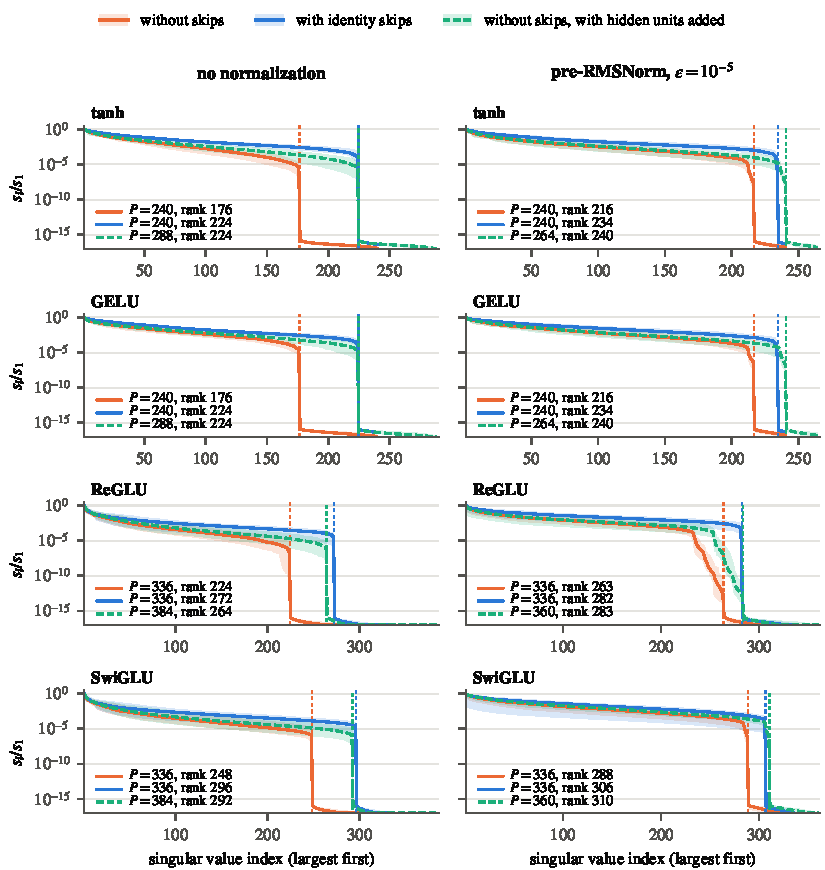
\includegraphics[width=\linewidth]{figs/spectra.pdf}
\caption{Singular values of the Jacobian on $4000$ inputs, for the networks of \cref{fig:gelu} with four kinds of blocks, and without skips with hidden units added; left without normalization, right with pre-RMSNorm. Dashed lines mark the rank. It equals the symmetry count in every draw, except for skipless ReGLU networks under RMSNorm.}
\label{fig:spectra}
\end{figure}

\para{The networks of \cref{fig:spectra}.} Every network of \cref{fig:spectra} is drawn $20$ times, and so are the same networks with GeGLU blocks and with GLU blocks, whose gate is the logistic sigmoid; both have the counts of SwiGLU. Except for the skipless ReGLU networks under RMSNorm, the rank equals the count in every draw, at gaps of at least $6\times10^{4}$ without normalization and $10^{7}$ under RMSNorm with $\varepsilon = 10^{-5}$. In the skipless ReGLU networks under RMSNorm, at gaps between $40$ and $2\times10^{4}$, the rank read at the largest gap is $263$ in $14$ draws, the count $264$ in $5$ and $253$ in one, and with hidden units added $283$ in $19$ draws and the count $284$ in one. With $\varepsilon = 10^{-12}$ the skipless ReGLU network has rank $233$ in every draw, at gaps of at least $10^4$: this is $P - L\dm^2 - (\dm(\dm-1)/2 + 1) - s$, the count of the network in which every normalization but the last is removed. The residual ReGLU network then has rank $281 = P - (\dm(\dm-1)/2 + 1) - s$ in every draw (\cref{sec:measured}). With $\varepsilon = 10^{-2}$ the rank equals the count in every draw for all six activations, ReGLU included, at gaps of at least $2.8\times10^{9}$; the notebook also plots these spectra as in \cref{fig:spectra}.

\para{The size of $\varepsilon$.} RMSNorm divides a row $h^{(t)}$ by $\sqrt{r^2 + \varepsilon}$, where $r^2 = \norm{h^{(t)}}^2/\dm$ is its mean square, so $\varepsilon$ acts relative to $r^2$. With inputs of unit variance, the median of $r^2$ over the inputs, and then over the draws, is $0.74$ at $h_0$ and between $0.15$ and $0.33$ after the blocks of the skipless networks, and it grows along the stream of the residual networks to between $1.6$ and $1.9$ at $h_3$; at these medians $\varepsilon/r^2$ lies between $5\times10^{-6}$ and $7\times10^{-5}$ for $\varepsilon = 10^{-5}$, and is about a thousand times larger for $\varepsilon = 10^{-2}$. In a skipless network every block reads a normalized state, so the scale of the inputs enters only at $h_0$; the stream of a residual network carries it to every hidden state. At $\varepsilon = 10^{-5}$ the singular values with indices $234$ to $264$ of the skipless ReGLU network, those of the $31$ directions of \cref{sec:measured}, lie between $10^{-4.5}$ and $10^{-12.6}$ of the largest in the median over the draws, except the last, which lies at the floor. The factors $\varepsilon/(r^2 + \varepsilon)$ that break these directions depend on the input, and they are large for the inputs whose hidden states have a small mean square: in every draw, between $11$ and $592$ of the $4000$ inputs have a hidden state after a block with $r^2 < 10^{-3}$, where $\varepsilon/r^2 > 10^{-2}$, and in $13$ of the $20$ draws up to $378$ inputs have one that is exactly zero, with every gate closed.

\para{Trained networks.} We also train the networks of \cref{fig:spectra}, with $\tanh$, GELU, ReGLU and SwiGLU blocks, on four classification datasets with at least four classes: two generated with scikit-learn, and satimage and segmentation from the Penn Machine Learning Benchmarks, with the features as inputs and one output per class. Training uses AdamW in single precision, a learning rate chosen on a validation set, early stopping and five seeds. A network counts as trained when it beats logistic regression with a tuned penalty on the test set, as $436$ of $480$ do. On inputs of the dataset and on Gaussian inputs alike, the rank equals the count in $398$ of the $436$, and the skips add $48$ and $18$ (\cref{fig:trained}). Of the $38$ exceptions, $36$ are skipless ReGLU networks under RMSNorm; one residual GELU network is $8$ below the count and one residual $\tanh$ network $1$ below. Two further notebooks train these networks, store them and compute their Jacobians.

\begin{figure}[t]
\centering
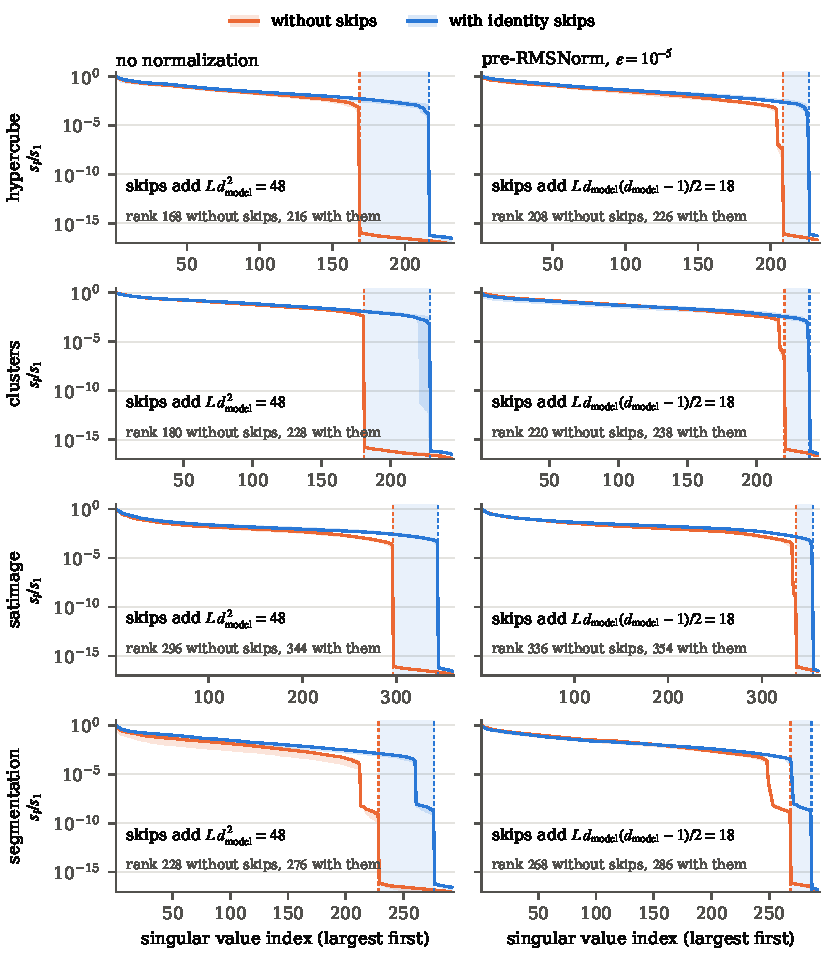
\includegraphics[width=\linewidth]{figs/spectra_trained_gelu.pdf}
\caption{Singular values of the Jacobian at trained weights, on $1000$ inputs of each dataset: the GELU networks of \cref{fig:spectra}, trained on four datasets (rows); median and range over five seeds. The skips add $L\dm^2$, and $L\dm(\dm-1)/2$ under RMSNorm, as at random weights.}
\label{fig:trained}
\end{figure}

\begin{table}[ht]
\centering\footnotesize\setlength{\tabcolsep}{2pt}
\caption{Functional-dimension checks. \emph{Rank} is the rank of the Jacobian on the batch; where the redundancy, $P$ minus it, equals the prediction, the rank meets the upper bound of \cpref{thm:count}{ii} and is the functional dimension. Every network has an embedding and a separate readout, and no biases unless marked; normalization is pre-norm. A \emph{mixed} skip is a pair of trainable identity units $U$, $V$ per block. The MLP networks have $\dm = 4$, width $8$, $L = 3$ unless marked, and input and output dimension $6$, except the rows marked \emph{large}, which have $\dm = 16$, $L = 6$, width $16$ and input and output dimension $20$. The transformers have $\dm = 8$, two heads of width four, MLP width $16$, a vocabulary of $16$ tokens and two layers; each attention block has $2Hd_h^2$ symmetries inside. $^\dagger$The exact rank modulo a prime certifies the value at two parameter points; without skips at $L = 3$, the rank in floating point sits at the double-precision floor. $^\ddagger$The symmetry count is $268$; an embedding table read through RMSNorm adds $\dm(\dm+1)/2 = 36$, because $N$ maps $\R^{\dm}$ onto an open ball, so the rows of the table can absorb any invertible map near the identity, and with continuous inputs the measured value is $268$.}
\label{tab:checks}
\begin{tabular}{@{}lllrrrl@{}}
\toprule
Network & Skip & Normalization & $P$ & Rank & Redundancy & Prediction \\
\midrule
$\tanh$ & none & none & 240 & 176 & 64 & $(L{+}1)\dm^2 = 64$ \\
$\tanh$ & identity & none & 240 & 224 & 16 & $\dm^2 = 16$ \\
$\tanh$ & learned & none & 288 & 224 & 64 & $(L{+}1)\dm^2 = 64$ \\
$\tanh$ & mixed & none & 336 & 224 & 112 & $(2L{+}1)\dm^2 = 112$ \\
$\tanh$, biases & none & none & 286 & 206 & 80 & $(L{+}1)(\dm^2{+}\dm) = 80$ \\
$\tanh$, biases & identity & none & 286 & 254 & 32 & $\dm^2 + (L{+}1)\dm = 32$ \\
\addlinespace
$\tanh$ & none & RMSNorm, $\varepsilon = 10^{-9}$ & 240 & 212 & 28 & $(L{+}1)\dim\CO(4) = 28$ \\
$\tanh$ & identity & RMSNorm, $\varepsilon = 10^{-9}$ & 240 & 233 & 7 & $\dim\CO(4) = 7$ \\
$\tanh$ & learned & RMSNorm, $\varepsilon = 10^{-9}$ & 288 & 260 & 28 & $(L{+}1)\dim\CO(4) = 28$ \\
$\tanh$ & none & RMSNorm, $\varepsilon = 10^{-2}$ & 240 & 216 & 24 & $(L{+}1)\dim\Ort(4) = 24$ \\
$\tanh$ & identity & RMSNorm, $\varepsilon = 10^{-2}$ & 240 & 234 & 6 & $\dim\Ort(4) = 6$ \\
$\tanh$ & learned & RMSNorm, $\varepsilon = 10^{-2}$ & 288 & 264 & 24 & $(L{+}1)\dim\Ort(4) = 24$ \\
\addlinespace
ReLU$^2$ & none & none & 240 & 152 & 88$^\dagger$ & $(L{+}1)\dm^2 + Lm = 88$ \\
ReLU$^2$ & identity & none & 240 & 200 & 40$^\dagger$ & $\dm^2 + Lm = 40$ \\
ReGLU & none & none & 336 & 224 & 112$^\dagger$ & $(L{+}1)\dm^2 + 2Lm = 112$ \\
ReGLU & identity & none & 336 & 272 & 64$^\dagger$ & $\dm^2 + 2Lm = 64$ \\
ReLU$^2$, $L = 8$ & none & none & 560 & 352 & 208$^\dagger$ & $(L{+}1)\dm^2 + Lm = 208$ \\
ReLU$^2$, $L = 8$ & identity & none & 560 & 480 & 80$^\dagger$ & $\dm^2 + Lm = 80$ \\
ReGLU, $L = 8$ & none & none & 816 & 544 & 272$^\dagger$ & $(L{+}1)\dm^2 + 2Lm = 272$ \\
ReGLU, $L = 8$ & identity & none & 816 & 672 & 144$^\dagger$ & $\dm^2 + 2Lm = 144$ \\
\addlinespace
$\tanh$, large & none & none & 3712 & 1920 & 1792 & $(L{+}1)\dm^2 = 1792$ \\
$\tanh$, large & identity & none & 3712 & 3456 & 256 & $\dm^2 = 256$ \\
$\tanh$, large & none & RMSNorm, $\varepsilon = 10^{-2}$ & 3712 & 2872 & 840 & $(L{+}1)\dim\Ort(16) = 840$ \\
$\tanh$, large & identity & RMSNorm, $\varepsilon = 10^{-2}$ & 3712 & 3592 & 120 & $\dim\Ort(16) = 120$ \\
\addlinespace
transformer & identity & RMSNorm, $\varepsilon = 10^{-2}$ & 1280 & 1124 & 156 & $\dim\Ort(8) + 4Hd_h^2 = 156$ \\
transformer & none & RMSNorm, $\varepsilon = 10^{-2}$ & 1280 & 976 & 304$^\ddagger$ & $5\dim\Ort(8) + 4Hd_h^2 = 268$ \\
\bottomrule
\end{tabular}
\end{table}

\para{Learned skips.} The $\tanh$ networks of \cref{tab:checks} with learned skips or with trainable identity units have the functional dimension of the residual network, $224$, as \cpref{thm:gaugefull}{ii} requires. Under RMSNorm with $\varepsilon = 10^{-2}$, learned skips have $264 - 234 = 30 = 3\,\dm(\dm+1)/2$ more functional dimension than identity skips, as \cpref{thm:rmsfull}{iii} predicts. On residual networks without biases or normalization ($\dm = 4$, $L = 3$, width $8$), spending the last change of basis on $\dm$ columns of the first read leaves exactly the redundancy $s$ of the symmetries inside the blocks, the last row of \cref{tab:ledger}.

\para{Low-rank skips.} Networks with skips $I + UV^\top$ ($L = 3$ $\tanh$ blocks of width $2\dm$, $\dm = 4$ with $r = 1, 2$ and $\dm = 6$ with $r = 2, 3$, exact Jacobians) have redundancy $\dm^2 + 2L\dm r$ without normalization, all of $U$ and $V$ besides the global change of basis, and $\dm(\dm-1)/2 + Lr(2r-1)$ under RMSNorm with $\varepsilon = 10^{-2}$. Besides the global rotation and the $r^2$ dimensions of the $\GL(r)$ inside each product, each skip adds $r(r-1)$. To first order, rotations $I + \Omega_{\ell-1}$ and $I + \Omega_\ell$ of the two hidden states that it joins change it by $(\Omega_\ell - \Omega_{\ell-1}) - \Omega_{\ell-1}UV^\top + UV^\top\Omega_\ell$, which keeps it within rank $r$ of the identity when $\Omega_\ell - \Omega_{\ell-1}$ lies in the tangent space $\{XV^\top + UY^\top\}$ of the matrices of rank $r$ at $UV^\top$; the antisymmetric matrices in this space have dimension $r(r-1)$ when $2r \le \dm$ and $U$, $V$ are generic, which the notebook confirms in every case.

\para{Where the redundancy exceeds the count.} For ReLU networks the exact Jacobian is taken with the activation pattern held fixed. On skipless ReLU networks without biases ($\dm = 4$, $L = 3$, width $8$), 7 of 8 random draws attain the bound of \cpref{thm:count}{ii}, redundancy $88$ including the rescalings of hidden units, and all 8 residual draws attain their bound, $40$. In the eighth skipless draw, five units of the last block are active on exactly the same inputs, those on which one unit of the block before is active, so there they act as one linear map of $\R^4$: their $40$ parameters carry $40 - 16 = 24$ dimensions of redundancy instead of the $5$ rescalings of the count, and the redundancy is $88 + 19 = 107$. Such coincidences need a block that reads the output of another block, so they do not occur for one block, where \cref{thm:onelayer} applies; this is consistent with \citet{grigsby2023hidden}. On the 3000 inputs of Section~1 of the notebook, a second draw also seems to exceed the bound, by 6, because one of its units is active on only $0.08$ percent of the inputs; with $30{,}000$ inputs or more it attains the bound, and the eighth draw stays at $107$ (Section~15 of the notebook). Skipless networks whose first hidden state is an embedding table read through RMSNorm are also more redundant than their symmetries (\cref{tab:checks}).

\para{Certificates at depth.} The rows of \cref{tab:checks} at $L = 8$ are certified as those at $L = 3$, with the activation pattern from ball arithmetic and the Jacobian from reverse mode (Section~16 of the notebook). Without skips these networks start from odd pairs of units, plus noise: ReLU$^2$ units $(u, w)$ and $(-u, -w)$, and ReGLU units with gates $u$ and $-u$ that share their value and write. With identity skips the weights are Gaussian, with the writes scaled by $1/L$. From Gaussian weights, the skipless ReGLU networks at $L = 8$ attain the count on $12{,}000$ inputs, and the ReLU$^2$ ones do not. In each ReLU$^2$ draw, $1$ to $5$ units of the last three blocks stay off on $2\times10^6$ fresh inputs, and a unit that is never on leaves its $8$ parameters redundant, $7$ more than its rescaling. With inputs added on which the rarely active units fire, the rank stays below the count by $35$, $7$ and $29$: $7$ for each unit that stays off, and one more in the third draw.

\para{DyT and nanoGPT.} DyT networks ($\dm = 4$, $L = 3$ blocks of width $8$, exact Jacobians, three draws) lose $L = 3$ dimensions to the skips, the scale of each hidden state, which the learnable $\alpha$ of the next DyT absorbs. The nanoGPT models of \cref{tab:nanogpt} follow the \texttt{model.py} of nanoGPT \citep{karpathy2023nanogpt}, with token and position embeddings, pre-LayerNorm blocks with $\varepsilon = 10^{-5}$, causal attention with four heads of width two, GELU MLPs of width $4\dm$, a final LayerNorm and a readout, and no biases; without normalization every LayerNorm is the identity. The Jacobians are exact, over all logits of $64$ random token sequences per layer. With skips the redundancy is, per layer, $144$ with LayerNorm: $32$ from the changes of basis inside the heads, $16$ from the LayerNorm gains against the next matrix, $56$ from the zero mean of each LayerNorm output, seen by every column of the next matrix, and $40$ from the mean of each write, which every later LayerNorm erases. Once per model come $60$ more: the global rotation, $21$; the means of the $16$ embedding rows, $16$; the final LayerNorm against the readout, $16$; and a vector moved from the position to the token embedding, $7$. Without normalization it is $32$ per layer and $72 = 64 + 8$ per model. For one and two layers we construct all of these symmetries, and in every draw they span the null space of the Jacobian.

\begin{table}[ht]
\centering\small
\caption{Redundancy of nanoGPT ($\dm = 8$, four heads of width two, a vocabulary and a context of $8$, no biases, untied readout): $P$ minus the rank of the exact Jacobian, the same in all four draws of every network and equal to the prediction. $N$ layers make $L = 2N$ blocks. With skips, each layer is redundant by $144$ with LayerNorm and by $32$ without normalization, and the model once more by $60$ and $72$ (\cref{app:checks}).}
\label{tab:nanogpt}
\begin{tabular}{lrrrrl}
\toprule
& $N = 1$ & $2$ & $3$ & $4$ & Prediction \\
\midrule
\multicolumn{6}{@{}l}{\emph{LayerNorm}} \\
$P$ & 984 & 1768 & 2552 & 3336 & \\
without skips & 246 & 432 & 618 & 804 & $144N + 60 + 21L$ \\
with skips & 204 & 348 & 492 & 636 & $144N + 60$ \\
\addlinespace
\multicolumn{6}{@{}l}{\emph{No normalization}} \\
$P$ & 960 & 1728 & 2496 & 3264 & \\
without skips & 232 & 392 & 552 & 712 & $32N + 72 + 64L$ \\
with skips & 104 & 136 & 168 & 200 & $32N + 72$ \\
\bottomrule
\end{tabular}
\end{table}

\para{Notebook.} The notebook runs on a CPU in an environment pinned with uv, with Python~3.11. Its sections follow the paper and are listed below, with their times on a CPU with two cores. The two long experiments save what \cref{fig:spectra} and \cref{tab:nanogpt} need, from which the notebook draws the figure and the table in seconds unless it is asked to rerun them; the times below are those of the full computation.

\begin{center}\small
\begin{tabular}{@{}p{0.4\textwidth}p{0.43\textwidth}l@{}}
\toprule
Section of the notebook & What it reproduces & Time \\
\midrule
1. The gauge fix, the counts and RMSNorm & exactness checks of \cref{thm:gaugefull,thm:rmsfull,prop:normalform}; finite-difference rows of \cref{tab:checks}; exact ReLU and degree-two Jacobians & 1 min \\
2. The last row of \cref{tab:ledger} & the last row of \cref{tab:ledger} & 23 s \\
3. A dominant block, and learned, tied and low-rank skips & the checks of \cref{sec:gaugefix,sec:norm,sec:reduce} & under 1 s \\
4. The redundancy of low-rank skips & the low-rank skips of \cref{sec:norm} & 36 s \\
5. DyT reads & the DyT networks & 9 s \\
6. Exact reductions after training & the reductions of \cref{sec:skipless} and \cref{prop:ln} & under 1 s \\
7. The symmetry group of a transformer is not a product & \cref{tab:product} & under 1 s \\
8. Counts at model scale & \cref{tab:scale} & under 1 s \\
9. One block & \cref{thm:onelayer}, for MLP and attention blocks & 44 s \\
10. \Cref{fig:spectra} & \cref{fig:spectra,fig:gelu} and the checks of their networks & 28 min \\
11. Exact Jacobians & the rows at $\dm = 16$, the transformers and the embedding table of \cref{tab:checks} & 4 min \\
12. Certificates modulo a prime & the certificates at $L = 3$ in \cref{tab:checks} & 19 s \\
13. nanoGPT & \cref{tab:nanogpt} and the constructed symmetries & 38 min \\
14. Skipless networks as limits of residual networks & the limits of the companion paper & under 1 s \\
15. ReLU draws above the count & the ReLU draws above the count in \cref{app:checks} & 2 min \\
16. Certificates at depth & the certificates at $L = 8$ in \cref{tab:checks} & 5 min \\
17. Homogeneous blocks under RMSNorm & the checks of \cref{lem:homrms} & 2 s \\
\bottomrule
\end{tabular}
\end{center}

\end{document}
